%%%%%%%%%%%%%%%%%%%%%%%%%%%%%%%%%%%%%%%%%%%%%%%%%%%%%%%%%%%%%%%%%%%%%%%%%%%%%%%%%%%%%%%%%%%%%%%%%%%%%
%
%   Version     : 2.0
%
%   Filename    : main.tex
%
%   Description : This is the main file for the LaTeX thesis proposal document template.
%                 The template is intended for use by BSCS students. 
%
%                It is assumed that you can learn how to use LaTeX on your own.
%                Please check/read the following online LaTeX book:
%
%                                 http://en.wikibooks.org/wiki/LaTeX
%     
%   Author      : Florante R. Salvador
%
%   Contributors: 1.  Karlo Campos 
%                     a. margin settings for DLSU thesis paper 
%   
%   Notes       : Please email florante.salvador@dlsu.edu.ph for comments, suggestions, ideas etc.
%
%   Reference:
%
%
%   History/Updates:
%      March 12, 2009 -- created version 1.0 for release to CSC701M (Methods of Research) students
%      May 30, 2009   -- updated Title page and Abstract for undergrad ST students
%
%      Feb 27, 2015 -- Created Version 2 (major overhaul): changed class to report, created a figures folder, 
%                               removed unnecessary packages, added new comments  based on Ethel Ong's slides
%
%%%%%%%%%%%%%%%%%%%%%%%%%%%%%%%%%%%%%%%%%%%%%%%%%%%%%%%%%%%%%%%%%%%%%%%%%%%%%%%%%%%%%%%%%%%%%%%%%%%%%%


%%%%%%%%%%%%%%%%%%%%%%%%%%%%%%%%%%%%%%%%%%%%%%%%%%%%%%%%%%%%%%%%%%%%%%%%%%%%%%%%%%%%%%%%%%%%%%%%%%%%%%%%%%%%%%%%%%%%%%%
%
%  Filename   : preamble.tex
%
%  Description: Preamble file to :
%               a. specify related packages
%               b. set margins, commands, etc.
%
%  Note       : Edit the margin settings for your own printer
%                  You may add your own commands, environments (it is assumed that you know what you're doing.)
%
%%%%%%%%%%%%%%%%%%%%%%%%%%%%%%%%%%%%%%%%%%%%%%%%%%%%%%%%%%%%%%%%%%%%%%%%%%%%%%%%%%%%%%%%%%%%%%%%%%%%%%%%%%%%%%%%%%%%%%%

%\documentclass[12pt,titlepage,onepage, letterpaper]{article}

\documentclass[12pt,titlepage,onepage, letterpaper]{report}

\setcounter{secnumdepth}{4}
\setcounter{tocdepth}{4}

\usepackage{xr}\externaldocument{chapter_4}
\usepackage{longtable}
\usepackage{enumitem}
\usepackage{multicol}
\usepackage[normalem]{ulem}

%
%-- specify related packages
%

%
% \usepackage[utf8x]{inputenc}
%

\usepackage{apacite}           %-- APA style citation 
                               %-- refer to http://www.ctan.org/tex-archive/biblio/bibtex/contrib/apacite/

%
%  \usepackage{ucs}
%


\usepackage{amsmath}           %-- American Math Society packages
\usepackage{amsfonts}
\usepackage{amssymb}


\usepackage{graphicx}          %-- graphicx package needed for including figures in JPG or PNG format

\usepackage{pdfpages}	%-- include PDF Documents
 
%
%\usepackage{graphics}          %-- graphics related package (this was commented out) use when image is in EPS format
%

\usepackage{verbatim}          %-- this package allows you to have multiple lines of comments by
                               %-- example:
                               %   \begin{comment}
                               %        ...your text here...
                               %   \end{comment}  

\usepackage{color}             %-- allows use of color with text
                               %-- example:  \textcolor{red}{This is the colored text in red.}

\usepackage{url}  %-- allows use of URLs example: \url{https:\ccs1.dlsu.edu.ph}


%
%-- set margins,  you may need to edit this for your own printer
%
\topmargin 0.0in
\oddsidemargin 0.0in
\evensidemargin 0.0in

\voffset 0.0in
\hoffset 0.5625in

\textwidth 5.75in
\textheight 8.5in


\parskip 1em
\parindent 0.25in


\bibliographystyle{apacite}            %-- use APA citation scheme

\hyphenation{ana-lysis know-ledge}     %-- LaTeX may not hyphenate correctly some words you use in your document
                                       %-- use \hyphenation to instruct LaTeX how to do it correctly, example above

\newcommand{\degree}{^{\circ}}         %-- use \newcommand to create your own "commands"
                                       %-- \newcommand works like the #define you learned in your COMPRO1 class

\newcommand{\etal}{et al.}


%\newcommand{\sinag}{\emph{Sinag}}
%\newcommand{\sinagtwo}{\emph{Sinag2}}

\newcommand{\figref}[1]{Figure \ref{#1}}
\newcommand{\appref}[1]{Appendix \ref{#1}}

%-- \newcommand{\Section}[1]{\section{#1}\setcounter{figure}{0}\setcounter{table}{0}}

%\newcommand{\shade}{\multicolumn{1}{|>{\columncolor[gray]{0.25}}c|}{}}
%\newcommand{\tableheader}[1]{\rowcolor{black}\color{white}{#1}}
%\newcommand{\cell}[2]{\multicolumn{1}{#1}{#2}}
%\newcommand{\definition}[2]{\textbf{\textit{#1}} --- #2}
%\newcommand{\itembit}[1]{\item \textbf{\textit{#1}}}
%\newcommand{\sgdef}[2]{\parbox[t][][t]{1.75in}{\textbf{#1}} \> \parbox[t][][t]{4.0in}{#2}\\\\}

%\newenvironment{sinagglossary}{\begin{flushleft}
%\begin{tabbing}
%\hspace{1.75in}\=\\}{\end{tabbing}\end{flushleft}}

\newcommand{\thestitle}[1]{{\Large \textsc{#1}}}

%---
%  \renewcommand{\thefigure}{\thesection.\arabic{figure}}
%  \renewcommand{\thetable}{\thesection.\arabic{table}}
%  \renewcommand{\contentsname}{Table of Contents}




                %-- includes LaTeX source file for the preamble 
                                  %-- include packages, sets the margin sequence, and many more... 
                                  %-- your job: check if the settings are suitable for your own printer

\graphicspath{{figures/}}  %-- figures is the name of the folder containing images JPG or PN

\usepackage{rotating}
\usepackage{float}
\usepackage{longtable}

\begin{document}

%%%%%%%%%%%%%%%%%%%%%%%%%%%%%%%%%%%%%%%%%%%%%%%%%%%%%%%%%%%%%%%%%%%%%%%%%%%%%%%%%%%%%%%%%%%%%%%%%%%%%%
%
%   Filename    : title_page.tex 
%
%   Description : This file will contain your Title Page.
%                 
%%%%%%%%%%%%%%%%%%%%%%%%%%%%%%%%%%%%%%%%%%%%%%%%%%%%%%%%%%%%%%%%%%%%%%%%%%%%%%%%%%%%%%%%%%%%%%%%%%%%%%

\begin{titlepage}
\centering


%-- **EDIT** the following line to indicate your thesis title
\thestitle{Generating Life Stories From Facebook Posts}

\vspace{1.75cm}
A Thesis\\
Presented to\\
the Faculty of the College of Computer Studies\\
De La Salle University-Manila

\vspace{1.75cm}
In Partial Fulfillment\\
of the Requirements for the Degree of\\
Bachelor of  Science in Computer Science

\vspace{1.75cm}
by\\
%-- **EDIT** the following line to indicate your name 
\vspace{1cm}

HADE, Alden Luc R. \\
LAM, Janica Mae M.  \\
SAAVEDRA, Camille Alexis T.R.  \\
TE, Robee Khyra Mae J. \\

\vspace{1.75cm}
%-- **EDIT** the following line to indicate your adviser's name 
Ethel Chua Joy ONG \\
Adviser

\vspace{1.75cm}
July 13, 2017 \\ %-- \today
\end{titlepage}
              %-- includes LaTeX source file for the Title Page 
                                  %-- your job: **EDIT THIS FILE ** to indicate your own title, name, and thesis adviser's name


%%%%%%%%%%%%%%%%%%%%%%%%%%%%%%%%%%%%%%%%%%%%%%%%%%%%%%%%%%%%%%%%%%%%%%%%%%%%%%%%%%%%%%%%%%%%%%%%%%%%%%
%
%   Filename    : abstract.tex 
%
%   Description : This file will contain your abstract.
%                 
%%%%%%%%%%%%%%%%%%%%%%%%%%%%%%%%%%%%%%%%%%%%%%%%%%%%%%%%%%%%%%%%%%%%%%%%%%%%%%%%%%%%%%%%%%%%%%%%%%%%%%

\begin{abstract}
People love sharing stories with one another because stories provide them with enjoyable experiences as well as help them learn new things. Nowadays, people use social media, and in particular, Facebook, to share information about themselves, their daily activities and the things that interest them. However, a Facebook user’s data (posts, photos, personal info, etc.) by itself does not provide a \textit{concise} narrative of events that can be used to adequately tell a person’s life story. 

There is no current work implemented which creates a textual story from a given set of user-generated social media data. This research focuses on automatically generating a life story from a person's Facebook text posts. To this end, a system called FB Stories was developed. It extracts user data from Facebook (with their permission), processes them, organizes them into different types according to their text content, and utilizes this knowledge in order to generate a person’s life story. 

The development of the system showed the difficulty of working with noisy user-generated data. The testing showed that, while there were issues with low precision and high recall, the system addresses the research gap and satisfies all of its objectives. 

\begin{flushleft}
\begin{tabular}{lp{4.25in}}
\hspace{-0.5em}\textbf{Keywords:}\hspace{0.25em} &Social media, Facebook, Text understanding, Post classification, Life event detection, Storytelling, Story generation \\
\end{tabular}
\end{flushleft}
\end{abstract}
                %-- this is the Abstract page
                                  %-- your job: **EDIT THIS FILE** to indicate your own abstract


\pagenumbering{roman}             %-- this will number pages as i, ii, iii, etc...
\setcounter{page}{2}

\tableofcontents                  %-- this command is used to generate the Table of Contents


\newpage
\listoffigures                    %-- this command is used to generate List of Figures

\newpage                       
\listoftables                     %-- this command is used to generate List of Tables


\newpage

\pagenumbering{arabic}            %-- this will number pages as 1, 2, 3, etc...
\setcounter{page}{1}              


%%%%%%%%%%%%%%%%%%%%%%%%%%%%%%%%%%%%%%%%%%%%%%%%%%%%%%%%%%%%%%%%%%%%%%%%%%%%%%%%%%%%%%%%%%%%%%%%%%%%%%
%
%   Filename    : chapter_1.tex 
%
%   Description : This file will contain your Research Description.
%                 
%%%%%%%%%%%%%%%%%%%%%%%%%%%%%%%%%%%%%%%%%%%%%%%%%%%%%%%%%%%%%%%%%%%%%%%%%%%%%%%%%%%%%%%%%%%%%%%%%%%%%%

\chapter{Research Description}
\label{sec:researchdesc} 

This chapter explains the concept of stories as an important part of human life. It introduces the current state of technology, and discusses the objectives of the research, the scope and limitations, and the significance of the study.

%section~~~~~~~~~~~~~~~~~~~~~~~~~~~~~~~~~~~~~~~~~~~~~~~~~~~~~~~~~~~~~~
\section{Overview of the Current State of Technology}
\label{sec:overview}

The world is full of stories. In his book, \textit{The Storytelling Animal}, Jonathan Gottschall says that human beings are natural storytellers -- ``that they can't help telling and \textit{creating} stories because they like narratives so much" \cite{Gopnik2012}.

Storytelling is an ancient and abiding art. It is one of the things that distinguishes human beings from animals. The reasons why people love stories vary from person to person -- \textit{history} shows that for the longest time, humans loved to tell stories \cite{Gopnik2012}; \textit{theologians} tell stories because their moral lessons influence readers to become better people; and \textit{biology} claims that compared to when one simply explains things to someone, telling a story puts their whole brain to work \cite{Widrich2012} -- but in summary, people love sharing stories because they provide them with enjoyable experiences as well as help them learn. Stories also serve as a reflection of people's own experiences, and they are an effective route in reaching out and connecting to others.

The world of storytelling has changed over the course of history, from oral tradition to online technology. Nowadays, computers are still not capable of fully developing and telling stories on their own; recently however, more storytelling systems (also known as \textit{story generation systems}) are being developed as part of artificial intelligence (AI) trends to build solutions that could support and mimic human tasks.

Aside from storytelling systems, the digital age introduced society to the concept of social media, another method through which people's stories could be preserved. The introduction of social media has allowed storytelling to become more immersive, as it has employed a combination of text, photo, and video in a way that has become more participatory. 

A \textit{social networking site (SNS)} or social media is defined as ``a web-based system that allows individuals to (1) construct a public or semi-public profile within a bounded system, (2) articulate a list of other users with whom they share a connection, and (3) view and traverse their list of connections and those made by others within the system" \cite{BoydEllison2010}. The most popular SNS at the time of this writing is Facebook, which allows users to create their own profile with information about themselves; observe other users' content; and interact with others through reacting, commenting, and sharing. By far the biggest social network worldwide, Facebook has an estimate of over 1.71 billion monthly active users, as of 2016 \cite{Harden2016}.

Facebook is emerging as a near-universal storytelling method. One of the things that make Facebook successful is the unique, freeform nature in which it allows users to share information. Facebook's \textit{timeline} feature provides people with their own way of creating a complete story about themselves, from their birth to the current day. Users, pages, groups, and events each have a timeline containing posts that they are involved in. Information on Facebook can consist of many forms: from text, to photo, to video. These small acts of posting and updating one's status about current events and occurrences on Facebook can be considered small stories as the posts are arranged chronologically similar to a storyline \cite{West20131}. 

Recognizing the appeal and importance of remembering past events, Facebook has recently implemented a feature called \textit{On This Day}, which notifies users of posts that happened on a particular day in the past several years. Facebook also has a feature called \textit{Year in Review}, which collects photos from what Facebook determines to be the user's most significant moments in the past year. However, while Facebook already has features that can potentially tell stories about a person's life through pictures, there is no current work implemented which creates a textual story of a user's Facebook account. Research works in automated story generation have also not explored the use of user-created content (such as social media posts) as a source of knowledge for planning the content of a story to be generated.

%section~~~~~~~~~~~~~~~~~~~~~~~~~~~~~~~~~~~~~~~~~~~~~~~~~~~~~~~~~~~~~~
\section{Research Objectives}
\label{sec:researchobjectives}

This section presents the general and specific objectives of the research in order to be able to address this research gap.

\subsection{General Objective}
\label{sec:generalobjective}

To develop an application that generates one's story using data collected from his/her Facebook account.

\subsection{Specific Objectives}
\label{sec:specificobjectives}

\begin{enumerate}
   \item To define a life story and determine its elements and structure;
   \item To review the content of Facebook and the existing methods used in extracting data from Facebook;
   \item To design an algorithm for understanding user-created text content;
   \item To build a knowledge base from which to model the story structure and to supplement the data extracted from Facebook;
   \item To select which post types and post classification algorithm to use in classifying each Facebook post;
   \item To analyze story generation algorithms and design an algorithm for generating stories using data from Facebook; and
   \item To define the metrics to be used in evaluating the generated story.
\end{enumerate}

%section~~~~~~~~~~~~~~~~~~~~~~~~~~~~~~~~~~~~~~~~~~~~~~~~~~~~~~~~~~~~~~
\section{Scope and Limitations of the Research}
\label{sec:scopelimitations}

A \textit{life story}, or a biography, is an account of the series of events making up a person's life according to The Free Dictionary \footnote{The Free Dictionary. http://www.thefreedictionary.com/}. In order to apply this concept in the research, the different elements which make up a life story should be examined. However, the idea of a story is not to capture every single detail, but to give the participants something to remember. Therefore, the more important and relevant elements that make up a good story should be determined.

A Facebook user's account can contain gigabytes of unnecessary data, which are irrelevant in generating a complete story. Therefore, this research needs to determine which types of content are appropriate for generating life stories. Furthermore, knowledge of the different types of methods of extracting data from Facebook allows the research to extract the data needed in generating a story.

The story will be based on user-generated data; therefore, consent is necessary not only to provide the necessary data but also to avoid violating privacy and confidentiality. The system to generate stories from Facebook posts will be launched by the users themselves, and not by somebody else. Graphic files such as images and videos will not be included in this research. The number of Likes for each post will be extracted but not the information about the actual users. Private messages will also not be included. Only posts composed in the English language will be used.

Story generation systems require certain predefined knowledge in order to do their task of generating stories. A knowledge base, which is defined as ``the underlying set of facts, assumptions, and rules which a computer needs to solve a problem" according to Oxford Dictionary \footnote{Oxford Dictionary. https://en.oxforddictionaries.com}, helps the system generate the story. This research requires identifying possible knowledge sources as well as designing an appropriate knowledge base structure to provide data to be used for generating a life story.

Social networking sites have been a crowd-sourced knowledge base of people's activities as well as real time events \cite{Jain2016TowardsAE}. Starbird and Palen (2011) stated that rescue workers use SNSs to know and talk to natural disaster survivors. In this research, for stories to have a better flow, it is important to classify posts accurately according to their types. However, there are many post types present in SNSs, and accommodating all these will not be possible in this research. Thus, only the most used post types will be selected. Different classification algorithms will also be reviewed to determine which ones can be adapted for this research.

Story generation algorithms (SGAs) will be reviewed in order to determine which ones are appropriate and can be adapted for the context of this research. These are computational procedures which result in an artifact that can be considered a story \cite{Gervas2012}. The concept of a story in SGAs is functional and not aesthetic, which means that having appealing text is not their primary concern. 

Finally, in order to measure the quality of the generated stories, a set of evaluation metrics will be defined. These metrics will then be used to evaluate the strengths and weaknesses of the system.

%section~~~~~~~~~~~~~~~~~~~~~~~~~~~~~~~~~~~~~~~~~~~~~~~~~~~~~~~~~~~~~~
\section{Significance of the Research}
\label{sec:significance}

As mentioned in Section 1.1, despite the appeal of storytelling as part of human experience, computers are still not capable of fully developing and telling stories on their own, nor understanding stories being told by humans. This research, therefore, contributes to the field of computing technology by contributing to the field of story generation: by enabling computers to make sense of a wide variety of user-generated data in order to tell stories.

This research can be a first step needed by a smart computer to understand a person's life. With this, software agents can use information from Facebook data to make sense of a person's activities and experiences. This can help inform relevant stakeholders regarding aspects of lives of their constituents, with applications in social behavior analysis, community healthcare monitoring, and personalized digital marketing. 

This can lead to a better understanding of people, both as individuals and as a whole community, and open up possibilities of customization and personalization in computer-based support systems and interaction. Furthermore, this research can be of interest to writers and computer scientists looking to learn more about the fields of artificial intelligence and/or story generation.

%section~~~~~~~~~~~~~~~~~~~~~~~~~~~~~~~~~~~~~~~~~~~~~~~~~~~~~~~~~~~~~~
\section{Research Methodology}
\label{sec:methodology}
This section lists down and elaborates on the specific activities that will be performed by the proponents in the course of conducting the research. The discussion covers the activities from the start to the end of the research, including ethical issues.

\subsection{Research Activities}

\subsubsection{Review of Related Literature}
During this phase, existing works related to event classification, story generation systems, and text understanding are reviewed and analyzed. In addition, Facebook and other relevant social networking sites are examined to determine which ones are a relevant source for data to be used for the generation of a person's life story. A survey of data extraction tools will help the proponents identify the specific data that can be extracted from Facebook.

\subsubsection{Review of Ethical Issues}
In this phase, the ethical issues concerned with research are reviewed and identified. The General Research Ethics Checklist (Appendix \ref{sec:appendixe}) was accomplished to be able to identify potential risks to participants. This research involves Facebook users, thus, the Research Ethics Checklist for Investigations Involving Human Participants (Appendix \ref{sec:appendixf}) was also accomplished. 

The data collection process, the sources of data, the sampling details, and the data retention details were provided. Two Informed Consent Forms (Appendix \ref{sec:appendixg} and Appendix \ref{sec:appendixh}) were created to be filled up by the Facebook user and were used during the data gathering process and the actual testing of the software.

Aside from accomplishing these forms, specific steps to address ethical concerns have also been identified. The steps are discussed in Section 1.5.1.6 Testing and Evaluation of this document.

\subsubsection{Data Gathering and Analysis}
For this phase, sample life stories have been generated manually from the researcher's Facebook accounts to identify the elements present in a life story, and to have a better understanding of what sort of stories can mostly be generated from samples of data returned by Facebook's Graph API (described in Section 2.1, Data Extraction Tools).

Furthermore, to focus on identifying and analyzing the different elements that comprise a story, such as character, setting, and events, Facebook data from different users will be gathered. Part of the data analysis was also learning how the elements can fit each other and whether they are necessary or not in coming up with the story. From there, the scope was narrowed down to the elements that were deemed necessary, such as the subject's childhood, education, likes, and recent events in their life. The expertise of linguists and/or story writers have been consulted as necessary, as well as the knowledge gained from the Review of Related Literature.

\subsubsection{Software Design}
During this phase, the different modules of the story generation system have been designed. The different elements were identified as follows: (1) the user interface, (2) the knowledge base, (3) the algorithm for text understanding, (4) the algorithm for post classification, and (5) the algorithm for story generation.

The user interface (UI) will have to provide a convenient user experience; therefore, mockups and/or prototypes were created to assess the usability and effectiveness of the UI. Also, with the help of the sample stories gathered in 1.5.1.2, mock stories have been generated manually to get a better understanding of what sort of stories can mostly be generated from Facebook data. From these, story templates were created for generating the introduction part of the actual life stories. These templates were stored in a database with the data extracted from Facebook. Different approaches for post classification, text understanding, and story generation have also been studied in order to adapt an efficient algorithm to be used in the software. 

\subsubsection{Software Implementation}
The software will be implemented based on the design in 1.5.1.4 using the chosen language. Implementation and testing will be iterative processes to allow redesigning of the software and improvement of the algorithms to achieve the target objectives and produce better stories. Essential steps to follow in software implementation are (1) building the knowledge base, (2) implementing the algorithms for data extraction, post classification, text understanding, and story generation, and basically following the design specifications stated in Chapter 4.

The software development life cycle followed was Scrum, an iterative and incremental agile methodology which splits the whole process into smaller tasks. This development process has series of iterations called Sprints which lasts for no more than a month. This allowed easier adaptation to changes after performing unit testing to allow improvements on the current design.

\subsubsection{Testing and Evaluation}
The software was tested by several evaluators, who are Facebook users, linguists and story writers. Before the evaluation process, the following steps were conducted:

First, the metrics to be used by these evaluators were defined based on the evaluation metrics in Section 3.7 of this document.

Second, the software underwent usability testing to determine the ease of with which the user can interact with the interface to perform his/her tasks. This was an iterative process because testing and refining the software needs to be done repeatedly in order to ensure that the evaluation metrics are satisfactorily met. During the implementation (1.5.1.5) phase, the software being developed was periodically tested to validate its usability and correctness. Different test cases were designed and executed, such as checking the generated stories of various Facebook accounts. Implementation was continued in order to fix issues that arise.

Third, the Facebook users were briefed on the evaluation process by informing them of the following: (1) introduction of the research topic, (2) demonstration of how the software works, (3) signing of the informed consent, (4) confidentiality in storing the generated story from their Facebook accounts for further improvements, and (5) interview with the Facebook users for their experience in using the software as well as their feedback on the resulting stories. After this, the actual testing of the software was conducted in a room where a computer will be used for testing. Each session with a user lasted only for the duration of generating a minimum of one (1) story from the user's Facebook posts. The testing process ends after evaluating the generated story.

Fourth, an interview will be conducted after testing the software. The Facebook user was asked to answer a survey form containing metrics to evaluate the correctness and completeness of the generated story. Qualitative feedback was also solicited, including suggestions and recommendations to further improve the story generation.

Lastly, linguists and story writers were asked to evaluate the resulting stories using an evaluation form that is based on the evaluation metrics stated in Section 3.7 Evaluation Metrics of this document. These experts evaluated the quality of the generated story in terms of completeness and correctness. Suggestions and recommendations were also solicited to further improve the generated output.

Results from the testing process were used to determine the appropriateness and sufficiency of the knowledge sources and various data extracted from Facebook posts and their impact on the quality of the resulting stories.

\subsubsection{Documentation}
Documentation was done all throughout the duration of the research. The findings of each activity were documented accordingly.

\subsection{Calendar of Activities}

Table \ref{tab:timetableactivities} shows a Gantt chart of the activities. Each bullet represents approximately one week's worth of activity.

%
%  the following commands will be used for filling up the bullets in the Gantt chart
%
\newcommand{\weekone}{\textbullet}
\newcommand{\weektwo}{\textbullet \textbullet}
\newcommand{\weekthree}{\textbullet \textbullet \textbullet}
\newcommand{\weekfour}{\textbullet \textbullet \textbullet \textbullet}

\begin{sidewaystable}[ph!]   %t means place on top, replace with b if you want to place at the bottom
\centering
\caption{Timetable of Activities} \vspace{0.25em}
\begin{tabular}  {|p{2.1in}|c|c|c|c|c|c|c|c|c|c|c|c|c|c|c|}  \hline
   & \multicolumn{7}{c|}{2016} & \multicolumn{8}{c|}{2017}\\ \hline
\centering Activities & Jun & Jul & Aug & Sep & Oct & Nov & Dec & Jan & Feb & Mar & Apr & May & Jun & Jul & Aug\\ \hline
Review of Related Literature & \weekfour & \weekfour & \weekfour & ~\weekthree & \weekfour & \weekfour & & & & & & & & & \\ \hline
Data Gathering and Analysis & & & & ~\weekthree & \weekfour & \weekfour & \weektwo ~~ & & & & & & & & \\ \hline
Review of Ethical Issues & & & ~~\weektwo & & ~~\weektwo & & & & & & & & & & \\ \hline
System Design & & & & & \weekfour & \weekfour & \weektwo~~ & ~\weekthree & & & & & & & \\ \hline
System Implementation & & & & & & & & ~\weekthree & \weekfour & \weekfour & \weekfour & \weekfour & \weekfour & \weekfour & \weekone~~~  \\ \hline
Testing and Evaluation & & & & & & & & & & & ~~\weektwo & ~~\weektwo & ~~\weektwo & \weekfour & \weekone~~~  \\ \hline
Documentation & \weekfour  & \weekfour & \weekfour & ~\weekthree & \weekfour & \weekfour & \weektwo ~~ & ~\weekthree & \weekfour & \weekfour & \weekfour & \weekfour & \weekfour & \weekfour & \weekone~~~ \\ \hline
\end{tabular}
\label{tab:timetableactivities}
\end{sidewaystable} 

%%%%%%%%%%%%%%%%%%%%%%%%%%%%%%%%%%%%%%%%%%%%%%%%%%%%%%%%%%%%%%%%%%%%%%%%%%%%%%%%%%%%%%%%%%%%%%%%%%%%%%
%
%   Filename    : chapter_2.tex 
%
%   Description : This file will contain your Review of Related Literature.
%                 
%%%%%%%%%%%%%%%%%%%%%%%%%%%%%%%%%%%%%%%%%%%%%%%%%%%%%%%%%%%%%%%%%%%%%%%%%%%%%%%%%%%%%%%%%%%%%%%%%%%%%%


\chapter{Review of Related Literature}
\label{sec:relatedlit}

This chapter discusses the features, capabilities, and limitations of existing research, as well as the algorithms and/or software that are relevant to the study. 

%section~~~~~~~~~~~~~~~~~~~~~~~~~~~~~~~~~~~~~~~~~~~~~~~~~~~~~~~~~~~~~~
\section{Data Extraction Tools}
Data extraction is the process of crawling through data sources, such as a database, in order to retrieve information that can be used for further data processing or data storage \cite{Technopedia2016}. For this study, data extraction involves selecting needed data from Facebook as an input to the story generation system. 

Three data extraction tools that are relevant to the current study have been reviewed:
\begin{enumerate}
\item Download Facebook Data \cite{FacebookDownload, FacebookDownload2}
\item Graph API \cite{WeaverTarjan2013, FacebookGraphAndroid2016}
\item Facepager \cite{Facepager2016}
\end{enumerate}

Table \ref{tab:DataExtractionTool} shows a comparison of these data extraction tools.

\subsection{Download Facebook Data}
The simple act of logging in to Facebook is already a way of accessing data stored in Facebook. The Activity Log is a built-in Facebook feature that shows the history of activities done on Facebook. It includes likes, comments, search history, and others. In 2010, Facebook introduced a new feature where these data can be downloaded for the user's own purposes. This is a compilation of the user's own data on Facebook, such as the user's personal info, friends list, and messages, among others.

Facebook automatically compiles the data to be downloaded once the user chooses to archive his/her files. An email containing the download link would then be forwarded to the mail address registered in the user's account. Once downloaded, the .zip file includes all media posted by the user in Facebook. It also contains a file, index.html, which is an HTML file that acts similarly to Facebook's home page. It displays the user's profile data such as the Facebook link, email address, registration date, birthday, past Facebook names (if any), current city and hometown, and other information that the user has provided on this Facebook account. There are also several HTML files provided in the HTML folder for easier indexing and browsing, as shown in \figref{fig:fbdatazip}.

\begin{figure}[!htb]                %-- use [t] to place figure at top, [b] to place at the bottom, [h] for here
   \centering                    %-- use this to center the figure
   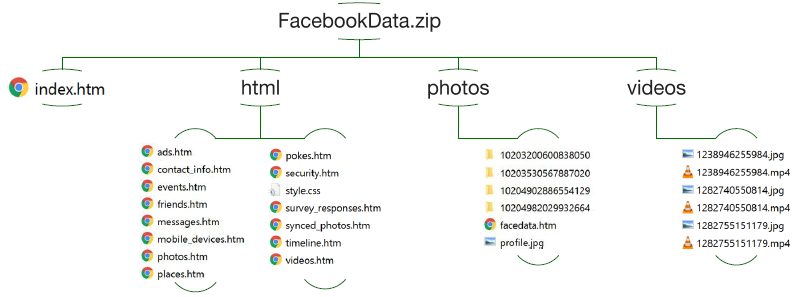
\includegraphics [width=\textwidth] {fbdatazip.png}      %-- include image file named as "disneychart.png" 
   \caption{Content of Facebook Data .zip File}
    \label{fig:fbdatazip}
\end{figure}

The date, time, timezone, tags, and source of posts that are shared are provided in the Timeline tab. Meanwhile, image and video files are separated from the description that comes along with it. Similar to the Timeline tab, the photos and videos tab also contains the time, date, and timezone of the media file posted. Aside from displaying the media file and the missing message of the post, the photos include the following details - the camera model, orientation, width, exposure, ISO speed, IP address and comments - while the videos include the thumbnail image and comments in the video.

\subsection{Graph API}
Facebook has developed the Graph API to allow developers to extract posts and other data from a specific Facebook page or a user's Facebook account. The API can be accessed from the URL, developer.facebook.com/tools, once a user has logged in.

Facebook's Graph API supports developers by supplying services such as providing snippets of codes for easier integration in JSON requests and responses. In \figref{fig:graphplatforms}, GraphRequest calls ``/user/me" to fetch the user data for the given access token. An access token controls data access and contains the permissions that the user has allowed, as seen in \figref{fig:graphpermissions}. This access token expires after one hour. If no access token is provided, Graph API would only return publicly available information. The response data is deserialized into a JSONObject if the request is successful.

\begin{figure}[!htb]                %-- use [t] to place figure at top, [b] to place at the bottom, [h] for here
   \centering                    %-- use this to center the figure
   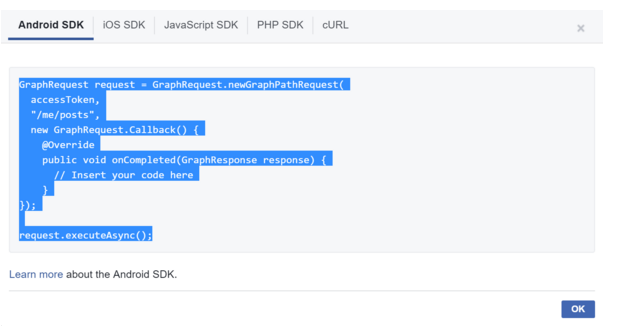
\includegraphics [width=5in,height=3in,keepaspectratio] {graphplatforms.png}      %-- include image file named as "disneychart.png" 
   \caption{Available Coding Platforms and Code Snippets in Graph API} \cite{FacebookGraphAndroid2016}
    \label{fig:graphplatforms}
\end{figure}

\begin{figure}[!htb]               %-- use [t] to place figure at top, [b] to place at the bottom, [h] for here
   \centering                    %-- use this to center the figure
   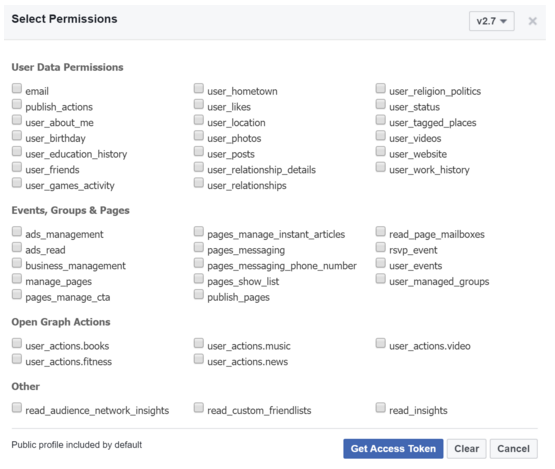
\includegraphics [width=5in,height=4in,keepaspectratio] {graphpermissions.png}      %-- include image file named as "disneychart.png" 
   \caption{Permissions in an Access Token} \cite{FacebookGraphAndroid2016}
    \label{fig:graphpermissions}
\end{figure}

\clearpage
\subsection{Facepager}
Facepager is a free and open-source tool that has gained quite a lot of interest for its simple process of collecting data through application program interfaces (APIs). Using Facepager does not require knowledge of programming because of its simple design. Presets are also available to help beginners and first time users when working with Facepager. Students and researchers commonly use this tool to gather data for projects such as for analyzing political communication on Facebook, and market analysts also make use of this tool to analyze data regarding a certain product.

Public data from Facebook, such as pages of companies or artists, enables Facepager to extract the content of the post, the number of likes, shares, and comments as well as other details provided. 

Data are collected and extracted depending on the provided object ID or Facebook page name. All these collected data are then stored in a SQLite database that could later be exported to a Comma Separated Values (CSV) file for further analysis. Each row or tuple would contain the name of the page, message, type (indicated whether it is a video, link, photo), metadata type, likes, likes count, shares count, comments count, time it was created as well as the time the post was updated.

\clearpage
\begin{sidewaystable}[ph!]   %t means place on top, replace with b if you want to place at the bottom
\centering
\caption{Comparison among the different data extraction tools.} \vspace{0.25em}
\begin{tabular}{|p{1in}|p{4cm}|p{3cm}|p{3cm}|p{3cm}|p{2cm}|p{1cm}|p{2cm}|} \hline
\centering Data Extarction Tool & Data being extracted & Extraction of Data & Input & Output & Domain & Free & Platform \\ \hline
Download Facebook Data  & Activity Log; \newline User Profile Information; \newline Messages; \newline Friend List & Facebook User Account & N/A \newline *Only requires user to log in*  &  Zip file containing html files and the media files &  Facebook & Yes & HTML\\ \hline
Graph API & Activity Log; \newline User Profile Information  & Facebook Pages or Facebook User Account & Object ID and Access Token & JSON Object & Facebook & Yes & JavaScript \newline PHP \newline Android SDK \newline iOS SDK \newline cURL \\ \hline
Facepager & Facebook resources
 & Public Facebook Pages; \newline Public Twitter pages; \newline Public youtube accounts & Object ID & Data stored in SQLLite or CSV & Facebook \newline Twitter \newline Youtube & Yes & Python\\ \hline
\end{tabular}
\label{tab:DataExtractionTool}
\end{sidewaystable}
\clearpage

%section~~~~~~~~~~~~~~~~~~~~~~~~~~~~~~~~~~~~~~~~~~~~~~~~~~~~~~~~~~~~~~
\section{Text Understanding Tools}
Text understanding is the process of inferring the intended meanings of text made in natural language, such as greetings, commands, or messages. It consists of (1) reading texts that were formed in natural language; (2) determining the implicit and explicit meaning of each element, including words, phrases, sentences, and paragraphs; and (3) making inferences based on the implicit and explicit properties of these texts \cite{ZhangLecun2015}.

Text understanding tools are relevant in this research as a means of interpreting the textual contents extracted from Facebook. The text understanding tools reviewed in this study are the following:
\begin{enumerate}
\item FastText \cite{FastText2016, Techcrunch2016}
\item DeepText \cite{DeepText2016}
\item Google Cloud Natural Language API \cite{GoogleAPI2016}
\item Stanford CoreNLP \cite{Manning14thestanford}
\end{enumerate}

Table \ref{tab:TextUnderstandingTool} shows a comparison of these text understanding tools.

\subsection{FastText}
FastText is an open-source library for building text representation and classification \cite{FastText2016}. It combines a number of language processing and machine learning concepts introduced in recent years, such as bag of n-grams and subword information. Different concepts are employed for two main purposes: efficient text classification, and learning word vector representations.

The bag of n-grams process is fast because it focuses more on the occurrences of a word as opposed to word order \cite{Techcrunch2016}. Words are represented in a multidimensional space, and linear algebra is used to calculate the relationship between a query and a categorized set of words. Via this method, a problem which is \textit{qualitative} in nature-- text analysis-- becomes qualitative through the addition of statistics. Essentially, this enables fastText to be faster than traditional deep learning methods. \figref{fig:FastText} shows a comparison between fastText and other text representation libraries. 

\begin{figure}[!htb]               %-- use [t] to place figure at top, [b] to place at the bottom, [h] for here
   \centering                    %-- use this to center the figure
   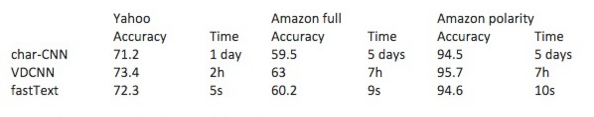
\includegraphics {FastText.png}      %-- include image file named as "disneychart.png" 
   \caption{A comparison between fastText and deep learning-based methods.}
    \label{fig:FastText}
\end{figure}

FastText is not restricted to English and can work with other languages including German, Spanish, French, and Czech \cite{Techcrunch2016}.

\subsection{DeepText}
DeepText is a ``deep learning-based text understanding engine." It can understand with near-human accuracy the textual content of several thousand posts per second \cite{DeepText2016}. It aims to help users make tasks, such as defining words or reserving plane tickets, easier.

Facebook users are composed of people with different cultures. Thus, it is important for DeepText to be able to interpret as many languages as possible. Another goal of DeepText is to better understand words in different languages using labeled data instead of traditional NLP techniques that would normally take longer processing time. In traditional NLP, the understanding part is highly dependent on stored knowledge thus requiring each word to be exactly the same for it to be understood. However, with deep learning, word embeddings could be used to get a sense of the word. According to Facebook, it is a ``mathematical concept that preserves the semantic relationship among words". By mapping words and phrases into a common embedding space, it might know which words written in different languages yield the same meaning.

\subsection{Google Cloud Natural Language API}
The Google Cloud Natural Language API offers powerful text analysis by using machine learning models that are capable of revealing the structure and meaning of text. It can extract information about entities (such as people or places) which can be found in documents, articles, or blogs. Google uses the same machine learning technology to understand and answer user questions in a Google search query.

The Natural Language API features syntax analysis, entity recognition, multi-language, and integrated REST API. Syntax analysis is the process of extracting tokens and sentences, identifying the different parts of speech, and creating dependency parse trees for each sentence. Entity recognition seeks to locate and classify entities in text into predefined categories such as person, organization, location, events, and media. The API allows analysis of text in different languages, including English, Japanese, and Spanish. And lastly, the integrated REST API allows text to be uploaded in the request or integrated with Google Cloud Storage.

The API has several methods for performing analysis on text and each level of analysis provides valuable information for text understanding. One method is [1] syntactic analysis, which consists of the following operations: (1) sentence extraction, (2) tokenization, and (3) mapping. These will help in determining the syntactic meaning of tokens and their relationships. Syntactic analysis, as shown in \figref{fig:google-syntax}, is used for analyzing and parsing text.

\begin{figure}[!htb]                %-- use [t] to place figure at top, [b] to place at the bottom, [h] for here
   \centering                    %-- use this to center the figure
   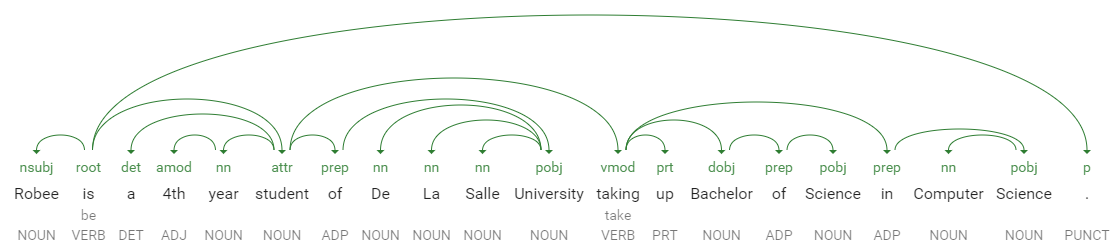
\includegraphics [width=\textwidth] {google-syntax.png}      %-- include image file named as "disneychart.png" 
   \caption{Sample output for syntax analysis}
    \label{fig:google-syntax}
\end{figure}

Another method is [2] entity analysis, as shown in \figref{fig:google-entities}. It is useful for disambiguating similar entities and providing information about each entity found in the text. The analysis returns a set of detected entities, and parameters that are in connection with the identified entities, such as the type of the entity, its relevance to the text, and positions within the text where the identity was mentioned. Each entity is ordered from highest to lowest according to their salience scores, which reflects their importance in the overall text. Scores closer to 1.0 are highly salient, while scores closer to 0.0 are less salient. 

\begin{figure}[!htb]                %-- use [t] to place figure at top, [b] to place at the bottom, [h] for here
   \centering                    %-- use this to center the figure
   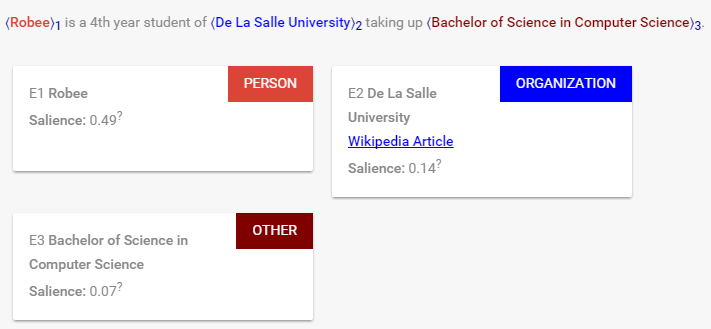
\includegraphics [width=\textwidth] {google-entities.png}      %-- include image file named as "disneychart.png" 
   \caption{Sample output for entity recognition}
    \label{fig:google-entities}
\end{figure}

\subsection{Stanford CoreNLP}
Stanford CoreNLP is a Java-based annotation pipeline framework which provides a set of natural language technology analysis tools ranging from tokenization to coreference resolution \cite{Manning14thestanford}. It supports text in different languages such as Arabic, Chinese, English, French, German, and Spanish.

Stanford CoreNLP has several options to choose from when doing syntax analysis. But before the actual syntax analysis, it must first perform two operations: (1) sentence extraction and (2) tokenization. Sentence extraction is the process of breaking down the text into separate sentences, while tokenization is the act of breaking down a sentence into tokens.

After that, the choices for syntax analysis include: (a) part-of-speech tagging (shown in \figref{fig:new-postag}), (b) named entity recognition (shown in \figref{fig:new-ner}), (c) lexical parsing (shown in \figref{fig:new-parsetree}), or (d) universal dependencies (shown in \figref{fig:new-dependencies}). Part-of-speech tagging returns the part of speech of each token; named entity recognition returns proper nouns; lexical parsing analyzes the grammatical structure of each sentence and provides a dependency tree; and the universal dependencies shows the relationship of a word to other words.

\begin{figure}[!htb]                %-- use [t] to place figure at top, [b] to place at the bottom, [h] for here
	\centering                    %-- use this to center the figure
	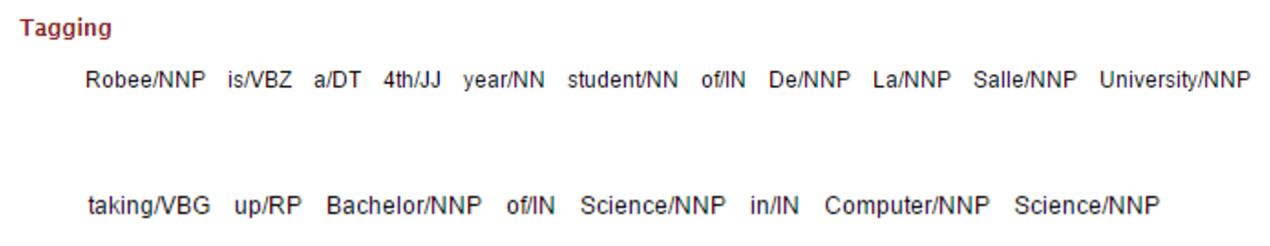
\includegraphics [width=\textwidth] {new-postag.png}      %-- include image file named as "disneychart.png" 
	\caption{Sample Part-of-speech Tagging using Stanford CoreNLP} 
	\label{fig:new-postag}
\end{figure}

\begin{figure}[!htb]                %-- use [t] to place figure at top, [b] to place at the bottom, [h] for here
	\centering                    %-- use this to center the figure
	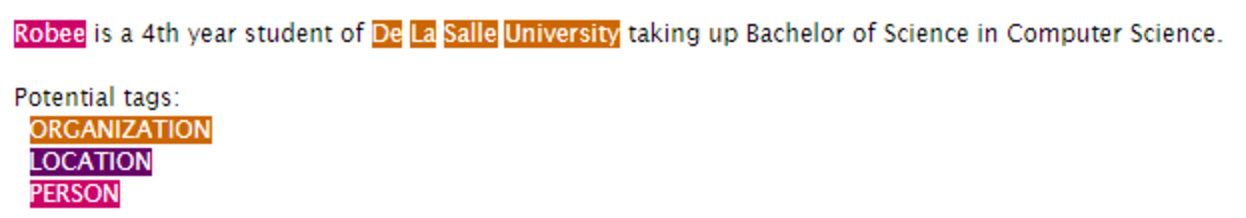
\includegraphics [width=\textwidth] {new-ner.png}      %-- include image file named as "disneychart.png" 
	\caption{Sample Named Entity Recognition using Stanford CoreNLP} 
	\label{fig:new-ner}
\end{figure}

\begin{figure}[!htb]                %-- use [t] to place figure at top, [b] to place at the bottom, [h] for here
	\centering                    %-- use this to center the figure
	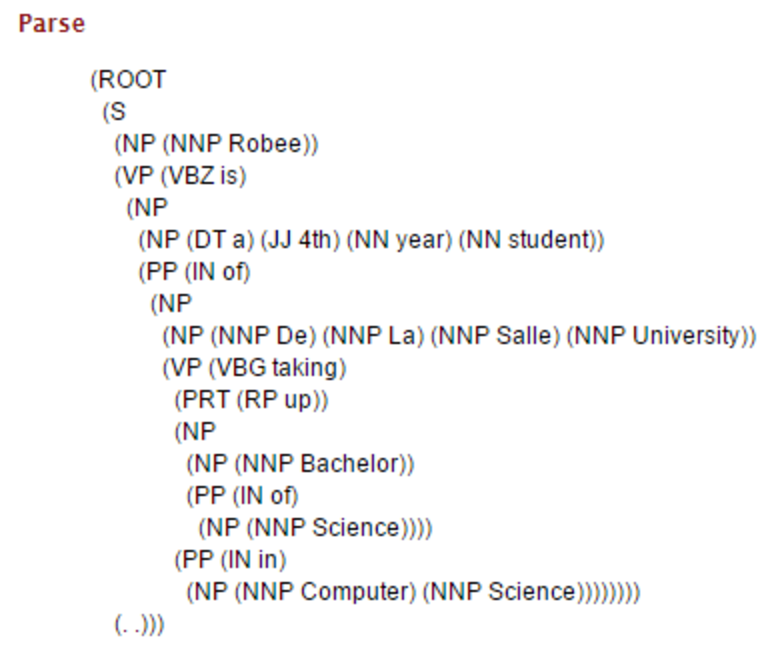
\includegraphics{new-parsetree.png}      %-- include image file named as "disneychart.png" 
	\caption{Parse Tree Output by Stanford CoreNLP} 
	\label{fig:new-parsetree}
\end{figure}

\begin{figure}[!htb]                %-- use [t] to place figure at top, [b] to place at the bottom, [h] for here
	\centering                    %-- use this to center the figure
	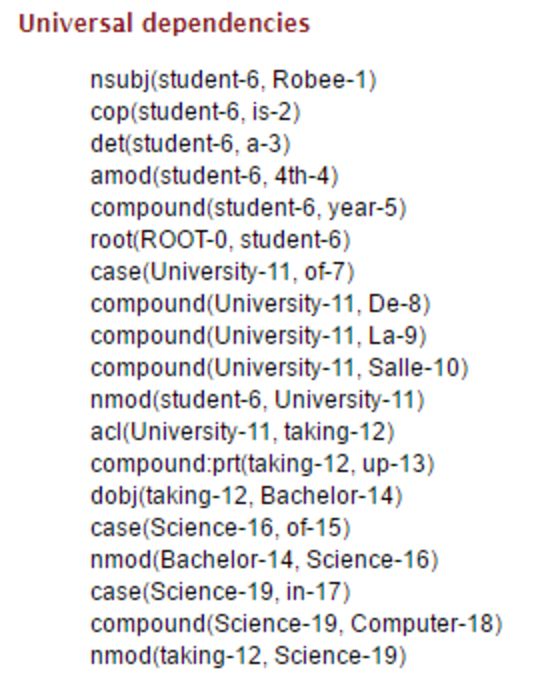
\includegraphics{new-dependencies.png}      %-- include image file named as "disneychart.png" 
	\caption{Universal Dependencies Output by Stanford CoreNLP} 
	\label{fig:new-dependencies}
\end{figure}

\clearpage
\begin{table}[ph!]   %t means place on top, replace with b if you want to place at the bottom
\centering
\caption{Comparison of the text understanding tools.} \vspace{0.25em}
\begin{tabular}{|p{1in}|p{1.5in}|p{1.5in}|p{1in}|} \hline
\centering Text Understanding Tool & Learning Process & Processes Available & Languages Supported \\ \hline
FastText & You have to train it yourself & Classification of posts & English, German, Spanish, French, and Czech \\ \hline
DeepText & Used FBLearner Flow and Torch for model training. & Entity recognition, General classification about the posts, extracting intent, and sentiment analysis & More than 20 languages \\ \hline
Google Cloud Natural Language API & Pre-trained & Entity recognition, Sentiment analysis, and Syntax analysis & English, Spanish, and Japanese \\ \hline
Stanford CoreNLP & Pre-trained & Arabic, Chinese, English, French, German, and Spanish & Part-of-Speech Tagger, Named Entity Recognition, Parser, Sentiment Analysis, Coreference, Universal Dependencies, Lemmatizer \\ \hline
\end{tabular}
\label{tab:TextUnderstandingTool}
\end{table}

%section~~~~~~~~~~~~~~~~~~~~~~~~~~~~~~~~~~~~~~~~~~~~~~~~~~~~~~~~~~~~~~
\section{Story Generation Systems}
Story generation systems output a complete story of a certain genre given a (usually) unique set of inputs. The following story generation systems are reviewed in three aspects - the different inputs accepted and the output generated; and the process of planning the story:
\begin{enumerate}
\item Novel Writer System \cite{Gervas2012, Gervas2009, MendezGervasDeleon2014, LaclaustraLedesmaMendezGervas2014}
\item TALE-SPIN \cite{Gervas2009, Mawhorter2013, Meehan1977}
\item Picture Books \cite{SolisSiyTabiraoOng2009, angenhancing, picbooks4}
\item Learning To Tell Tales \cite{McIntyreLapata2009}
\end{enumerate}

Table \ref{tab:StorytellingSystems} shows a comparison among these story generation systems.

\subsection{Novel Writer System (1973)}
The first ever storytelling system was the Novel Writer System developed by Sheldon Klein. The system was recorded to have generated 2100-word murder-mystery stories in less than 19 seconds \cite{Gervas2012}. It uses a microsimulation model in which the behavior of each character and events were ruled by probabilistic rules that continuously changes the story \cite{Gervas2009}.

The user has to provide the character traits of the murderer/s and the victim/s with additional traits that describe their relationships with each other, their tendency to commit violence or sex, and the description of the setting in which the story will take place \cite{Gervas2012,  MendezGervasDeleon2014, LaclaustraLedesmaMendezGervas2014}. During the course of the story, some of the events causes motives to arise. Greed, anger, jealousy, and fear are possible motives for murder. The system can also generate more than one text-based story, indicating who the murderer is, why the murder was committed, and who discovered the murder incident.

The system generates stories based on two different algorithms: (1) a set of rules that indicates the possible changes from the current state of the story to the next and (2) a sequence of scenes corresponding to the type of story to be told. There are pre-defined set of rules to allow the construction of only one specific type of story.

\subsection{TALE-SPIN (1977)}
TALE-SPIN is a storytelling system that generates stories about the lives of  woodland creatures developed by James Meehan \cite{Gervas2009}. It uses character simulation as a method in creating stories \cite{Mawhorter2013}.

The user chooses the traits and morals of the characters as well as the problem they will be facing \cite{Gervas2009, Meehan1977}. As the story progresses, new characters and items will be added as needed \cite{Meehan1977}. Relationships between the character may also arise to competition, dominance, familiarity, among others \cite{Gervas2009}. The system then generates a story containing the events that are to happen in order to solve the problem.

The story has three main components: (1) the problem solver, (2) the goal, and (3) the sub-goals and actual events \cite{Meehan1977}. TALE-SPIN generates stories by combining both backward and forward chaining \cite{Meehan1977}. Forward chaining is expounding on the available data to be able to extract more data until the end goal is obtained, while backward chaining is described as working backward from the given goal/s, tracking down events that will yield the solution to the problem.

\subsection{Picture Books (2008-2015)}
Picture Books 1-4 is a series of existing automated story generation systems which use picture elements (setting, characters and items) as inputs from children in producing a fable-like text-based story. Stories are generated using Natural Language Generation (NLG) techniques. The stories to be generated follow the plot structure of exposition, rising action, climax and resolution.

The architectural design of Picture Books 1 is composed of three modules: the picture editor, the story planner and the sentence generator. The picture editor starts after the user chooses the setting of the story and the selection of characters and items come right after choosing the setting. The story planner module is subdivided into two modules: the story content planner and the story organizer. The story content planner chooses a theme based on the setting and items. The story organizer arranges and organizes the events of the story in an organized manner for the user. The result of this will be a story tree that will be used in the next module.  The sentence generator module is again subdivided into two modules: the sentence planner and realizer. The sentence planner converts the story tree from the story organizer to sentence templates. The realizer then uses the SimpleNLG realiser which is an open source Java class library in converting the sentence templates given by the sentence planner to the actual sentences that made up the story. The final output of the realizer includes the story title and the story itself.

Picture Books 2 targets a slightly older age group comprising of children aged six to eight years old \cite{ang2010generating}. It creates a more creative environment through depicting stories in a sequence of scenes through the given images and characters provided. The new environment required new semantic relations to be added to define the concepts dealing with movements and positioning of the objects in the story. It is capable of developing three or more scenes portraying various scenes in the intended story where in the characters exhibit three traits assigned by the system which helps depicts the story to the children. The system structure is similar to Picture Books 1 starting with the story editor module which initializes the environment for the user. The story planner module experienced changes as it aims to impart a moral lesson to the user with the use of the character's actions. It is comprised of three modules, mainly the theme formulator, setting formulator, and event generator. The theme formulator identifies the background, character and objects present in the scene and formulates a theme defining the character trait that it lacks for further development. The setting formulator focuses on describing the location and time the story takes place which is identified through a grid placed in the scene. Events generation involves the conceptual relations on the specified theme. Lastly, the sentence planner transforms the sequence of conceptual relations using character goals into readable sentences which involves aggregation, lexicalization and referencing.

In Picture Books 4, the system automatically generates stories based on pictures or stickers the children puts on the scene \cite{picbooks4}. Similar to Picture Books 2, it focuses on children from six to eight years old. It has the capability of generating stories consisting of single to multiple scenes, and can generate stories with a single character or with multiple characters, however, it focuses more on developing stories with multiple characters by incorporating interaction between them. Unlike Picture Books 1 and 2, which only caters one type of interaction, character-to-object, and character-to-character interaction, respectively, Picture Books 4 caters to both types of interaction and two additional types of interaction which are the verbal interaction and non-verbal interaction. The system uses both character-centric and author-centric approaches. The character-centric approach allows characters to have their own individual goals and pursue these goals in a way that is consistent with their personality and desires, while the author-centric approach makes sure that the entirety of the story revolves around the main topic. The system has three modules that were adapted from previous Picture Book systems. 

\subsection{Learning To Tell Tales (2009)}
Learning To Tell Tales is a data-driven approach in storytelling \cite{McIntyreLapata2009}. The user provides the topic that may come in the form of phrase or sentence and the desired length of the story. The output is a text-based story generated after looking in the knowledge base containing the topic.

The system conceptualizes the story generation process as a tree after consulting the knowledge base. The story tree \figref{fig:storytree} has different levels which represent the number of sentences to be generated in the output. Additionally, each sentence in the tree has their own score. To generate a story, the system traverses the tree and chooses the node with the highest score. The system also uses two different searching methods: (1) searching for the best story and (2) searching for the most suitable sentences that can be gathered from the knowledge base.

\begin{figure}[!htb]                %-- use [t] to place figure at top, [b] to place at the bottom, [h] for here
   \centering                    %-- use this to center the figure
   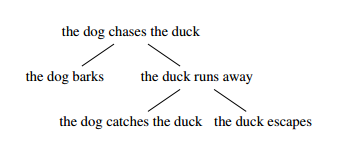
\includegraphics{storytree.png}      %-- include image file named as "disneychart.png" 
   \caption{Example Story Tree} \cite{McIntyreLapata2009}
    \label{fig:storytree}
\end{figure}

There are four modules in order to generate a story: (1) content planning, (2) sentence planning, (3) surface realization, and (4) story ranking. First, all the possible verb-subject, verb-object, verb-adverb, and noun-adjective relations related to the topics are extracted from the corpora stored in the knowledge base and each of these verbs will have a score. Second, the system must combine each of them to form a sentence. The grammar rules will act as a template. Third, the sentences will undergo surface realization which fixes the grammar of each sentence. Lastly, the system performs a story ranking to know whether the story generated is interesting and coherent.

\clearpage

\begin{sidewaystable}[ph!]   %t means place on top, replace with b if you want to place at the bottom
\centering
\caption{Comparison among the different story generation systems.} \vspace{0.25em}
\begin{tabular}{|p{1in}|p{2cm}|p{2cm}|p{2cm}|p{2cm}|p{2cm}|p{2cm}|p{2cm}|p{2cm}|} \hline
\centering Story Generation System & Genre & Target & Theme & Input & Output & Approach & Goal \\ \hline
Novel Writer System & Murder & Not specified & Weekend party & Murderer/s \newline Victim/s \newline Description of Setting & Text-based story & Rule-based & No\\ \hline
TALE-SPIN & Aesop's Fable-like stories & Not specified & Not specified & Initial Setting \newline Traits or morals of characters \newline Goal & Text-based story & Not Specified & Yes \\ \hline
Picture Books & Fable & Children (age 4 to 6) & Not specified & Settings \newline Character \newline Items & Text-based story & Author-centric \newline Character-centric & No \\ \hline
Learning To Tell Tales & Not specified  & Young Children  & Depends on the gathered information & Topic \newline Length of Story & Text-based story (based on the length specified by the user) & Knowledge-based reasoning & No \\ \hline
\end{tabular}
\label{tab:StorytellingSystems}
\end{sidewaystable}
\clearpage

%section~~~~~~~~~~~~~~~~~~~~~~~~~~~~~~~~~~~~~~~~~~~~~~~~~~~~~~~~~~~~~~
\section{Social Networking Sites}
Social networking sites (SNS) are popular tools for social interaction as well as information exchange between individuals \cite{HughesRoweBateyLee2012}. They serve as virtual communities which allow people to connect and interact with each other on a  particular subject, or to just ``hang out'' together online \cite{CheungChiuLee2011}.

The social networking sites reviewed here are Facebook and Twitter.

\subsection{Twitter}
Twitter is commonly referred as a micro-blogging website. This is a combination of instant messaging and blogging that allows users to post or send a short message, but is limited to 140 characters, called ``tweets'' \cite{Crymble2010}. In 2010, Twitter's population grew to 175 million registered users from 30 million users early that year \cite{Rao2010}. Registered users can read and post tweets, retweet other's tweet, and follow other users or industry figures for updates, while unregistered users can only read tweets from public accounts.

Twitter has become popular in today's society for several reasons. It is one of the first sites to introduce the \textit{following} and \textit{followers} concepts that appeal to the audience as they can easily follow or unfollow other users. It is also one of the most simple social media sites to use because of its simplicity and easily navigable interface. In addition, Twitter allows users to easily share information.

However, Twitter has some downsides. First, there is no system of accuracy as users can just say about anything. Second, users are limited to 140 characters, which means, they may not be able to explain themselves or their thoughts in detail. Many tweets involve either a use of  ``(con't.)'' and/or a reply to the own tweet to signify a chain of tweets that are altogether expressing a single thought. And lastly, Pear Analytics, a firm that specializes in marketing analytics, conducted a study that categorized tweets into 6 areas - News, Spam, Self-Promotion, Pointless Babble, Conversational and Pass-Along Value. They found out that 40.55\% of the tweets in the gathered sample fit into the category of Pointless Babble, followed by a 37.55\% in conversational \cite{PearAnalytics2009}.

\subsection{Facebook}
Facebook is the most active SNS today. It consists of multiple avenues of social interactions and billions of page views, with more than 21 million users as of 2007 \cite{EllisonSteinfieldLampe2007} and has dramatically increased to almost one billion users worldwide as of 2013 \cite{FarahbakhshHanCuevasCrespi2013}. The comScore Media Metrix Multi-Platform conducted a study in 2015 showing a huge gap between other social networks and Facebook for being the most accessed site for millennials as shown in \figref{fig:snsdemographics} below. According to Dave Chaffey \citeyear{Chaffey2016}, Facebook continues to dominate the social landscape, leading number one on social media platforms around the world.

\begin{figure}[!htb]                %-- use [t] to place figure at top, [b] to place at the bottom, [h] for here
	\centering                    %-- use this to center the figure
	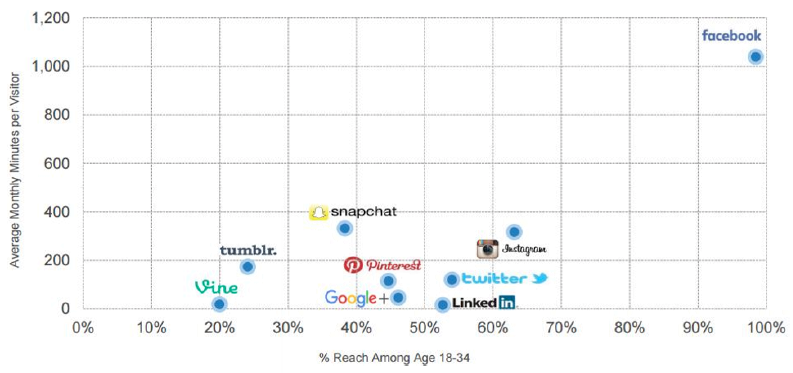
\includegraphics [width=\textwidth]{snsdemographics.png}      %-- include image file named as "disneychart.png" 
	\caption{Millennial Demographics in Social Media Platforms } \cite{Chaffey2016}
	\label{fig:snsdemographics}
\end{figure}

Facebook is a convenient and open social media platform that welcomes not just individuals but also companies and organizations to communicate and interact with one another. Westlake \citeyear{Westlake2008} states that ``Facebook develops technologies that facilitate the spread of information through social networks allowing people to share information online the same way they do it in the real world''. It promotes interactions between users, through simple status updates, posts, or shares, and enables users to inform others about their whereabouts and actions.

In Facebook, users are required to create visible profiles providing their name, gender, date of birth and email address. In addition to that, more information such as contact information, personal interests, background information and favorites (books, movies and music) can also be added to the profile at the discretion of the user \cite{NadkarniHofmann2012}. Posting information about their interest enables others to get a grasp of one's characteristics or personality \cite{FarahbakhshHanCuevasCrespi2013}. Derek Coles \citeyear{Doughty2015} said that ``Facebook is the modern way of not being on your own'' as it also allows you to interact and meet people you don't know and enables people to discuss topics with common interests. 

A study by Ashwini Nadkami and Stefan G. Hofmann \citeyear{NadkarniHofmann2012}, showed that people tend to stay online and use Facebook because posting in Facebook allows self-promotion and influences one's self-esteem and self-worth. Self-esteem and self-worth are affiliated with the sense of belonging in the society or a acceptability to a group, which, according to Nadkami \& Hoffman, can be measured by the number of likes and comments received on one's share or post or a simple act like being tagged in a group picture. The study concluded that ``Facebook creates an environment where information is shared proactively because of the site's influence on a  user's need for popularity'' \cite{NadkarniHofmann2012}.

%section~~~~~~~~~~~~~~~~~~~~~~~~~~~~~~~~~~~~~~~~~~~~~~~~~~~~~~~~~~~~~~
\section{Knowledge Base}
According to the American Heritage Dictionary (2011), a \textit{knowledge} base is a collection of data organized in a form that facilitates analysis by automated deductive processes. It can be perceived as an expert system \cite{mars1995towards}. It uses a \textit{knowledge representation language} for expressing rules and/or objects.

The different knowledge base systems reviewed in this section are as follows:
\begin{itemize}
\item Cyc \footnote{OpenCyc. http://www.opencyc.org/} \cite{cyc1999, cycinferencing1994};
\item WordNet \footnote{WordNet. https://wordnet.princeton.edu/}; and
\item ConceptNet \cite{LiuSingh2004}.
\end{itemize}

Table \ref{tab:KnowledgeBase} shows a comparison among these knowledge base systems.

\subsection{Cyc}
Cyc is an artificial intelligence project that aims to collate and assemble a complete knowledge base of everyday common sense knowledge that humans inherently have \footnote{Cyc. http://psych.utoronto.ca/users/reingold/courses/ai/cyc.html}. This project is undertaken with the goal of enabling applications that use AI to perform reasoning that can be considered humanlike.

Cyc's knowledge base consists of data from news and magazine articles, encyclopedia entries, advertisements, and more. Cyc's knowledge base is represented as a directed graph containing the following:
\begin{enumerate}
	\item Constants - terms that people understand;
	\item Variables - case-sensitive unique identifiers;
	\item Predicates - terms to represent relation types;
	\item Formulas - expressions;
	\item Logical connectors - and, or, not, implies;
	\item Quantifiers - forAll, thereExists;
\end{enumerate}

\figref{fig:cyc} shows an excerpt of Cyc's knowledge base. Fido (variable) is a (predicate) dog (constant), for example.

\begin{figure}[!htb]                %-- use [t] to place figure at top, [b] to place at the bottom, [h] for here
	\centering                    %-- use this to center the figure
	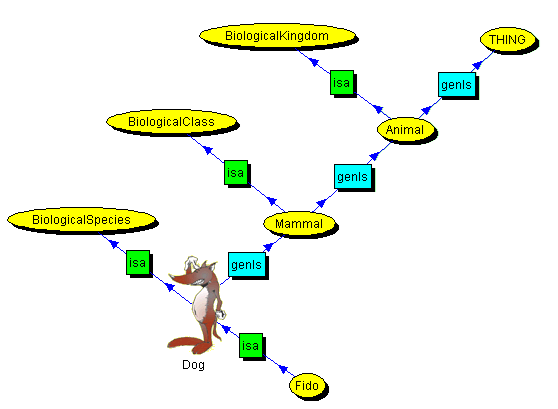
\includegraphics {cyc.png}      %-- include image file named as "disneychart.png" 
	\caption{An excerpt of Cyc's knowledge base, showing common sense knowledge about a dog named Fido.}
	\label{fig:cyc}
\end{figure}

Parts of the project were released to the public as OpenCyc, which provides an API, RDF redpoint, and data dump, all open-source \footnote{OpenCyc. http://www.opencyc.org/}. As of OpenCyc 2.0, the knowledge base contains 239,000 concepts and 2,093,000 facts, and can be browsed on the OpenCyc website. The CycL and SubL interpreter (the program that allows you to browse and edit the database as well as to draw inferences) is released free of charge, but only as a binary, without source code. It is available for Linux and Microsoft Windows.

Cyc also contains an inference engine -- that is, a computer program that derives answers from a knowledge base \footnote{Cycorop. http://www.cyc.com/overview-cyc-inferencing/}. The Cyc inference performs general logical deduction, used for reasoning.

\subsection{WordNet}
WordNet  \footnote{WordNet. https://wordnet.princeton.edu/} is a large lexical database of English words. A lexical database is a database of words and information about those words; in other words, a lexical database is a dictionary that is easily machine-readable according to The Free Dictionary \footnote{The Free Dictionary. http://www.thefreedictionary.com/}. In particular, WordNet is a database of words, primarily nouns, verbs, and adjectives, grouped into synonym sets, or ``synsets''. Rather than simply words, however, WordNet contains specific ``senses'' of words (a ``sense'' is a distinct meaning that a word can assume). These senses are linked to each other by semantic relations such as synonymy and ``is-a'' hierarchical relations (e.g. ``dog is a mammal'').

As of WordNet 2.0, the database contains around 200,000 word senses \cite{LiuSingh2004}. It is praised for being easy to use. As a simple semantic network with words at the nodes, it can be readily applied to textual input for purposes of getting more relevant results from a simple query, or determining semantic similarity between words.

\subsection{ConceptNet}
ConceptNet is a free common sense knowledge base and NLP toolkit developed by Hugo Liu and Push Singh \citeyear{LiuSingh2004}. Its information is based from the Open Mind Common Sense (OMCS) database. OMCS is an artificial intelligence project based on the Massachusetts Institute of Technology (MIT) Media Lab, and its goal is to create and maintain a large common sense knowledge base from the contributions of many people. In comparison to Cyc and WordNet, therefore, ConceptNet's knowledge base was filled in most part by the general public, rather than hiring a lot of knowledge engineers.

Common sense knowledge is knowledge that is inherent in most humans, enabling us to, for example, determine that a lemon is sour, a doorknob needs to be turned in order to open a door, or even why the sentence, ``I got fired from my job today,'' contains a negative connotation. 

ConceptNet's semantic network is expressed as a directed graph whose nodes are concepts which have atomic meaning (such as words like ``chair'', or phrases such as ``wake up''). These nodes are connected to each other by common sense knowledge about them. For example, ``waking up in the morning'' includes ``yawning'' and ``checking messages'' as its subevents as shown in \figref{fig:conceptnet}

\begin{figure}[!htb]                %-- use [t] to place figure at top, [b] to place at the bottom, [h] for here
	\centering                    %-- use this to center the figure
	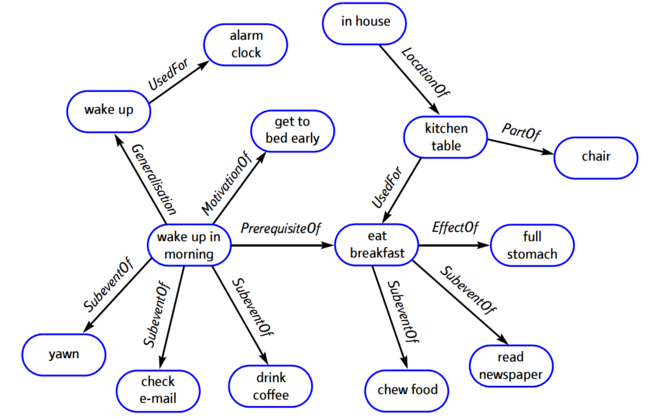
\includegraphics [width=4.5in,height=3.5in,keepaspectratio] {conceptnet.png}      %-- include image file named as "disneychart.png" 
	\caption{An example of ConceptNet's semantic network of knowledge. Concepts consist of a noun phrase along with an optional verb or prepositional phrase.}
	\label{fig:conceptnet}
\end{figure}

As of ConceptNet 5.0, there are over 3.9 million concepts, connected by 8.7 million assertions, such as ``IsA'' (``dolphin is a mammal''), ``LocationOf'' (``house is the location of kitchen table''), or ``SubeventOf'' (``chewing food is a subevent of eating breakfast'').

Through ConceptNet, it is easier to extract practical knowledge from text. This includes distinguishing between the correct definition of the word used in a context (``He ate chips with his lunch''), determining analogies, summarizing a topic, and event prediction.

\clearpage
\begin{sidewaystable}[ph!]   %t means place on top, replace with b if you want to place at the bottom
	\centering
	\caption{Comparison among the different knowledge base systems.} \vspace{0.25em}
	\begin{tabular}{|p{1.5in}|p{1.5in}|p{1.5in}|p{1.5in}|p{1.5in}|} \hline
		\centering Knowledge Base & Knowledge Objects & Relations & Content & Source of Knowledge \\ \hline
		Cyc & words & any & common sense data & magazine, news articles, encyclopedia, etc. \\ \hline
		WordNet & words & word relations like hyperonymy, hyponymy, ISA relation, antonym, etc. & English words and information about these words & \\ \hline
		ConceptNet & concepts (words or phrases) & semantic relations like LocationOf, IsA, CapableOf, SubeventOf, EffectOf, UsedFor, DesiredFor, etc. & Common sense knowledge & Open Mind Common Sense, DBPedia, Wiktionary, WordNet, OpenCyc, Verbosity, ReVerb, GlobalMind Translation, nadya.jp \\ \hline
	\end{tabular}
	\label{tab:KnowledgeBase}
\end{sidewaystable}
\clearpage

%section~~~~~~~~~~~~~~~~~~~~~~~~~~~~~~~~~~~~~~~~~~~~~~~~~~~~~~~~~~~~~~
\section{Post Classification}
A social media user's posts by themselves cannot provide a concise narrative of events in order to tell a complete life story. Story generators can be designed to utilize these events extracted from posts that users share about themselves into a life story. Before this can be achieved, however, the story generator needs to be able to classify posts based on their textual content.

With the volume of data available on social media platforms, NLP researchers have worked on putting some structure to organize text-based data to provide a more appealing interface \cite{setty2014classification}; to discover themes in disaster-related tweets \cite{syliongka2015combining}; and to find patterns and glean community sentiments in election tweets \cite{wang2012system}.

Table \ref{tab:KnowledgeBase} shows a comparison among these post classification algorithms.

\cite{DBLP:conf/ecir/KinsellaPB11} state that social media, because of its informal and brief nature, presents a unique challenge for topic classification. They note that in social media, there is a frequent reliance on hyperlinks to external sites to give context to a conversation. The paper investigated the usefulness of metadata such as those hyperlinks in order to better understand the topic of a particular post. It concluded that including object metadata at all, not necessarily hyperlink metadata, outperforms classification which is based solely on the post's original text content. 

The work of \cite{setty2014classification} involves dynamically classifying a Facebook user's news feeds into categories such as life events, entertainment and liked pages as a ``better representation of data on the user's wall". The life event posts were further classified based on their sentiments as happy, neutral and bad feelings. These studies, however, have focused on finding patterns and trends from data coming from posts and tweets of multiple users over a certain period of time. 

Choudhury and Alani \citeyear{choudhury2014personal} further noted that most research works in detecting events from social media content have focused on world events such as earthquakes and elections, and entertainment news. Focusing their own efforts on individuals, they detect common personal life events from Twitter to identify those that are interesting and important and can therefore be used to form part of a personal digital story book. They identified five events in a person's life as being the most important: [1] graduation, [2] marriage, [3] new job, [4] having a newborn child in the family, and [5] undergoing surgery. They also used related words to help find tweets that correspond to those events.

\clearpage
\begin{sidewaystable}[ph!]   %t means place on top, replace with b if you want to place at the bottom
	\centering
	\caption{Comparison among the different works regarding post classification and life story detection} \vspace{0.25em}
	\begin{tabular}{|p{1.5in}|p{1.5in}|p{1.5in}|p{1.5in}|p{1.5in}|} \hline
		\centering  & Focus & Social Network & Approach & Results \\ \hline
		Kinsella, et al. \citeyear{DBLP:conf/ecir/KinsellaPB11} & Posts with hyperlinks & Facebook & Multinomial Naive Bayes & F-score: 84\% without hyperlinks; 90\% with hyperlinks \\ \hline
		Setty, et al. \citeyear{setty2014classification} & Classifying posts on news feed & Facebook & SVM, Logistic Regression & Accuracy: 93\%; Precision: 94\%; Recall: 94\% \\ \hline
		Choudhury \& Alani \citeyear{choudhury2014personal} & Detecting life events in posts & Twitter & Naive Bayes, Multinomial Naive Bayes, SVM & AUC: 77\%; Precision: 80\%; Recall: 85\% \\ \hline
	\end{tabular}
	\label{tab:KnowledgeBase}
\end{sidewaystable}
\clearpage 
 
%%%%%%%%%%%%%%%%%%%%%%%%%%%%%%%%%%%%%%%%%%%%%%%%%%%%%%%%%%%%%%%%%%%%%%%%%%%%%%%%%%%%%%%%%%%%%%%%%%%%%%
%
%   Filename    : chapter_3.tex 
%
%   Description : This file will contain your Theoretical Framework.
%                 
%%%%%%%%%%%%%%%%%%%%%%%%%%%%%%%%%%%%%%%%%%%%%%%%%%%%%%%%%%%%%%%%%%%%%%%%%%%%%%%%%%%%%%%%%%%%%%%%%%%%%%

%\footnote{Oxford Dictionary. https://en.oxforddictionaries.com}
%\footnote{The Free Dictionary. http://www.thefreedictionary.com/}

\chapter{Theorerical Framework}
\label{sec:theoreticalframewrok}

This chapter introduces and expands on the relevant concepts and theories to be used over the course of this research.

%section~~~~~~~~~~~~~~~~~~~~~~~~~~~~~~~~~~~~~~~~~~~~~~~~~~~~~~~~~~~~~~
\section{Life Stories}
A \textit{life story}, or a biography, is an account of the series of events making up a person's life according to The Free Dictionary \footnote{The Free Dictionary. http://www.thefreedictionary.com/}. An \textit{autobiography}, or a \textit{memoir}, is an account of a person's life written by themselves according to Oxford Dictionary \footnote{Oxford Dictionary. https://en.oxforddictionaries.com}. An \textit{event} is anything that happens, especially one of importance according to Oxfor Dictionary \footnote{Oxford Dictionary. https://en.oxforddictionaries.com}.

The following sections describe the different elements of a story, and the linguistic concerns surrounding the expression of these elements. 

\subsection{Elements and Structure of a Story}
A story has a beginning, middle, and end portion (Pacis, personal communication, October 12, 2016). Failure to provide any of these parts renders a story incomplete and disinteresting. The linear structure of a story, as shown in \figref{fig:linearstructure}, is taken from (Pacis \& Gojo-Cruz, as cited by \cite{Chua2016}) as well as from (Hancock, 1994 as cited in Types of Plot, 2010), who states that a plot is a ``sequence of events that occurs to characters in situations in the beginning, middle, and end of a story.''

\begin{figure}[!htb]                %-- use [t] to place figure at top, [b] to place at the bottom, [h] for here
   \centering                    %-- use this to center the figure
   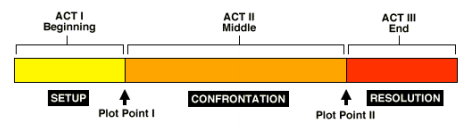
\includegraphics [width=\textwidth] {linearstructure.png}      %-- include image file named as "disneychart.png" 
   \caption{A model of the linear structure of a story.}
    \label{fig:linearstructure}
\end{figure}

As seen in \figref{fig:linearstructure}, events, details, or plot points, may occur that separate the beginning from the middle, and the middle from the end. 

\begin{figure}[!htb]                %-- use [t] to place figure at top, [b] to place at the bottom, [h] for here
   \centering                    %-- use this to center the figure
   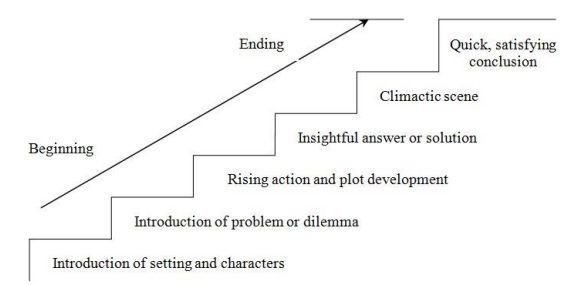
\includegraphics [width=\textwidth] {storystructure.png}      %-- include image file named as "disneychart.png" 
   \caption{The story structure used in Picture Books, which tells the (fictional) story of a child who is disobedient.}
    \label{fig:storystructure}
\end{figure}

Stories for children, such as those generated by the Picture Books story generation system \cite{SolisSiyTabiraoOng2009}, follow the structure of Machado (2003, as cited in \cite{SolisSiyTabiraoOng2009}) which consists of the introduction; a problem; rising action; solution; and climax. \figref{fig:storystructure} illustrates the structure of Picture Books 1's stories.

Some of the elements present in Picture Books' stories are only necessary in the case of fictional stories, while some will still be necessary, such as having a beginning and an end. Life stories, which are a different type of story from children's stories or other fictional stories, follow a different pattern. According to Youse \citeyear{Youse2005}, there are ten (10) necessary elements present in a life story. These are:
\begin{enumerate}
\item \textbf{Birthday and birthplace}. The story should be able to indicate when and where a person's life started.
\item \textbf{Family members}. Was this person the eldest in a few children? Did he/she eventually take a spouse and sire any children? Did he/she have notable relatives?
\item \textbf{Childhood and education life}. Early achievements or stories that happened early on in this person's life may have had an impact later on in his/her life.
\item \textbf{Hobbies, interests, and notable activities}. This is present for the reader to be able to get an initial impression of this person. Do the person's hobbies or activities make them more interesting? Do they relate to other aspects of their life? Being able to craft interesting stories is important in this research, and describing a person's hobbies is one part of it.
\item \textbf{Photos or likenesses}. Providing a likeness of the person will complete the impression the reader has about that person.
\item \textbf{Anecdotes}. Interesting stories about this person as told by others, that makes this person more interesting.
\item \textbf{Career} (if the person is old enough to have had one). Is their work a big reason on why a story is being told about them? Does their career relate to their interests, or past experiences? Did they make significant contributions to mankind by doing their job?
\item \textbf{Reason for fame}. At what point in their life did this person become noteworthy or famous, and why?
\item \textbf{Later life} (if the person is deceased). Did they continue their work and/or contributions to mankind later on in their life? Were they honored for their achievements?
\item \textbf{Death} (if the person is deceased). When and where did they die, and under what circumstance? Was there anything unusual or significant about their death? For example, U.S. Presidents Thomas Jefferson and John Adams both died on 4 July 1826; 4 July being the American Independence Day.
\end{enumerate}

All, or most of, these elements should be present in a life story. Such a story structure can be found by perusing articles about a person's life (e.g. Miriam Defensor Santiago). However, some elements (such as numbers 7-10 in the list above) are not possible to put into a person's life story because they may not be old enough. For these ones, concern should be put into ensuring that the story ends in a satisfying manner despite the missing details.

%section~~~~~~~~~~~~~~~~~~~~~~~~~~~~~~~~~~~~~~~~~~~~~~~~~~~~~~~~~~~~~~
\section{Facebook}

\subsection{Facebook Content}
Facebook contains a lot of data ranging from texts to photos and to videos. It contains numerous of varying stories, facts and events from users all around the world. Each user has the ability to post any content they prefer to which can be categorized into 13 categories, as shown in \figref{fig:facebookcontent}.

\begin{figure}[!htb]                %-- use [t] to place figure at top, [b] to place at the bottom, [h] for here
   \centering                    %-- use this to center the figure
   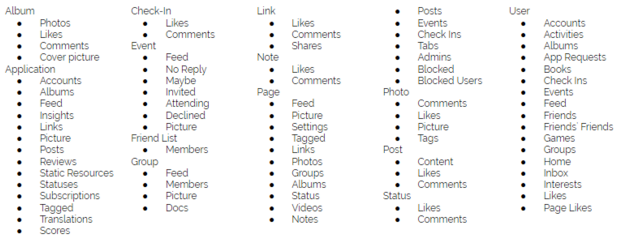
\includegraphics [width=\textwidth] {facebookcontent.png}      %-- include image file named as "disneychart.png" 
   \caption{Facebook content categorized into 13 categories.}
    \label{fig:facebookcontent}
\end{figure}

\subsection{Facebook Components}
Facebook is comprised of eight different components namely: [1] News Feed, [2] Friends, [3] Timeline, [4] Likes, Comments, and Shares, [5] Messages and Inbox, [6] Notifications, [7] Groups and [8] Statuses or Posts. In this section, only the status or posts component will be discussed since these will be the focus of the research.

\subsubsection{Status or Posts}
In 2013, Facebook has added a new structured status update feature allowing users to specify what they are feeling, watching, listening, playing, celebrating, among others \cite{darwell}. Those which we will be using for event classification in this research are the following:

\begin{enumerate} [label=\alph*.]
\item Celebrating - Shows what the user is remembering at the time of posting.
\item Travelling To - Tells where the user is travelling at the time of the status update. The user can include the Facebook page of the location he/she is currently travelling to or he/she can simply include the location if there is no Facebook page for that.
\item Eating - Tells what food the user is consuming.
\item Drinking - Tells what beverage the user is drinking.
\end{enumerate}

%section~~~~~~~~~~~~~~~~~~~~~~~~~~~~~~~~~~~~~~~~~~~~~~~~~~~~~~~~~~~~~~
\section{Data Extraction Tool}
For this research, Graph API was used for data extraction. Graph API is a low-level HTTP-based API that is primarily used to access data and information in Facebook's platform \cite{FacebookGraphAndroid2016}. It allows applications to do certain actions in Facebook such as publish updates, media files and even schedule a post. 

\subsection{Structure}
The structure of Graph API consists of three main types, namely: nodes, edges and fields. Nodes are the basic components of Facebook such as a user, page, or comment; edges are the connections between the nodes, such as the connection between a user's photo and that photo's comment; and fields are the details or information about a specific node, such as the first and last names of the user.

These nodes can be accessed through making HTTP GET requests passed to the API at graph.facebook.com or graph-video.facebook.com for video uploads. Most APIs would require access tokens which determine the permissions for secure access to Facebook APIs. Each access token contains information about the token's expiration as well as the application in which it was generated (in this case, our system).

When a user logs into Facebook through an application (or app), the app will be able to obtain an access token which allows access to the user's data on Facebook \cite{FacebookToken2013}. Logging in only accesses the basic permissions such as the public default. Additional permissions can be listed down in the scope parameter and would inform whether the user would choose to authenticate the app with the said permissions \cite{FacebookJavaScript}. The user access tokens are then automatically stored by the Facebook SDK for JavaScript. These can be retrieved through FB.getAuthResponse which obtains the access token within the received response.

\subsection{JSON File}
Once the access token with the prefered permissions is obtained, the system can access the user's Facebook data through HTTP GET requests and receive a JSON file containing the requested information from the user.  The structure of the JSON file received may vary depending on the node or edges read \cite{FacebookGraphAndroid2016}. The general form for this is:
	\{
		 ``fieldname'' : \{field-value\}, ….
	\}
	
%section~~~~~~~~~~~~~~~~~~~~~~~~~~~~~~~~~~~~~~~~~~~~~~~~~~~~~~~~~~~~~~
\section{Text Understanding}
For this research, the Stanford CoreNLP API, a service that gives access to a set of natural language analysis tools, was used. More specifically, the API's part-of-speech tagger, named entity recognizer, parser, and universerval dependencies were used to understand text. The API takes in a string as an input and its output can be viewed in four different ways, each of which was shown by the aforementioned tools.

Given the sentence, ``Robee is a 4th year student of De La Salle University taking up Bachelor of Science in Computer Science.", the API produces the results shown in \figref{fig:stanford-aner}, \figref{fig:stanford-parsingsample}, \figref{fig:stanford-parsetree2}, and \figref{fig:stanford-dependencies2}, for named entity recognition, part-of-speech tagging, parsing, and universal dependencies.

\subsection{Named Entity Recognition}
Named Entity Recognition (NER) is a process that classifies entities in the given text and categorizes them as person, organization, location, among other classifiers. The Stanford CoreNLP API determines the known entities and returns information about those entities. 

In the CoreNLP package, it has two classes, Annotation, and Annotator. Annotations are data structures that hold the results put out by Annotators. They can hold parsed data, part-of-speech tags, or named entity tags. Annotators, on the other hand, work like functions. They can parse and tokenize text and perform NER tagging on sentences. Annotations and Annotators are integrated by AnnotationPipelines, which can create sequences of Annotators. 

To construct a Stanford CoreNLP object from a given set of properties, StanfordCoreNLP (Properties props) must be used. The method creates a pipeline using the given annotators in the annotators property.

\begin{figure}[!htb]                %-- use [t] to place figure at top, [b] to place at the bottom, [h] for here
	\centering                    %-- use this to center the figure
	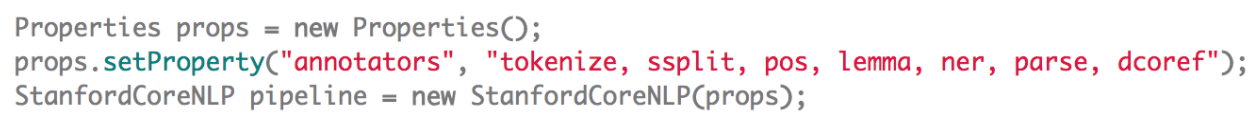
\includegraphics [width=\textwidth] {stanford-pipeline.png}      %-- include image file named as "disneychart.png" 
	\caption{Sample Code for Creating Pipeline}
	\label{fig:stanford-pipeline}
\end{figure}

The code snippet shown in \figref{fig:stanford-pipeline} creates a Stanford CoreNLP object with the following annotators: named entity recognition, part-of-speech tagging, parsing, and lemmatization. For named entity recognition, the ner annotator is used.

\begin{figure}[!htb]                %-- use [t] to place figure at top, [b] to place at the bottom, [h] for here
	\centering                    %-- use this to center the figure
	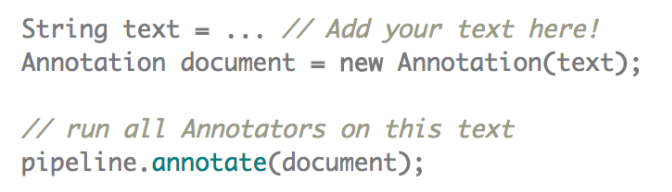
\includegraphics [width=\textwidth] {stanford-parsing.png}      %-- include image file named as "disneychart.png" 
	\caption{Sample Code for Parsing Text}
	\label{fig:stanford-parsing}
\end{figure}

After creating a Stanford CoreNLP object, the annotate(Annotation document) method is used to parse arbitrary text as shown in \figref{fig:stanford-parsing}. 

\begin{figure}[!htb]                %-- use [t] to place figure at top, [b] to place at the bottom, [h] for here
	\centering                    %-- use this to center the figure
	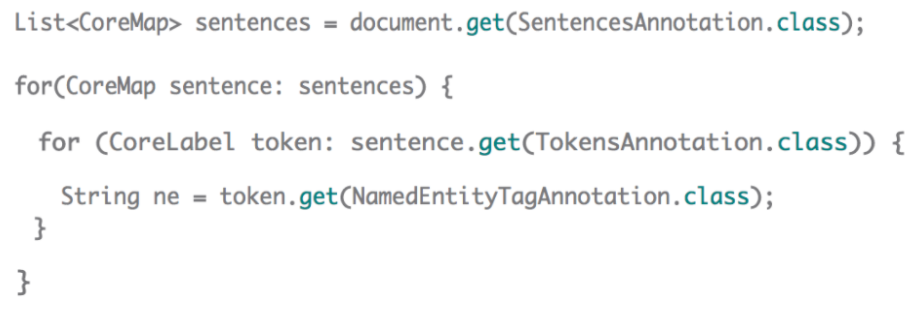
\includegraphics [width=\textwidth] {stanford-ner.png}      %-- include image file named as "disneychart.png" 
	\caption{Sample Code for Named Entity Recognition}
	\label{fig:stanford-ner}
\end{figure}

The output of the Annotators is accessed using the data structures CoreMap and CoreLabel (in \figref{fig:stanford-ner}). Entity type for each token can be retrieved using the get (NamedEntityTagAnnotation.class). 

The analysis of the online version of Stanford CoreNLP from the sample input returned a set of detected entities namely, ``Robee" and ``De La Salle University"; along with their corresponding types (shown in \figref{fig:stanford-aner}).

\begin{figure}[!htb]                %-- use [t] to place figure at top, [b] to place at the bottom, [h] for here
	\centering                    %-- use this to center the figure
	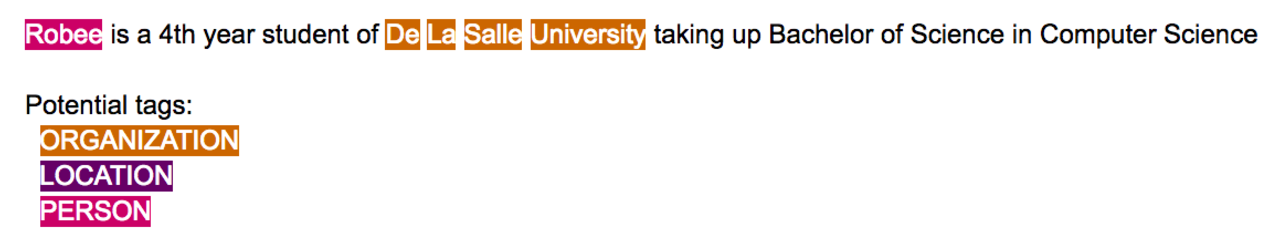
\includegraphics [width=\textwidth] {stanford-aner.png}      %-- include image file named as "disneychart.png" 
	\caption{Actual Named Entity Recognition Output by Stanford CoreNLP}
	\label{fig:stanford-aner}
\end{figure}

\subsection{Part-of-Speech Tagging}
A Part-of-Speech Tagger is a piece of software that can read text in some language, break it down into tokens, and assign a part to each token, such as \textit{noun}, \textit{verb}, or \textit{adjective}. 

For the part-of-speech tagging, the pos annotator is used to label tokens with their POS tag. 

\begin{figure}[!htb]                %-- use [t] to place figure at top, [b] to place at the bottom, [h] for here
	\centering                    %-- use this to center the figure
	
\includegraphics [width=\textwidth] {stanford-parsing-token.png}      %-- include image file named as "disneychart.png" 
	\caption{Sample Code for Getting the Part-of-Speech Tag of Each Token}
	\label{fig:stanford-parsingtoken}
\end{figure}

Part-of-speech tag of each token can be retrieved using the get(PartOfSpeechAnnotation.class) method shown in \figref{fig:stanford-parsingtoken}. A sample part-of-speech tagging using the online version of Stanford CoreNLP is shown in \figref{fig:stanford-parsingsample}.

\begin{figure}[!htb]                %-- use [t] to place figure at top, [b] to place at the bottom, [h] for here
	\centering                    %-- use this to center the figure
	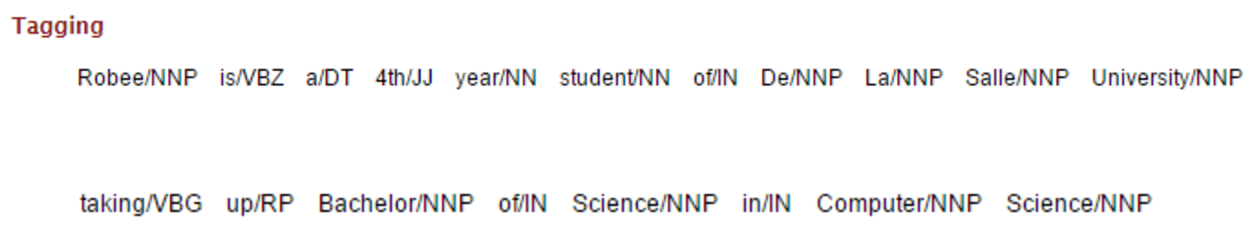
\includegraphics [width=\textwidth] {stanford-parsingsample.png}      %-- include image file named as "disneychart.png" 
	\caption{Sample Part-of-speech Tagging using Stanford CoreNLP}
	\label{fig:stanford-parsingsample}
\end{figure}

\subsection{Parsing}
The \textit{parser} annotator generates the parse tree for each sentence. It mainly analyzes the grammatical structure of sentences, for instance, determining which set of words are of the same group and which words are the subject, doer, or receiver of the action.

The sample parser returned by the online version of Stanford CoreNLP from the input is shown in \figref{fig:stanford-parsetree2}.

\begin{figure}[!htb]                %-- use [t] to place figure at top, [b] to place at the bottom, [h] for here
	\centering                    %-- use this to center the figure
	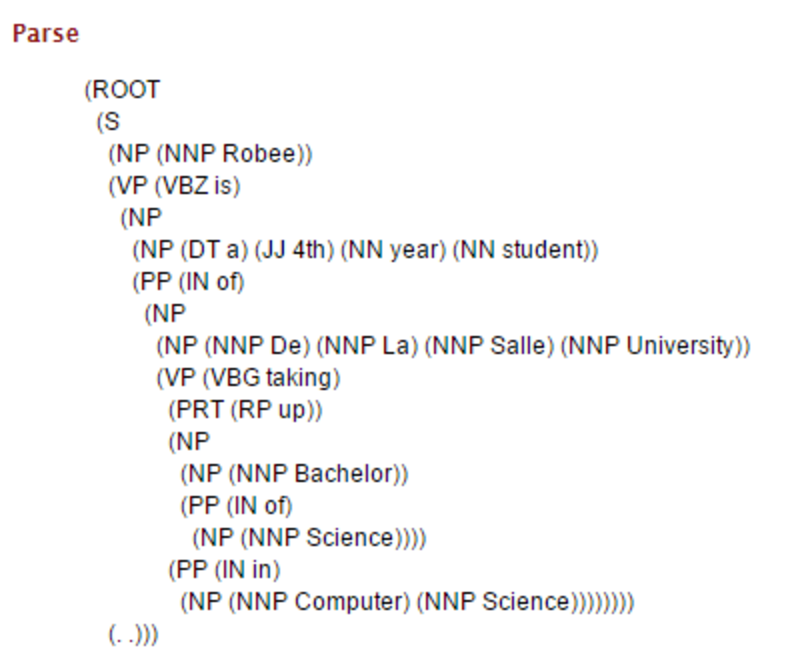
\includegraphics [width=\textwidth] {stanford-parsetree2.png}      %-- include image file named as "disneychart.png" 
	\caption{Parse Tree Output by Stanford CoreNLP}
	\label{fig:stanford-parsetree2}
\end{figure}

\clearpage
\subsection{Universal Dependencies}
The Universal Dependencies annotator generates all the possible relationships of one token to the other tokens. It mainly does the full syntactic analysis of the sentence and checks which tokens has a relationship with the others based on the probabilistic parser \cite{Manning14thestanford}. 

An example of the universal dependencies returned by the online version of Stanford CoreNLP from the input is shown in \figref{fig:stanford-dependencies2}.

\begin{figure}[!htb]                %-- use [t] to place figure at top, [b] to place at the bottom, [h] for here
	\centering                    %-- use this to center the figure
	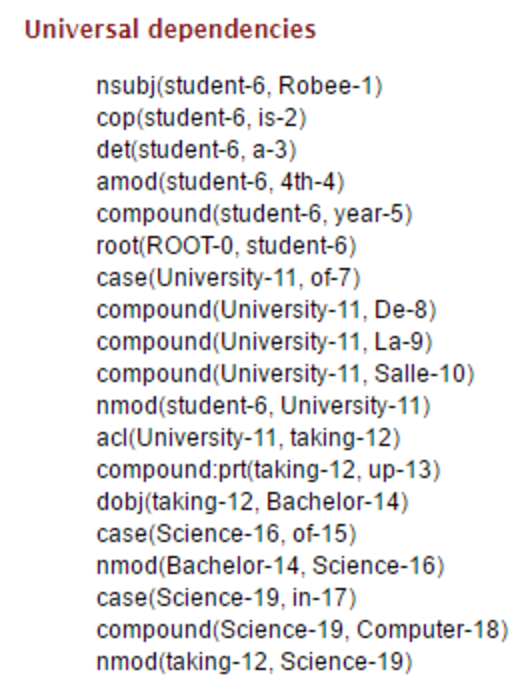
\includegraphics  [width=4in,height=6in,keepaspectratio] {stanford-dependencies2.png}      %-- include image file named as "disneychart.png" 
	\caption{Universal Dependencies Output by Stanford CoreNLP}
	\label{fig:stanford-dependencies2}
\end{figure}

\clearpage
%section~~~~~~~~~~~~~~~~~~~~~~~~~~~~~~~~~~~~~~~~~~~~~~~~~~~~~~~~~~~~~~
\section{Text Generation}
Natural language generation (NLG) is defined as the process of constructing thoughts or non-linguistic inputs into understandable English texts \cite{IndurkhyaDamerau2010, JurafskyMartin2000, ReiterDale1997}. It uses concepts stored in a knowledge base and decides how to generate text that humans can understand.

An NLG system's task is described as mapping the input data to an output text \cite{ReiterDale1997}. An NLG system must perform six different tasks that needs to be done in order to produce a final output text from the given input. The process in each task is discussed below.

\subsection{Content Determination}
During content determination, the NLG system decides what information needs to be communicated in the text from the given input \cite{ReiterDale1997}. Content must be appropriate for the reader or the user \cite{JurafskyMartin2000}. This process will create messages from the knowledge base. These messages are represented as data objects and will be passed to the next process. The whole message creation process is consists of filtering and summarizing the input data and the messages created can be expressed as entities, concepts and relations in the domain \cite{ReiterDale1997}. In \figref{fig:ContentDeterminition}, three different messages are created.

\clearpage
\begin{figure}[!htb]                %-- use [t] to place figure at top, [b] to place at the bottom, [h] for here
   \centering                    %-- use this to center the figure
   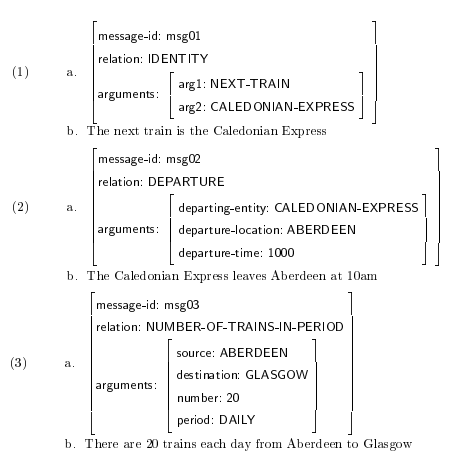
\includegraphics [width=4in,height=4in,keepaspectratio] {ContentDeterminition.png}      %-- include image file named as "disneychart.png" 
   \caption{Sample Messages} \cite{ReiterDale1997}
    \label{fig:ContentDeterminition}
\end{figure}

\subsection{Discourse Planning}
In comparison to stories having a beginning, middle and end, a message must have a structure, one which must be logical and more distinguishable than the structure used for stories\cite{ReiterDale1997}. In the process of discourse planning, the ordering and structuring of the messages produced by the content determination are done. Content determination has no knowledge of the discourse structure which the message resides nor the content of the message itself \cite{JurafskyMartin2000}.

In generating stories, the system needs to produce a multi-message output. The easiest way is to produce a message for each intended meaning, but what most cases require is the structuring of messages in an appropriate way \cite{JurafskyMartin2000}. For example: ``I have just compiled a simple C program. I have just run a single C program. The environment is configured properly.'' These three messages are individually coherent but are not joined properly.

The discourse planning process results in a tree structure. The leaf nodes represents the individual messages and the internal nodes tells how these messages are placed together and how they are related to one another. Sometimes, the internal nodes also include the discourse relations between their children. For example, as seen in \figref{fig:TreeStructureDiscoursePlanning}, the leaf node [DEPARTURE] is an elaboration of the leaf node [IDENTITY]. Later, these clusterings will have an impact in the determination of the sentence and paragraph boundaries of the final output.

\begin{figure}[!htb]                %-- use [t] to place figure at top, [b] to place at the bottom, [h] for here
   \centering                    %-- use this to center the figure
   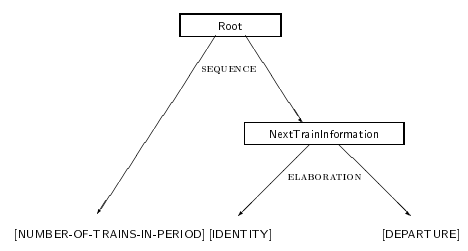
\includegraphics [width=4in,height=4in,keepaspectratio] {TreeStructureDiscoursePlanning.png}      %-- include image file named as "disneychart.png" 
   \caption{Tree Structure Returned by the Discourse Planning} \cite{ReiterDale1997}
    \label{fig:TreeStructureDiscoursePlanning}
\end{figure}

The discourse planner is composed of two main components for building the discourse structure namely: (1) Text Schemata and (2) Rhetorical Relations. 

\subsubsection{Text Schemata}
A simple method of generating text is positioning words into the templates. Another way to generate texts is to make choices based on the stored data according to the matched patterns in the system's knowledge base \cite{IndurkhyaDamerau2010}.

An observation of using the text schemata is that the texts follow a structural pattern. The schemata is represented by an augmented transition network (ATN) as shown in \figref{fig:AugmentedTransitionNetwork} which consists of states that is represented by an information that is chosen from the collection of data and transitions from one state to the other \cite{JurafskyMartin2000, IndurkhyaDamerau2010}. The transition between the states can be described as the cause followed by the effect, a sequence of events, and so on. State S0 defines the start state and State S2 defines the goal state. A loop in the states tells that there are additional information about the object, and sub-steps or side-effects of an action. 

\clearpage
\begin{figure}[!htb]                %-- use [t] to place figure at top, [b] to place at the bottom, [h] for here
   \centering                    %-- use this to center the figure
   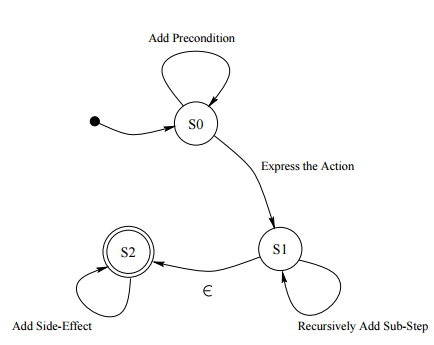
\includegraphics [width=4in,height=4in,keepaspectratio] {AugmentedTransitionNetwork.png}      %-- include image file named as "disneychart.png" 
   \caption{Augmented Transition Network (ATN)} \cite{JurafskyMartin2000}
    \label{fig:AugmentedTransitionNetwork}
\end{figure}

Using the text schemata is more flexible than directly placing words into the templates. The output was structured according to patterns of expression and add other informations extracted from the knowledge base \cite{JurafskyMartin2000}.

\subsubsection{Rhetorical Relations}
Rhetorical Structure Theory (RST), is a descriptive theory of text organization based on the relationships of two or more messages (Mann and Thompson, 1987 as cited in \cite{JurafskyMartin2000}). Some of the common RST relations are as follow \cite{JurafskyMartin2000}:
\begin{enumerate}
\item ELABORATION - This shows additional details about the content of the message. Elaboration may be in a form of:  (1) a member of a set, (2) an instance of an abstract class, (3) a part of a whole, (4) a step of a process, (5) an attribute of an object, and (6) a specific instance of a generalization.
\item CONTRAST - This shows things that, while there are some similarities between the two messages, they are still different in some other ways.
\item CONDITION - This states that something must happen in one of the messages before the situation in the other message can happen.
\item PURPOSE - One of the messages contains the goal of the other message.
\item SEQUENCE - The messages are in arranged in a sequence.
\item RESULT - One of the two messages is an outcome of the other message.
\end{enumerate}

\subsection{Sentence Aggregation}
This process organizes messages together into sentences. Based from the tree output of the Discourse Planning, the leaf nodes [IDENTITY] and [DEPARTURE] are together, so the sentence aggregation can combine the two messages into a single sentence which can be aggregated as ``The next train, which leaves at 10am, is the Caledonian Express.''. Sentence aggregation is not always required. Some of the messages can be expressed as a single sentence, but it would not result to the readability of the text \cite{ReiterDale1997}.

\subsection{Lexicalization}
In this process, the system maps the right words and phrases to convey the concepts and relations of the messages. The problem in lexicalization is the choosing of appropriate words or phrases to express the content \cite{JurafskyMartin2000}. For example, the words ``leave'' and' ``depart'' are both associated with the word ``derapture'' and the lexical selection must only choose one word to associate departure. Sometimes, lexicalization are simplified by hard-coding a single term with each entry in the knowledge base \cite{JurafskyMartin2000}. Although, this could be improved by varying the words used to express the concept or relation to obtain variety \cite{ReiterDale1997}. 

\subsection{Referring Expression Generation}
The task of creating referring expressions to identify the entities are done by the referring expression generation (REG). The Referring Expression (RE) is any noun phrase, whose task is to give identification to the objects (persons, things, or events). REG's goal is to add information to identify the entities unambiguously \cite{ReiterDale1997}. For example, in the sentence: ``The next train is the \textit{Caledonian Express. It} leaves at 10am. Many tourist guidebooks highly recommend \textit{this train}.'', the entity [CALEDONIAN-EXPRESS] from the content determination is referred to the ``Caledonian Express''; the second time to express Caledonian express is written as the pronoun ``it'' and  the use of ``this train'' to refer something that was already introduced before. REG and lexicalization are closely associated since both process chooses words and phrases to associated the domain. However, the referring expression generation needs to gather previous information to differentiate one entry from other entries. 

\subsection{Linguistic Realization}
Reiter \& Dale \citeyear{ReiterDale1997} explained the last process as applying grammar rules in order to generate a text which is syntactically, morphologically and orthographically correct. The sentence generated is syntactically correct when the grammatical arrangement of words in the sentence is correct; morphologically correct when the structure and form of words are correct; and orthographically correct when the words have correct spelling, hyphenation, capitalization, and punctuation. For example, in the sentence ``There are 20 trains each day from Aberdeen to Glasgow'', (1) the syntactic component of the linguistic realizer added the function words ``from'' and ``to" to describe the train's source and destination, (2) the morphological component of the linguistic realiser converted ``train'' to its plural form ``trains'', and (3) the orthographical component of the linguistic realizer capitalized the first word of the sentence and added a period (.) at the end of the sentence \cite{ReiterDale1997}.

\subsection{SimpleNLG}
SimpleNLG, a Java API for Natural Language Generation, is used to help write a program that can generate grammatically correct English sentences.  

\begin{figure}[!htb]                %-- use [t] to place figure at top, [b] to place at the bottom, [h] for here
	\centering                    %-- use this to center the figure
	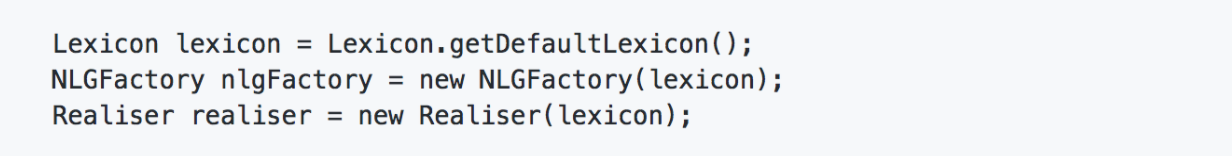
\includegraphics [width=4in,height=4in,keepaspectratio] {simplenlgA.png}      %-- include image file named as "disneychart.png" 
	\caption{SimpleNLG's lexicon, nlgFactory, and realiser}
	\label{fig:simplenlgA}
\end{figure}

Before the API can generate actual sentences, SimpleNLG lexicon, NLGFactory, and realiser are instantiated (shown in \figref{fig:simplenlgA}). Like any other natural language processing systems, SimpleNLG uses information about words from lexicons. SimpleNLG comes with a default lexicon that can be accessed via Lexicon lexicon = Lexicon.getDefaultLexicon(). NLGFactory is used to create SimpleNLG structures, and a realiser is used to transform SimpleNLG structures into text.

\begin{figure}[!htb]                %-- use [t] to place figure at top, [b] to place at the bottom, [h] for here
	\centering                    %-- use this to center the figure
	
\includegraphics [width=4in,height=4in,keepaspectratio] {simplenlgB.png}      %-- include image file named as "disneychart.png" 
	\caption{SimpleNLG's SPhraseSpec} 
	\label{fig:simplenlgB}
\end{figure}

To generate sentences, a class called SPhraseSpec is used, which is accessible through the NLGFactory, using the createClause method (shown in \figref{fig:simplenlgB}). 

\begin{figure}[!htb]                %-- use [t] to place figure at top, [b] to place at the bottom, [h] for here
	\centering                    %-- use this to center the figure
	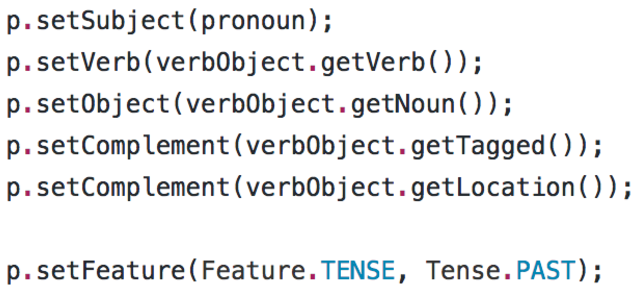
\includegraphics [width=4in,height=4in,keepaspectratio] {simplenlgC.png}      %-- include image file named as "disneychart.png" 
	\caption{SimpleNLG's SPhraseSpec methods}
	\label{fig:simplenlgC}
\end{figure}

SPhraseSpec allows for defining a sentence in terms of its syntactic constituents, which can be useful for specifying different parts of a sentence or clause, in no particular order. SimpleNLG then assembles those parts into grammatically correct sentences. The setSubject(subject), setVerb(verb), setObject(object), setComplement(complement), and setFeature(tense, tense) methods are used to define the sentence's subject, verb, object, complement, and tense respectively (shown in \figref{fig:simplenlgC}).

\begin{figure}[!htb]                %-- use [t] to place figure at top, [b] to place at the bottom, [h] for here
	\centering                    %-- use this to center the figure
	
\includegraphics [width=4in,height=4in,keepaspectratio] {simplenlgD.png}      %-- include image file named as "disneychart.png" 
	\caption{SimpleNLG's realiser}
	\label{fig:simplenlgD}
\end{figure}

Given the subject - She; verb - going; object - to the mall; tagged - none; location - none; and verb tense - past. The realiser takes in the different components of the sentence, combines them, and generates a syntactically and morphologically correct text using the code snippet shown in \figref{fig:simplenlgD}.  The resulting sentence will then result to ``She went to the mall.”.

%section~~~~~~~~~~~~~~~~~~~~~~~~~~~~~~~~~~~~~~~~~~~~~~~~~~~~~~~~~~~~~~
\section{Knowledge Base}
This section discusses the different existing knowledge bases that were used in the implementation of the system: WordNet and ConceptNet.

\subsection{WordNet}
WordNet's database provides connections among nouns and verb synsets containing words that share an underlying meaning. It contains derivational links that connect noun and verb senses (e.g. travel - traveller). 

A singleton instance of Dictionary is used to query WordNet using JWNL (shown in \figref{fig:jwnl-instantiation}).

\begin{figure}[!htb]                %-- use [t] to place figure at top, [b] to place at the bottom, [h] for here
	\centering                    %-- use this to center the figure
	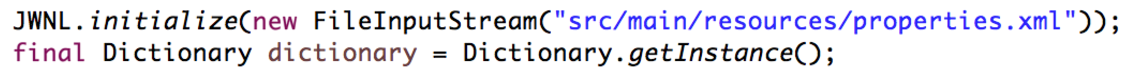
\includegraphics [width=4in,height=4in,keepaspectratio] {jwnl-instantiation.png}      %-- include image file named as "disneychart.png" 
	\caption{Instantiation of the Dictionary}
	\label{fig:jwnl-instantiation}
\end{figure}

Afterwards, a lemma can easily be queried from the dictionary (e.g. travel). For each lemma, there can be one part-of-speech specified among four possible part-of-speech classes: \textit{POS.ADJECTIVE}, \textit{POS.ADVERB}, \textit{POS.NOUN}, and \textit{POS.VERB}. 

The system checks if the lemma is in the dictionary. If the lookup fails, \textit{indexWord} is null as shown in \figref{fig:wn-indexword}.

\begin{figure}[!htb]                %-- use [t] to place figure at top, [b] to place at the bottom, [h] for here
	\centering                    %-- use this to center the figure
	
\includegraphics [width=4in,height=4in,keepaspectratio] {wn-indexword.png}      %-- include image file named as "disneychart.png" 
	\caption{Setting the lemma and part of speech}
	\label{fig:wn-indexword}
\end{figure}

Different senses that the lemma may have are retrieved as shown in Figure \figref{fig:wn-senses}.

\begin{figure}[!htb]                %-- use [t] to place figure at top, [b] to place at the bottom, [h] for here
	\centering                    %-- use this to center the figure
	
\includegraphics [width=4in,height=4in,keepaspectratio] {wn-senses.png}      %-- include image file named as "disneychart.png" 
	\caption{Getting related senses}
	\label{fig:wn-senses}
\end{figure}

For each sense, a short description of the sense called \textit{gloss} is derived as shown in \figref{fig:wn-gloss}. 

\begin{figure}[!htb]                %-- use [t] to place figure at top, [b] to place at the bottom, [h] for here
	\centering                    %-- use this to center the figure
	
\includegraphics [width=4in,height=4in,keepaspectratio] {wn-gloss.png}      %-- include image file named as "disneychart.png" 
	\caption{Getting short description of senses}
	\label{fig:wn-gloss}
\end{figure}

Other more specific lemmas under each sense are also derived as shown in \figref{fig:wn-words}. 

\begin{figure}[!htb]                %-- use [t] to place figure at top, [b] to place at the bottom, [h] for here
	\centering                    %-- use this to center the figure
	
\includegraphics [width=4in,height=4in,keepaspectratio] {wn-words.png}      %-- include image file named as "disneychart.png" 
	\caption{Getting words under specific senses}
	\label{fig:wn-words}
\end{figure}

WordNet returns senses containing related lemmas as shown in \figref{fig:wn-output}.

\begin{figure}[!htb]                %-- use [t] to place figure at top, [b] to place at the bottom, [h] for here
	\centering                    %-- use this to center the figure
	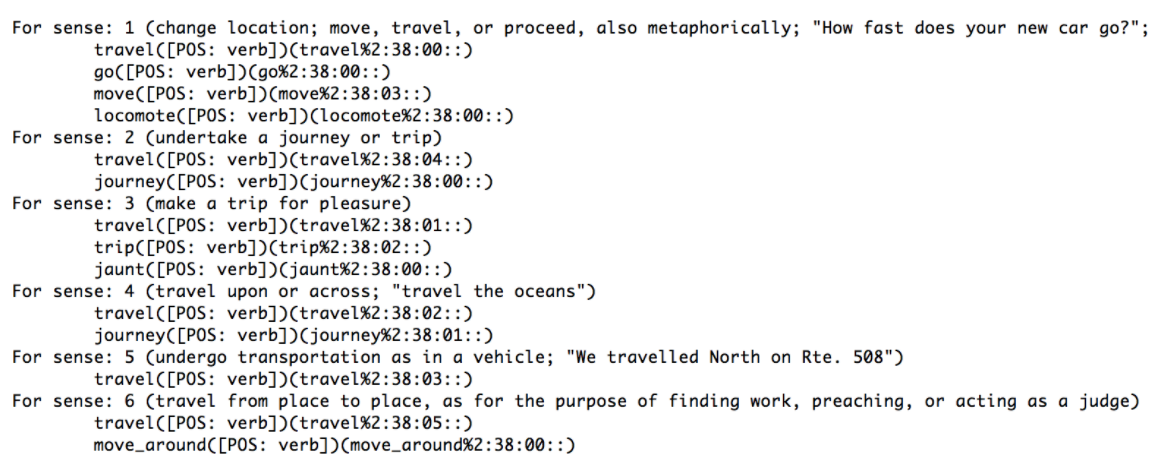
\includegraphics [width=4in,height=4in,keepaspectratio] {wn-output.png}      %-- include image file named as "disneychart.png" 
	\caption{Related senses returned by WordNet}
	\label{fig:wn-output}
\end{figure}

By using the mapping available on WordNet's database, morphosemantically-related words are extracted as shown in \figref{fig:wn-output2}.

\begin{figure}[!htb]                %-- use [t] to place figure at top, [b] to place at the bottom, [h] for here
	\centering                    %-- use this to center the figure
	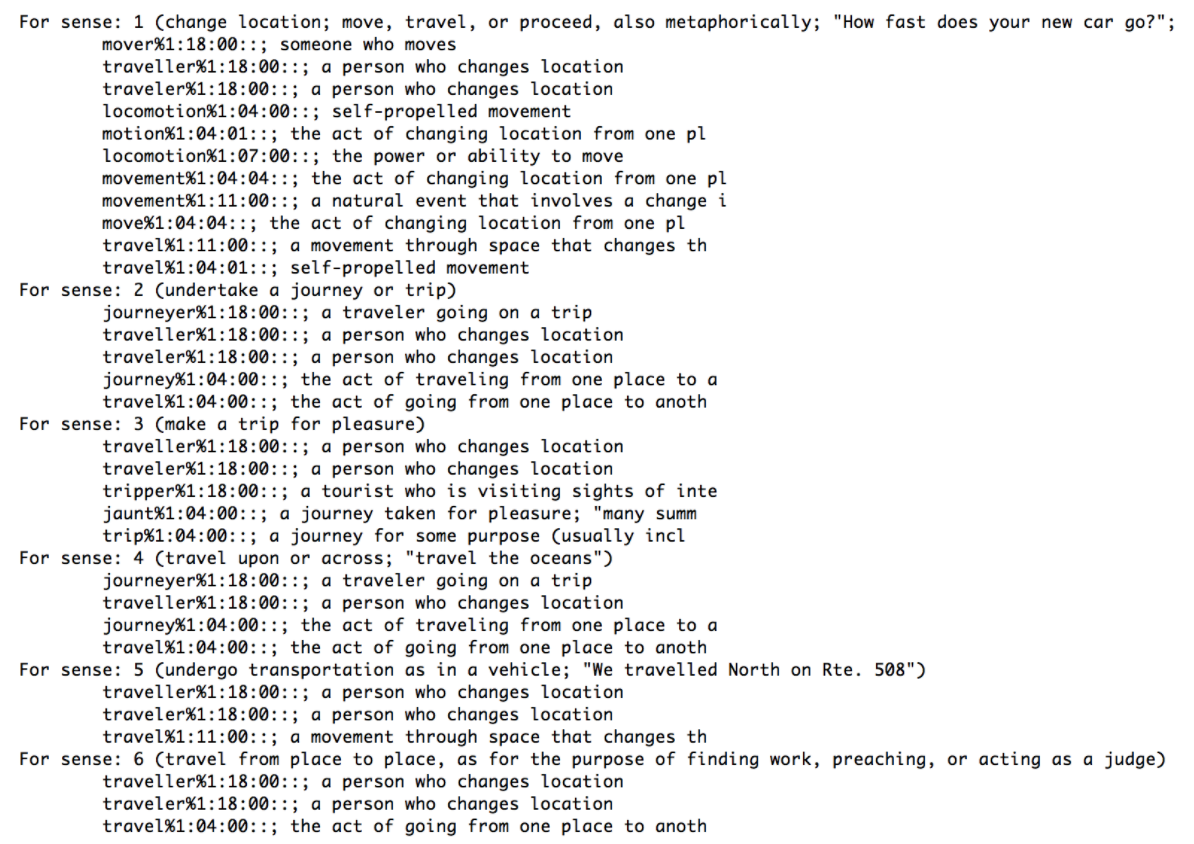
\includegraphics [width=4in,height=4in,keepaspectratio] {wn-output2.png}      %-- include image file named as "disneychart.png" 
	\caption{Morphosemantically related words returned by WordNet}
	\label{fig:wn-output2}
\end{figure}

\subsection{ConceptNet}
ConceptNet is a semantic network containing nodes or concepts which are represented by words or short phrases (e.g. ``ball'', ``toy'') and the semantic relations between them (e.g. ``IsA'', ``PropertyOf'') \footnote{http://conceptnet5.media.mit.edu/}. This contains things that computers should know about the world specifically when understanding text written by human. The relationships labeled between them will help computers in searching information, answering questions and understanding humans. ConceptNet contains everyday basic knowledge, cultural knowledge, and scientific knowledge. ConceptNet also supports language like Chinese and Japanese. 

Previous data from ConceptNet are from a home-grown crowd-sourced project which a website is ran to collect facts from humans who visits the site. The ConceptNet 5.0's knowledge base currently contains 12.5 million edges, representing 8.7 million assertions and connecting 3.9 million concepts into a semantic network of more than 2.78 million nodes which are classified into 23 semantic relations as discussed in ConceptNet5 wiki website \cite{Speer2012}. 

ConceptNet5 \footnote{http://conceptnet5.media.mit.edu/} has a REST API which according to ConceptNet allows the user to: (1) retrieve the data from the nodes and edges, (2) query the edges given a property, and (3) measure and query the semantic distance between two nodes.

%section~~~~~~~~~~~~~~~~~~~~~~~~~~~~~~~~~~~~~~~~~~~~~~~~~~~~~~~~~~~~~~
\section{Evaluation Metrics}
Evaluation metrics are used to evaluate the effectiveness of computer systems and to justify its developments of these systems \cite{PehcevskiPiwowarski2009}. They are necessary to have a formal method of objectively determining the shortcomings of the system in order to be able to improve it. For this research, the three general topics to tackle in the evaluation metrics are [1] the content and quality of the story; [2] the style and appropriateness of writing; and [3] the algorithms under the hood that worked to provide the generated story.

In this research, the primary component to be evaluated is the quality of the resulting life stories, in terms of completeness. When evaluating the writing of a beginner such as a human child, an article by \cite{Hamilton} suggests that the focus should be on the content of the story rather than mechanical errors such as those involving spelling or punctuation. As mentioned in 3.1.1 Elements and Structure of a Story, some elements of a life story may not be present in this generated story due to the age of the person being talked about. However, there is still plenty of content available in Facebook data.

The life story should be composed of three main parts: [1] the introductory part, which introduces the person and presents some interesting facts about him/her; [2] the body part tells stories about the person that had happened in his/her life; and finally, a [3] conclusion part that describes the person's preferences and likes. A life story is deemed complete if these parts are present in the story and can be easily identified by the reader.

The introductory part should contain all the basic information about the user such as the name, birthdate, birthplace, and other profile information that are available. It should correctly follow the structure of the templates described in Appendix \ref{sec:appendixi}, Knowledge Representation, and filled with the correct data. The body part should contain relevant posts relating to one's life events. This requires validating  the algorithms used for post selection and story generation (specifically content determination and sentence aggregation).  Finally, the conclusion should specify five of the user's top preferences, with some other sentences describing how much this person likes those preferences.

In addition, the events specified in the generated story should be traceable from the data extracted from the user. The user should be able to infer that an event in the story came from a specific post that indicates that this event happened. This can be made easier by including time elements in the generated story (e.g. ``last year'', ``two months ago''). The correctness of the content determination would be dependent on the quality and amount of data that can be extracted from the user's Facebook posts.

Another consideration for the evaluation metrics is analyzing the style of writing, as inspired by the works of \cite{Mcgraw2000}. Do the words flow together nicely, for example? For this question, the story should be checked to determine if lexical choices consistently use the correct words, including the discourse markers used to connect the different events and posts to generate coherent stories. Also, is there a sense of organization and focus in the writing of the story? Does it have a strong beginning and a good ending? Are there enough details provided to describe the person? Finally, is the writing free of misspellings, wrong capitalizations, wrong tense use, and wrong use of punctuations?

Lastly, another consideration of the evaluation metrics should be the system architecture itself -- the different algorithms used by the software (described in Chapter 4, particularly in 4.4, Architectural Design). Every process must be validated, in terms of functionality and quality. For example, did the system extract all needed data and store them correctly? Did the text understanding API return the correct entities (as described in Section 3.4.1, Entity Recognition) and did so correctly? Is the knowledge base present and working properly, and was it shown in the generated story that it worked properly and was utilized correctly? Finally, did the text generation process generate a story that meets the primary criteria of the evaluation metrics-- content and style?

Results from evaluation can then be used to improve the quality of the output of this research, which will be described in the next chapter: the system design.

%%%%%%%%%%%%%%%%%%%%%%%%%%%%%%%%%%%%%%%%%%%%%%%%%%%%%%%%%%%%%%%%%%%%%%%%%%%%%%%%%%%%%%%%%%%%%%%%%%%%%%
%
%   Filename    : chapter_4.tex 
%
%   Description : This file will contain your System.
%                 
%%%%%%%%%%%%%%%%%%%%%%%%%%%%%%%%%%%%%%%%%%%%%%%%%%%%%%%%%%%%%%%%%%%%%%%%%%%%%%%%%%%%%%%%%%%%%%%%%%%%%%
\newcommand{\systemname}{FB Stories } 

\chapter\systemname
\label{sec:\systemname}

This chapter discusses the functional requirements and the overall specifications of the software developed as part of this research, called \systemname. It introduces the software, its objectives, scope and limitations, architecture, and features.

%section~~~~~~~~~~~~~~~~~~~~~~~~~~~~~~~~~~~~~~~~~~~~~~~~~~~~~~~~~~~~~~
\section{An Overview}
\systemname is a web-based application where Facebook users can generate their own life stories through the data gathered from their Facebook account, with the use of natural language processing (NLP) and generation (NLG) techniques. 

To use \systemname, the user must log in to their Facebook account to allow access to their data. The data extracted will be classified as either direct knowledge or indirect knowledge. For indirect knowledge, text understanding techniques will be applied. 

The software then proceeds to the text generation module, where it determines which elements of the extracted data are appropriate and can be used in generating the life story, and constructs corresponding story text from these data. Once the life story text has been generated, the user is given the option to save the story into a text file.

The completed life story contains three parts. The first part contains basic information or facts about the user. The second part contains data extracted from the Facebook posts that were classified and stored into the indirect knowledge base. The third part contains the list of preferences of the user inferred from the available list of page likes, as well as some recent events that this person has attended.

%section~~~~~~~~~~~~~~~~~~~~~~~~~~~~~~~~~~~~~~~~~~~~~~~~~~~~~~~~~~~~~~
\section{Software Objectives}
This section presents the general and specific objectives of \systemname.

\subsection{General Objective}
To generate a story that takes into account the Facebook posts of a user by using natural language processing techniques.

\subsection{Specific Objectives}
\begin{enumerate}
\item To extract needed data from Facebook;
\item To use data processing techniques to analyze the input; 
\item To classify each post according to its type;
\item To use text generation techniques to generate a story;
\item To allow users to save the generated stories into a text file.
\end{enumerate}

%section~~~~~~~~~~~~~~~~~~~~~~~~~~~~~~~~~~~~~~~~~~~~~~~~~~~~~~~~~~~~~~
\section{Scope and Limitations of the Software}

\subsection{Data Extraction}
In retrieving data from a user's Facebook account, asking for user's permission is necessary. A successful login to the user's Facebook account means that the user permits the system to make use of their data. These permissions will be readily set out for the user to approved, and once set, selected options cannot be altered. If the user does not allow the software to access his/her profile with the given permissions, only those public information and public posts of the user are extracted. 

\systemname does not extract data from Messenger, as well as information about the user's interactions (such as who Liked the user's posts).

\subsection{Data Processing}
Data processing techniques are only applicable to Facebook posts. The system does not perform any verification on the correctness of the user's  data.

Hashtags, hyperlinks, emoticons, laughter, and foreign characters are removed from posts before undergoing text understanding, in order to lessen misclassifications. For posts with mixed languages, abbreviations and incomplete sentences, the interpretation of these are limited by what the API can offer \figref{fig:MixedLanguage}. The syntax analysis returned by the tool is not checked for the correctness of its output. In \figref{fig:MixedLanguage}, ``kain” is a Filipino word which means ``eat”, thus it should be a verb not a noun. 

\begin{figure}[!htb]                %-- use [t] to place figure at top, [b] to place at the bottom, [h] for here
   \centering                    %-- use this to center the figure
   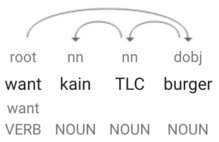
\includegraphics [width=2.5in,height=2.5in,keepaspectratio] {MixedLanguage.png}      %-- include image file named as "disneychart.png" 
   \caption{Sample Incomplete Text with Mixed Languages and Abbreviation.}
    \label{fig:MixedLanguage}
\end{figure}

\subsection{Post Classification}
Posts extracted from Facebook cannot be used directly in generating story text, since users tend to post snippets of incomplete, context-based data. Other posts have no explicit verbs used to describe the event. Thus, the posts must be individually processed to extract the necessary information comprising an event.

Although Facebook has a feature called \textit{Predefined Activities} to enable users to easily  classify their individual posts according to the content, there are currently no tools that can support the extraction of relevant elements from posts that uses this feature. Thus, a post classification algorithm is needed to classify each Facebook post as either \textit{celebrating} post, \textit{travelling} post, \textit{drinking} post, \textit{eating} post or \textit{no event} post. These four types of posts are chosen to be used in this research since majority of Facebook posts gathered and analyzed fall under them. Other types of posts such as \textit{reading}, \textit{listening}, \textit{watching}, among others may be present in the extracted Facebook posts, but will be ignored and will be tagged as \textit{no event} posts for this research.

\subsection{Text Generation}
Text generation has three components. One component is responsible for generating the introductory part of the story text, the second component is responsible for generating the body and the last component is responsible for generating the conclusion.

The introduction contains basic information directly extracted from the user's profile without going through further processing. The body part of the life story contains events: information which underwent processing and post classification. The conclusion part of the life story contains the likes and preferences of the user, as well as recent Facebook Events attended. 

\subsection{Save to Text File}
The user might want to cherish and read previously generated life stories in the future, making it important to have a method to save stories. Text files are only generated based on the user's instructions. Other file types than \textit{.txt} are not supported. After successfully saving the generated story into a text file, the user is solely responsible for the safekeeping and/or dissemination of the file.

For purposes of validating the output of FB Stories and for future research, a copy of the generated life story is also stored as part of the output of this research. The user is properly informed of this. Anonymizing the data for future use is provided as an option for confidentiality

\clearpage
%section~~~~~~~~~~~~~~~~~~~~~~~~~~~~~~~~~~~~~~~~~~~~~~~~~~~~~~~~~~~~~~
\section{Architectural Design}
\figref{fig:AD} is a representation of the architecture design of \systemname. It is divided into three big parts: initialization, text understanding, and text generation.

A more detailed discussion of the different modules is written in Chapter 5 for both the initial version of the system as well as the latest version as of the time of writing.

\begin{figure}[!htb]                %-- use [t] to place figure at top, [b] to place at the bottom, [h] for here
   \centering                    %-- use this to center the figure
   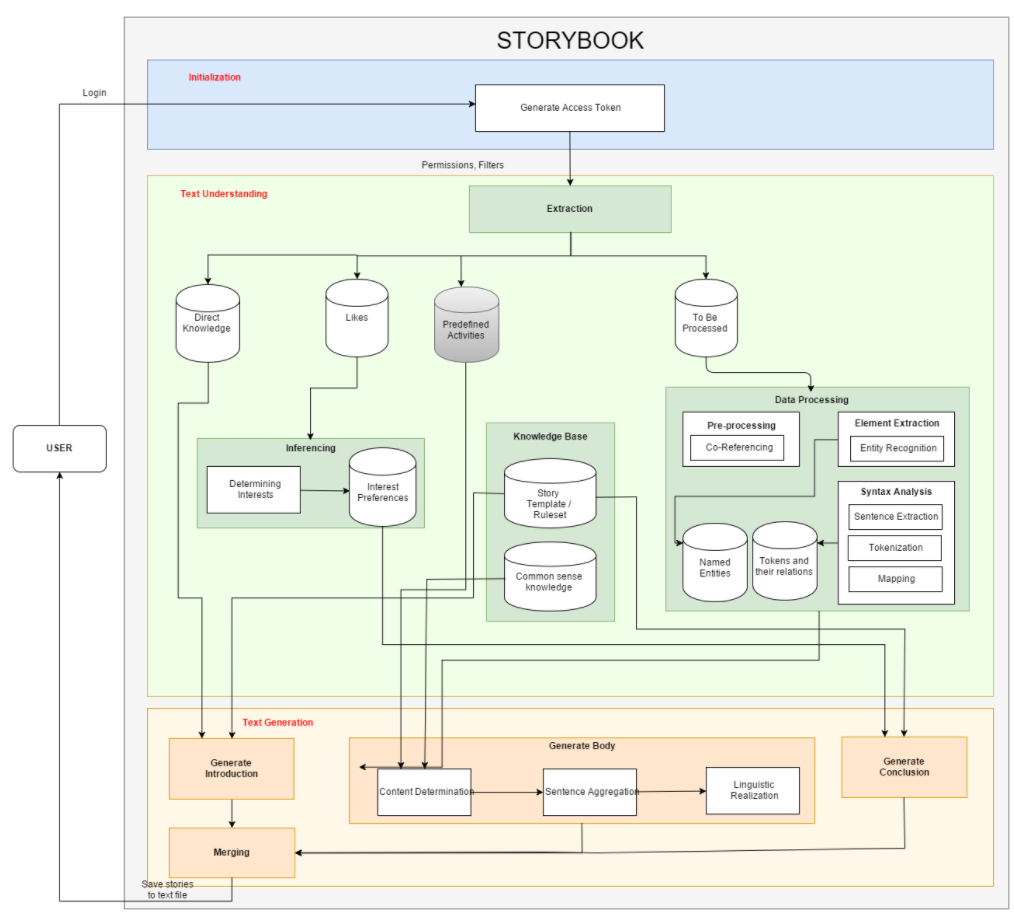
\includegraphics [width=\textwidth] {AD.png}      %-- include image file named as "disneychart.png" 
   \caption{Architecture Design of \systemname}
    \label{fig:AD}
\end{figure}

\subsection{Initialization}
Before the system can extract the user's data, it needs the user's permission, which the user grants by logging into Facebook and specifying that they agree with the data extraction to be done by FB Stories. After the user goes through each of the permissions and accepts it, Facebook generates an access token, which controls which data can be extracted by the data extraction tool.

The data extracted can be classified into one of three types:
\begin{itemize}
	\item \textit{Direct knowledge}. These are derived from the user's \textit{About Me} section, and are used for generating the introductory part of the life story.
	\item \textit{Data to be processed}. These are taken from the user's posts on their Timeline, and will be processed later on for use in generating the body.
	\item  \textit{User's list of Liked pages and Facebook Events}. These are derived from the user's account (Facebook keeps track of the user's list of Liked pages and Facebook Events attended). These will be used as part of the conclusion.
\end{itemize}

\subsection{Text Understanding}
For those data from which knowledge cannot be easily inferred, a more specific procedure of text understanding algorithms is applied. Data preprocessing processes the input in order to deal with issues present in user-generated data, such as stray characters or the presence of laughter. 

After preprocessing these data, they are then subjected to NLP processes which enable the system to figure out the relevant parts of these data to use in generating the story later on, such as who did what, what is being done, and to whom or to what. These data are then classified (with the help of the knowledge base) in order to figure out how they'll be organized in the final generated story. 

\subsection{Text Generation}
The text generation module is responsible for generating the appropriate story segments that make up the entire life story generated by FB Stories. There are three components: the \textit{GenIntro}, \textit{GenBody}, and \textit{GenConclusion}.

GenIntro uses data determined to be ``facts'' or direct knowledge. It involves checking the knowledge base for the appropriate template to be used based on the available facts in the \textit{Direct Knowledge}, \textit{Educational Background}, \textit{Work}, and \textit{Family} table. GenIntro would also involve filling the template with the correct data. The generated text will become the introductory paragraph of the life story.

GenBody, on the other hand, is applied to generate the body of the life story from the data processed in the Data Processing module. The body paragraph(s) will be narrating one or more events about a person's life. These events will be taken from data that users have written and posted on their own Timeline. For these data, text generation is more complex. It will undergo three sub-modules, which are all detailed in Section 3.5.1, Text Generation.

GenConclusion will be used to generate the conclusion part of the story text, which will contain the user's likes and interested events. The exact process of determining the user's likes is explained in the Inferencing Section, 4.4.4. Similar to the approach in GenIntro, GenConclusion would check the available templates defined in the Template table and use the data stored in the \textit{Likes} and \textit{Events} table.

The generated texts from the three text generation modules are then merged, and presented to the user as the complete life story. The user will now have the option to save or discard their life story. If the user wishes to save their life stories, a text file will be created and the user chooses where to save this file. But if the user wishes to discard this, then they simply close the software.

%section~~~~~~~~~~~~~~~~~~~~~~~~~~~~~~~~~~~~~~~~~~~~~~~~~~~~~~~~~~~~~~
\section{Software Functions}
FB Stories provides a simple environment that allows users to easily use it to create a life story from their Facebook posts and save these stories for future use. Below are the software functions used in FB Stories.

\subsection{Login Window}
Upon starting the application, FB Stories' main screen was displayed as shown in \figref{fig:MainScreen}, it contains the login or logout button, name of the logged in user, Try Me button, Show Output button, and Help button.

\begin{figure}[!htb]                %-- use [t] to place figure at top, [b] to place at the bottom, [h] for here
   \centering                    %-- use this to center the figure
   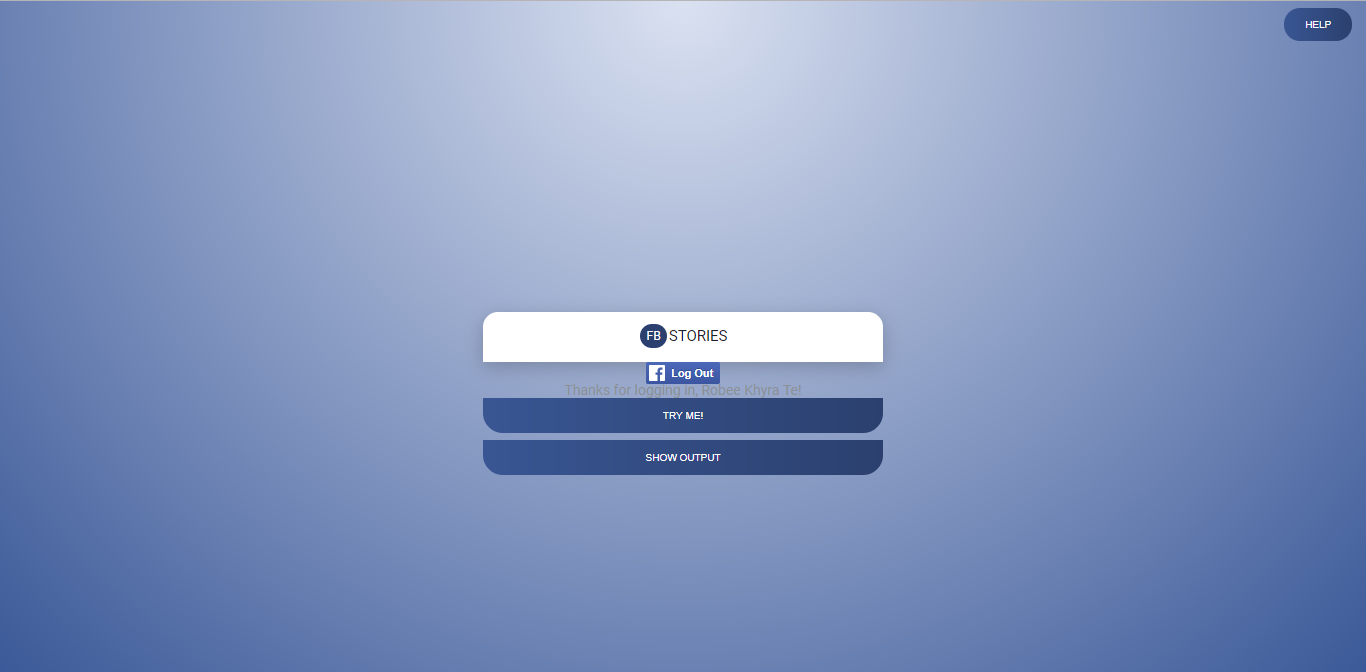
\includegraphics [width=3in,height=2in,keepaspectratio] {MainScreen.png}      %-- include image file named as "disneychart.png" 
   \caption{FB Stories' Main Screen.}
    \label{fig:MainScreen}

\subsection{Help Window}
In order to ensure the user about the process, a help window as shown in \figref{fig:HelpWindow}, is there to provide the necessary information about it. 

\begin{figure}[!htb]                %-- use [t] to place figure at top, [b] to place at the bottom, [h] for here
   \centering                    %-- use this to center the figure
   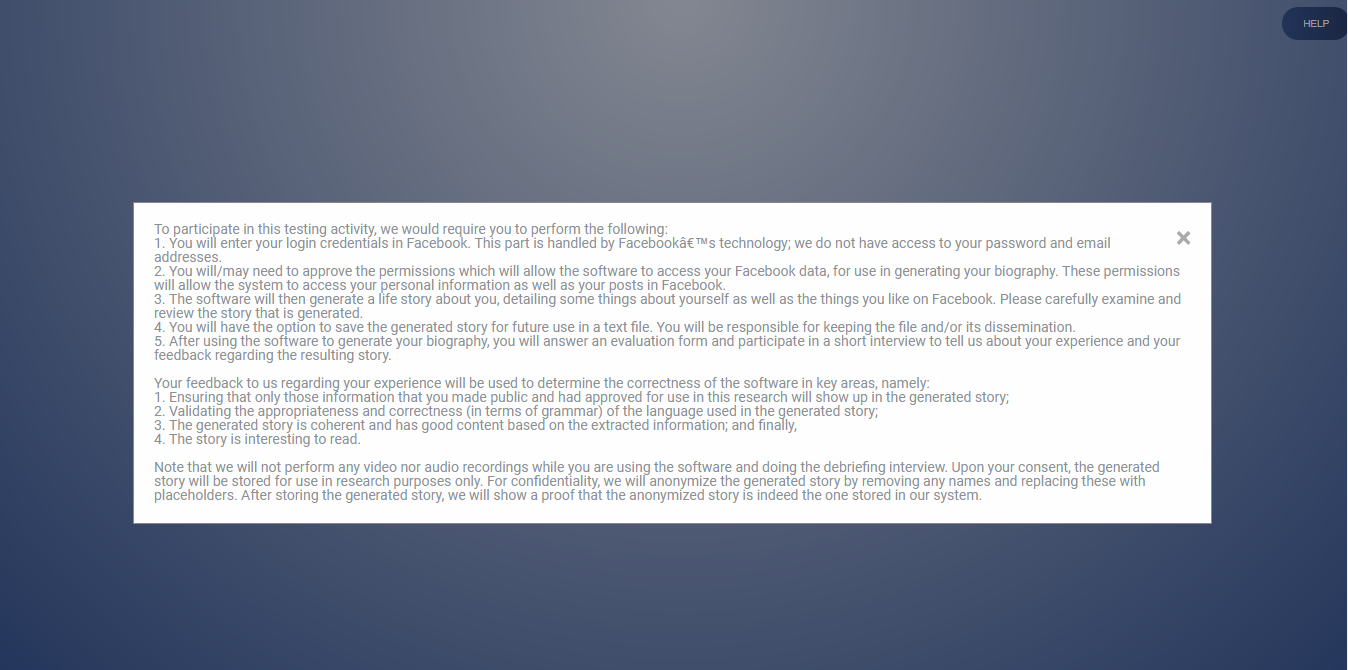
\includegraphics [width=3in,height=2in,keepaspectratio] {HelpScreen.png}      %-- include image file named as "disneychart.png" 
   \caption{Help Window.}
    \label{fig:HelpWindow}

\subsection{Login Window}
In using the application, the user would have to Login to Facebook for the software to access the data stored in his/her account. A Facebook login button would prompt the user to login as shown in \figref{fig:Login}. Once the button is clicked, a Login Window, which can be seen in \figref{fig:Login2}, would pop up informing the user that he/she is logging in his/her Facebook account with the app, StoryBook. Login information such as email address, phone number or user id along with the corresponding password are both needed to successfully login. 

Logging in to the app also grants the permissions set by the app which then automatically updates the access token stored in cookies. 

\begin{figure}[!htb]                %-- use [t] to place figure at top, [b] to place at the bottom, [h] for here
   \centering                    %-- use this to center the figure
   
\includegraphics [width=3in,height=2in,keepaspectratio] {login1.png}      %-- include image file named as "disneychart.png" 
   \caption{Facebook Login Button.}
    \label{fig:Login}
\end{figure}

\begin{figure}[!htb]                %-- use [t] to place figure at top, [b] to place at the bottom, [h] for here
   \centering                    %-- use this to center the figure
   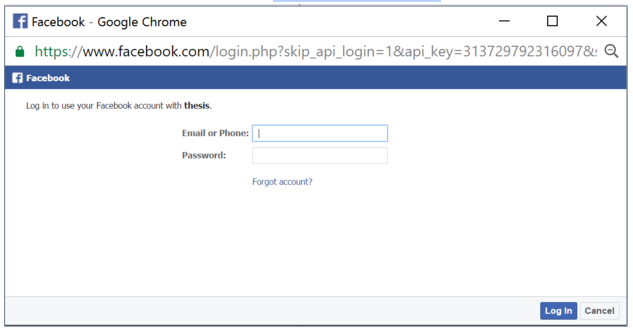
\includegraphics [width=\textwidth] {login2.png}      %-- include image file named as "disneychart.png" 
   \caption{Pop-up Login Window.}
    \label{fig:Login2}
\end{figure}

\subsection{Permission Window}
Logging in to Facebook automatically stores a default access token in cookies. If the user is already logged-in on Facebook and the \systemname automatically obtains the user's access token, then it would check permissions in the access token and prompts the user of the missing permissions it needs to acquire. \figref{fig:Permission} displays the permission window that asks the user to grant the permissions needed by the software.

\begin{figure}[!htb]                %-- use [t] to place figure at top, [b] to place at the bottom, [h] for here
   \centering                    %-- use this to center the figure
   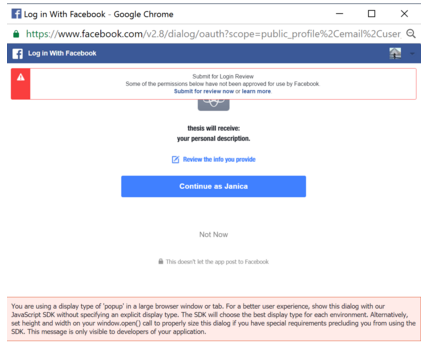
\includegraphics [width=\textwidth] {permission.png}      %-- include image file named as "disneychart.png" 
   \caption{Permission Window.}
    \label{fig:Permission}
\end{figure}

\subsection{Generated Story Output Window}
The Generated Story Output Window, \figref{fig:Output}, is basically a window that displays the generated story after FB Stories has analyzed and processed the gathered data from the user's Facebook account. The user would be given an option to save the generated story to a text file through the ``Save to Text File" button.

\begin{figure}[!htb]                %-- use [t] to place figure at top, [b] to place at the bottom, [h] for here
   \centering                    %-- use this to center the figure
   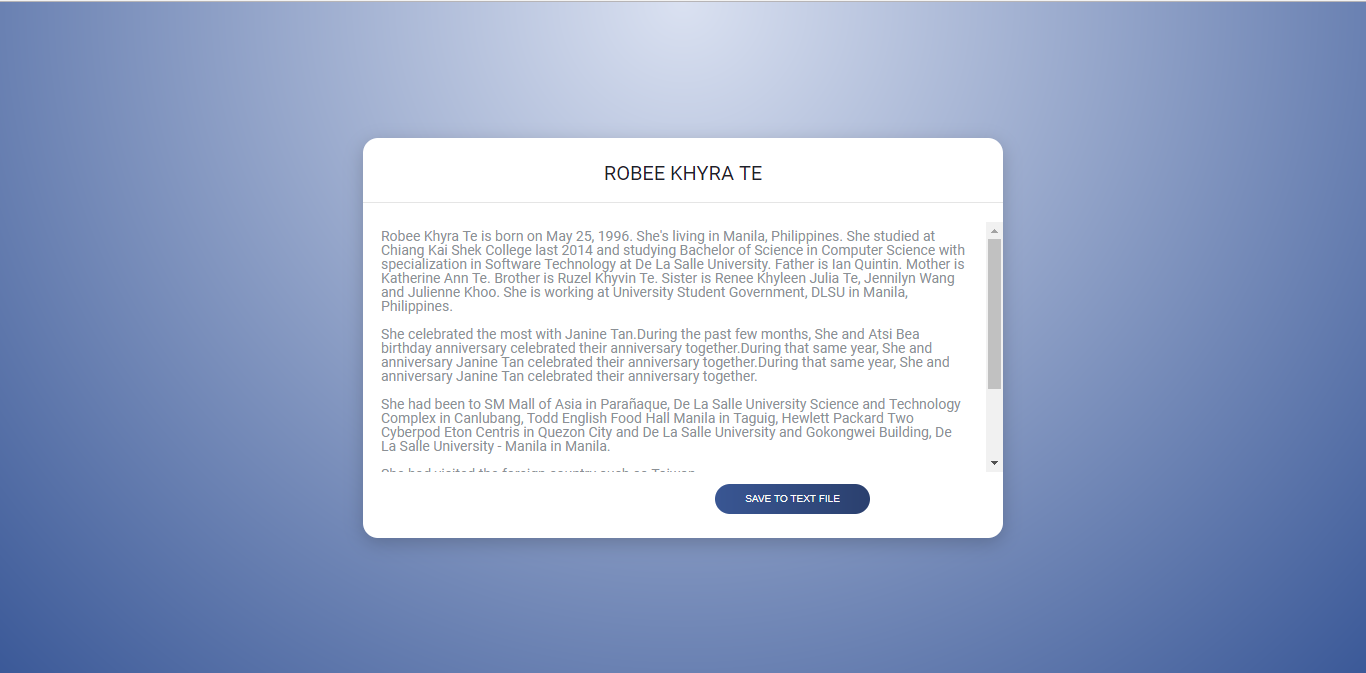
\includegraphics [width=\textwidth] {GeneratedStoryOutputWindow.png}      %-- include image file named as "disneychart.png" 
   \caption{Generated Story Output Window.}
    \label{fig:Output}
\end{figure}
\clearpage

\subsection{Sample Saved Text File}
After the user had successfully saved his/her own life story as a text file as shown in \figref{fig:SampleTextFile}, he/she can view it in any text editor application.

\begin{figure}[!htb]                %-- use [t] to place figure at top, [b] to place at the bottom, [h] for here
   \centering                    %-- use this to center the figure
   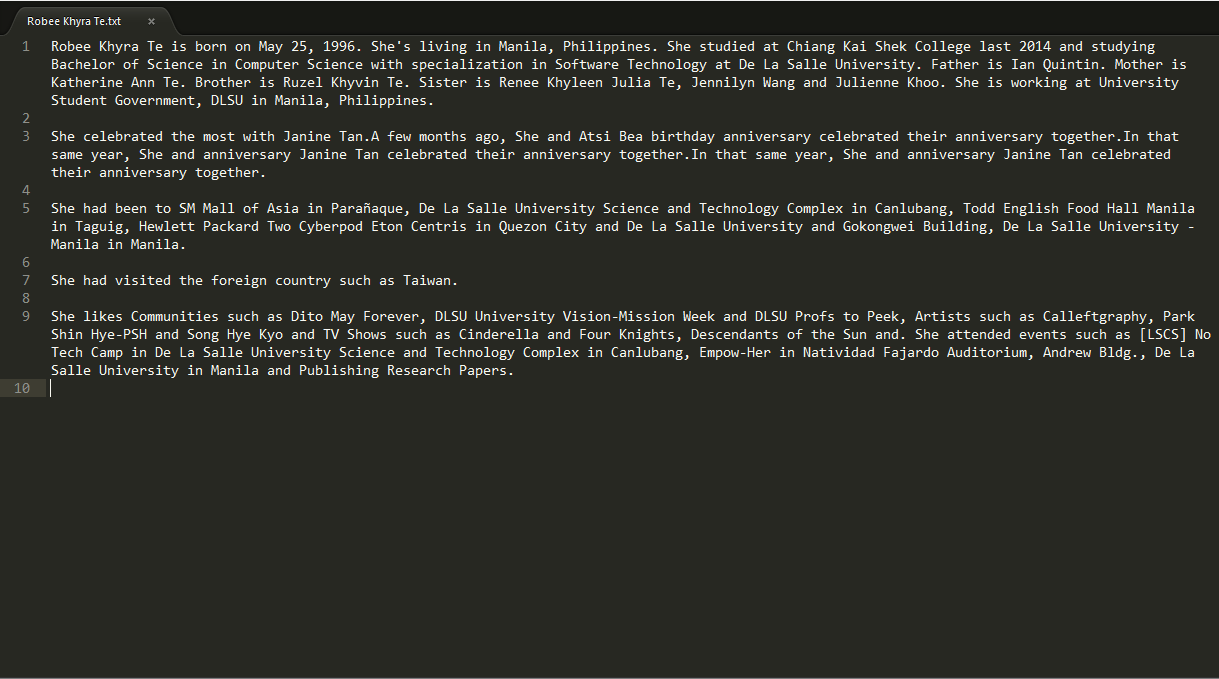
\includegraphics [width=\textwidth] {SampleTextFile.png}      %-- include image file named as "disneychart.png" 
   \caption{Sample Text File.}
    \label{fig:SampleTextFile}
\end{figure}


\section{Physical Enviroment and Resources}
This section details the minimum and recommended software requirements for software implementation.

\systemname requires the following resources for development:
\begin{itemize}
\item Eclipse IDE
\item MySQL Server and Workbench
\item Java Development Kit (JDK)
\item Apache Tomcat 8.0
\end{itemize}

These are the minimum software requirements for \systemname to run properly:
\begin{itemize}
\item \textbf{OS}: Windows 7 / 8.1 / 10
\item \textbf{Memory}: 1 GB RAM
\item \textbf{Storage}: At most 1 GB of free hard disk space
\item \textbf{Internet connection}: Broadband, at least 1Mb/s bandwidth
\item \textbf{Others}: Java Runtime Environment (JRE), MySQL Server, Apache Tomcat 8.0, Any Web Browser
\end{itemize}

\subsection{Tools}
The following tools will be used for the development and runtime of the \systemname.

\subsubsection{Facebook Login API}
The Facebook Login API enables the use of the Facebook user's identity in order to craft interesting stories about them. It enables the application to extract data from Facebook to be processed and used to generate stories. Features of Facebook Login, such as access tokens and permissions, make it safe and secure for people and apps to use, but there are some security steps which this software will need to implement. This will be tackled in Chapter 5, Design and Implementation.

\subsubsection{Graph API}
The use of Graph API enables the software to extract posts and data from a specific Facebook account. It supports developers by supplying services such as providing snippets of codes for easier integration with JSON requests and responses.

\subsubsection{Stanford CoreNLP}
Stanford CoreNLP will be used in the text understanding module, as it provides the needed component, syntax analysis. 

\subsubsection{WordNet}
WordNet will be used to supply the data that is needed for the reference table which contains keywords such as related verbs and nouns. The reference table will then be used in the classification of Facebook post which does not contain a verb.

\subsubsection{ConceptNet}
ConceptNet is a semantic network containing concepts with Open Mind Common Sense as its main source of knowledge, along with other sources such as Wikipedia, WordNet, and DBPedia. This knowledge will be used to supply keywords for the reference table to be used in the post classification module. This will gather related verbs and noun for the categories \textit{Celebrating}, \textit{Travelling}, \textit{Eating}, and \textit{Drinking}.

\subsubsection{SimpleNLG}
SimpleNLG will be used in generating grammatically correct English sentences. SimpleNLG will also automate some of the tasks an NLG system needs to perform like checking the orthography, morphology and simple grammar of the sentences.

\chapter{Design and Implementation}
\label{sec:designandimplementation} 

This chapter presents the design and implementation of StoryBook. It first discusses the authors' journey in dealing with the data in Facebook and the issues inherent in its characteristics. This is followed by the discussion on the event classification algorithm of the system, its issues, initial shortcomings, and improvements. It ends with a discussion of the natural language generation module, which has three submodules: the GenIntro, GenBody, and GenConclusion. The issues encountered during implementation and the solutions applied to address each issue are presented.

%section~~~~~~~~~~~~~~~~~~~~~~~~~~~~~~~~~~~~~~~~~~~~~~~~~~~~~~~~~~~~~~
\section{System Design}
\figref{fig:IAD} shows the system architecture of \systemname.

\begin{figure}[!htb]                %-- use [t] to place figure at top, [b] to place at the bottom, [h] for here
	\centering                    %-- use this to center the figure
	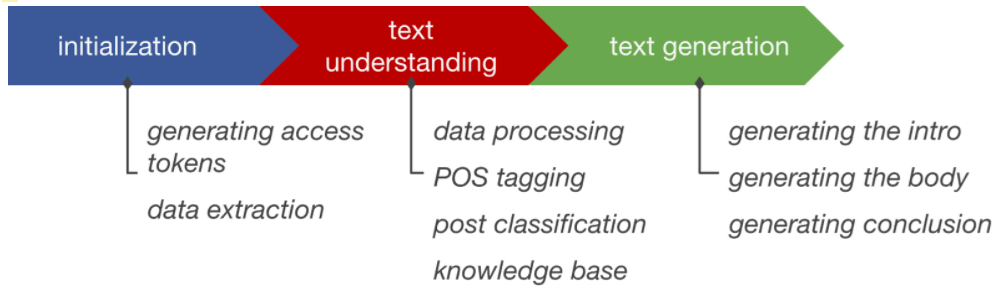
\includegraphics [width=\textwidth] {IAD.png}      %-- include image file named as "disneychart.png" 
	\caption{System Architecture of \systemname}
	\label{fig:IAD}
\end{figure}

\subsection{Initialization}
\textit{Part of: Startup} \newline \newline
The user, via the use of the Facebook Login API \cite{FacebookLogin}, must give his/her login credentials to allow their Facebook data to be extracted for use. After the user goes through each of the permissions and allows them, Facebook generates an access token, which is then used by Graph API to determine which data can be extracted from the Facebook account of the user.

\subsection{Data Extraction}
\textit{Part of: Text Understanding} \newline \newline
This uses Graph API. Three types of data need to be extracted and partitioned into: [1] personal info that can be used as is, such as the user's birthday and list of family members; [2] data which have to be processed such as posts; and [3] the user's list of preferences and events attended. 

The partitioned data will be stored in seven separate tables: direct\_knowledge, educational\_bg, work, family, to\_be\_processed, likes and events, as shown in \figref{fig:ExtractedDataDB}. 

\begin{figure}[!htb]                %-- use [t] to place figure at top, [b] to place at the bottom, [h] for here
	\centering                    %-- use this to center the figure
	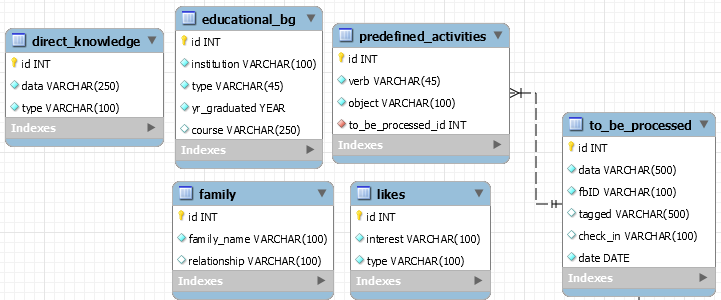
\includegraphics [width=\textwidth] {ExtractedDataDB2.png}      %-- include image file named as "disneychart.png" 
	\caption{Database Design for Storing Extracted Data.}
	\label{fig:ExtractedDataDB}
\end{figure}

Direct knowledge can be extracted from Facebook's About Me section, which contains the personal information of the user. The extracted data also known as the direct knowledge or facts about the user are stored in the \textit{Direct Knowledge Table} (Table \ref{tab:DirectKnowledge}), which contains the following fields:
\begin{itemize}
	\item id - unique value that identifies each fact
	\item data - the direct knowledge data extracted from his/her Facebook account
	\item type - the type of knowledge that describes the data
\end{itemize}
See Appendix \ref{sec:appendixi} for the complete list of types available and a description of each.

Given the sample \textit{About Me} section of a user in Facebook (\figref{fig:AboutMe}), some of the data are shown in Table \ref{tab:DirectKnowledge}:

\clearpage
\begin{figure}[!htb]                %-- use [t] to place figure at top, [b] to place at the bottom, [h] for here
	\centering                    %-- use this to center the figure
	\includegraphics [width=6in,height=4in,keepaspectratio] {AboutMe.png}      %-- include image file named as "disneychart.png" 
	\caption{Sample About Me Section in Facebook}
	\label{fig:AboutMe}
\end{figure}

\begin{table}[ph!]   %t means place on top, replace with b if you want to place at the bottom
	\centering
	\caption{Sample data in the direct\_knowledge table.} \vspace{0.25em}
	\begin{tabular}{|p{1.5cm}|p{2in}|p{1.5in}|} \hline
		\textbf{id} & \textbf{data} & \textbf{type} \\ \hline
		1 & Robee Khyra Te & name \\ \hline
		2 & NULL & middle\_name \\ \hline
		3 & Te & last\_name \\ \hline
		4 & 1996-05-25 & birth\_date \\ \hline
		5 & Manila, Philippines & location \\ \hline
	\end{tabular}
	\label{tab:DirectKnowledge}
\end{table}

The educational background of the user can also be extracted from Facebook's \textit{About Me} section. These are then stored in the \textit{Educational Background Table} (Table \ref{tab:EducationalBG}), which contains the following fields:
\begin{itemize}
	\item id - unique value that identifies each educational level
	\item institution - the name of the institution
	\item type - the type of educational level
	\item year\_graduated - year graduated or ended in the institution
	\item course - course taken in the said institution
	\item fbID - unique id generated by Facebook for each institution
\end{itemize}
See Appendix \ref{sec:appendixi} for the complete list of types available and description of each.

\begin{table}[ph!]   %t means place on top, replace with b if you want to place at the bottom
	\centering
	\caption{Sample data in the educational_bg table.} \vspace{0.25em}
	\begin{tabular}{|p{.5cm}|p{1in}|p{1.5cm}|p{2cm}|p{2.5cm}|p{2cm}|} \hline
		\textbf{id} & \textbf{institution} & \textbf{type} & \textbf{year\_ \newline graduated} & \textbf{course} & \textbf{fbID} \\ \hline
		1 & De La Salle University & College & null & Bachelor of Science in Computer Science with specialization in Software Technology &  \\ \hline
		2 & Chiang Kai Shek College & High School & 2013 & null & \\ \hline
	\end{tabular}
	\label{tab:EducationalBG}
\end{table}

Current or previous work of the user can also be extracted from Facebook's About Me section. These are then stored in the \textit{Work Table} (Table \ref{tab:work}), which contains the following fields:
\begin{itemize}
	\item id - unique value that identifies each work
	\item institution - the name of the institution
	\item date\_started - year started working in the institution
	\item date\_ended - year ended working in the institution
	\item location - location of the said institution
	\item fbID - unique id generated by Facebook for each work institution
\end{itemize}

\begin{table}[ph!]  
	\centering
	\caption{Sample data in the work table.} \vspace{0.25em}
	\begin{tabular}{|p{.5cm}|p{1.5in}|p{2cm}|p{2cm}|p{2cm}|p{2.5cm}|} \hline
		\textbf{id} & \textbf{institution} & \textbf{date\_ \newline started} & \textbf{date\_\newline ended} & \textbf{location} & \textbf{fbID} \\ \hline
		1 & University Student Government, DLSU & 2013-09-01 & 2014-04-30 & Manila, Philippines &  
		3459628907221
		\\ \hline
	\end{tabular}
	\label{tab:work}
\end{table}

Family members of the user can also be extracted from Facebook's \textit{About Me} section. These are then stored in the \textit{Family Table} (Table \ref{tab:Family}), which contains the following fields:
\begin{itemize}
	\item id - unique value that identifies each family member
	\item family\_name - name of the family member
	\item relationship - relationship with the user
	\item fbID - unique id generated by Facebook for each family member
\end{itemize}
See Appendix \ref{sec:appendixi} for the complete list of available relationships.

\begin{table}[ph!]   %t means place on top, replace with b if you want to place at the bottom
	\centering
	\caption{Sample data in the family table.} \vspace{0.25em}
	\begin{tabular}{|p{1.5cm}|p{2in}|p{1.5in}|} \hline
		\textbf{id} & \textbf{family\_name} & \textbf{relationship} & \textbf{fbID} \\ \hline
		1 & Jennilyn Wang & sister & \\ \hline
		2 & Renee Te & sister & \\ \hline
	\end{tabular}
	\label{tab:Family}
\end{table}

Data taken from the user's posts, on the other hand, requires further processing.

The assumptions for these posts are:
\begin{enumerate} [label=\alph*.]
	\item They all contain a text portion;
	\item The created time of the original post (in case there were no edits made) is assumed to be the time the event happened;
	\item If there were edits made, the edited time would be used and considered to determine the time sequence of the posts;
	\item The people tagged are used to know that those people are with the user at the time of the event; and
	\item All content provided are correct.
\end{enumerate}

\clearpage
\begin{figure}[!htb]                %-- use [t] to place figure at top, [b] to place at the bottom, [h] for here
	\centering                    %-- use this to center the figure
	\includegraphics [width=5in,height=4in,keepaspectratio] {SamplePost.png}      %-- include image file named as "disneychart.png" 
	\caption{Sample Post in Facebook}
	\label{fig:SamplePost}
\end{figure}

The \textit{To Be Processed Table} (Table \ref{tab:ToBeProcessed}) is used to store the description or caption in the user's status and posts, including other relevant information regarding the posts. The following are the attributes of the \textit{To Be Processed} table:
\begin{itemize}
	\item id - unique value that identifies each post
	\item data - the description/caption extracted from his/her Facebook account
	\item fbID - unique id generated by Facebook for each post
	\item tagged - comma-separated values representing the friends the user is with for each post
	\item place - the place where the event happened
	\item city - the city where the event happened
	\item country - the country where the event happened
	\item year - the year when the post was created
	\item month - the month when the post was created
	\item day - the day when the post was created
\end{itemize}

\begin{table}[ph!]   %t means place on top, replace with b if you want to place at the bottom
	\centering
	\caption{Sample data in the to\_be\_processed table.} \vspace{0.25em}
	\begin{tabular}{|p{1cm}|p{1in}|p{1in}|p{1in}|p{2cm}|p{1.5cm}|} \hline
		\textbf{id} & \textbf{data} & \textbf{fbID} & \textbf{tagged} & \textbf{check\_in} & \textbf{date} \\ \hline
		1 & writing our thesis paper document & 102024790 \newline 48375248 & Janica Mae Lam, Camille Saavedra, Alds Hade & Gokongwei Building, De La Salle University - Manila & 2016-11-22 \\ \hline
	\end{tabular}
	\label{tab:ToBeProcessed}
\end{table}

Given the sample list of user's liked pages section in Facebook (\figref{fig:LikedPage}), the liked data that are stored in the database is shown in Table \ref{tab:Likes}.

\begin{figure}[!htb]                %-- use [t] to place figure at top, [b] to place at the bottom, [h] for here
	\centering                    %-- use this to center the figure
	\includegraphics [width=5in,height=4in,keepaspectratio] {LikedPage.png}      %-- include image file named as "disneychart.png" 
	\caption{Sample Interest Preference in Facebook}
	\label{fig:LikedPage}
\end{figure}

The \textit{Likes Table} (Table \ref{tab:Likes}) contains the interest preferences of a particular user in Facebook. This also specifies what time of interest it is.
\begin{itemize}
	\item id - unique value that identifies each interest
	\item interest - the specific interest liked by the user in his/her Facebook account
	\item type - the type of interest that describes the interest
	\item fbID - unique id generated by Facebook for ech page
\end{itemize}
See Appendix \ref{sec:appendixi} for the complete list of available types.

\begin{table}[ph!]   %t means place on top, replace with b if you want to place at the bottom
	\centering
	\caption{Sample data in the likes table.} \vspace{0.25em}
	\begin{tabular}{|p{1.5cm}|p{2in}|p{1.5in}|} \hline
		\textbf{id} & \textbf{data} & \textbf{type} \\ \hline
		1 & Radio Disney & 121 (Radio Station) \\ \hline
		2 & Bridgit Mendler & 93 (Musician/Band) \\ \hline
		3 & Charlie Puth & 93 (Musician/Band) \\ \hline
		4 & Pitch Perfect & 91 (Movie) \\ \hline
		5 & MTV Asia & 147 (TV Network) \\ \hline
		6 & [V] Hits & 146 (TV Channel) \\ \hline
		7 & The Flash & 149 (TV Show) \\ \hline
		8 & Nickelodeon & 147 (TV Network) \\ \hline
	\end{tabular}
	\label{tab:Likes}
\end{table}

Given the sample list of user's going and interested events in Facebook \figref{fig:events}, the events data that are stored in the database is shown in Table \ref{tab:events1}.

The \textit{Events} table (Table \ref{tab:events1}) contains all the going and interested events of a particular user in Facebook. It contains the following fields:
\begin{itemize}
	\item id - unique value that identifies each interest
	\item name - the specific interest liked by the user in his/her Facebook account
	\item rsvp\_status - the type of interest that describes the interest 
	\item place - the place where the event took place
	\item city- the city where the event took place
	\item country - the country where the event took place
	\item fbID - unique id generated by Facebook for each event
\end{itemize}
See Appendix I for the complete list of types available.
\clearpage

\subsection{Inferencing}
\textit{Part of: Text Understanding} \newline \newline
Some user interests have to be inferred, to answer questions such as, ``how does one determine if one likes music?” This particular question can be answered by looking at the list of a person's liked pages.

Facebook has six (6) general categories for Pages, and around 100 specific categories. For this study, the top five categories with the most liked pages by the user are written down in the story. Narrowing down the categories to the top five allows the life story to focus on the things that the user likes the most.

For instance, if the user likes 87 pages of the category ``Musician/Band” and it falls under the top five categories of pages she has liked, it can be inferred that she likes music. The top five categories are later used in the conclusion. 2-3 sample pages under each category are used in the to provide support.

\subsection{Data Processing}
\textit{Part of: Text Understanding} \newline \newline
This process utilizes Stanford CoreNLP. For those data from which knowledge cannot be easily inferred, a more specific procedure of text understanding algorithms is applied. Data preprocessing processes the input and stores them in an abstract representation for use by other modules of \systemname. Hashtags, hyperlinks, emoticons, laughter, and foreign characters are removed from posts before undergoing text understanding, in order to lessen misclassifications.

After the text has been preprocessed accordingly, different event details such as the noun phrase and verb phrase can now be identified. Stanford CoreNLP splits a post into sentences, and for each sentence, syntax analysis is performed.

The direct objects, the lemmatized verb, as well as other information that were extracted directly from Facebook earlier such as the date of the post, location of the event, and people whom the user is with at the time of the post are then stored in the \textit{Verb Object Table} (shown in Table \ref{tab:sampleVO}) to be used later for the generation of body.

The \textit{Verb Object} table (Table \ref{tab:sampleVO}) contains all the event details in a particular post. It contains the following fields:
\begin{itemize}
	\item id - unique value that identifies each interest
	\item post\_id - value (corresponding to the id from the to\_be\_processed table) representing the post where the sentence is taken from 
	\item verb - the identified verb of the post
	\item noun - the identified object of the post
	\item sentence - an individual sentence from the original post
	\item post\_type - value (corresponding to the id from the post\_type table) representing the post type of the sentence
	\item tagged - the people tagged in the post acquired from the to\_be\_processed table
	\item location - the location where the event took place acquired from the to\_be\_processed table
	\item date - the date when the event happened acquired from the to\_be\_processed table
\end{itemize}
\clearpage
\begin{table}[ph!]   
	\centering
	\caption{Sample data in the verb object table.} \vspace{0.25em}
	\begin{tabular}{|p{1cm}|p{1in}|p{1.5cm}|p{1in}|p{1in}|} \hline
		\textbf{id} & \textbf{post\_id} & \textbf{verb} & \textbf{noun} & \textbf{sentence}\\ \hline
		1&1&write&thesis paper document&writing our thesis paper document \\ \hline
	\end{tabular}
	\label{tab:sampleVO}
\end{table}

\begin{table}[ph!]   
	\centering
	\begin{tabular}{|p{1in}|p{1in}|p{1in}|p{1in}|} \hline
		\textbf{post\_type} & \textbf{tagged}& \textbf{location} & \textbf{date}\\ \hline
		&Janica Mae Lam, Camille Saavedra, Alds Hade&Gokongwei Building, De La Salle University& 11/22/2016 \\ \hline
	\end{tabular}
\end{table}

Notice that the post\_type is currently empty because the post still needs to undergo the post classification module. In cases that the Stanford CoreNLP cannot determine a verb or a noun from the given post, the column verb or noun will also be empty. Also, the columns tagged and location can also be empty, if there are no data supplied by the user.

\begin{figure}[!htb]                %-- use [t] to place figure at top, [b] to place at the bottom, [h] for here
	\centering                    %-- use this to center the figure
	\includegraphics [width=3in,height=3in,keepaspectratio] {dbdesign.png}      %-- include image file named as "disneychart.png" 
	\caption{Database design for storing the processed data.}
	\label{fig:dbdesign}
\end{figure}

\subsection{Knowledge Base}
\textit{GenIntro}, \textit{GenBody}, and \textit{GenConclusion}, which will be discussed in 5.1.6, uses grammar rules and assertions in order to generate the story. These are stored in the database. 

\subsection{Text Generation}
The text generation module is responsible for generating the appropriate story segments that make up the entire life story generated by \systemname. The tool, SimpleNLG, is used for text generation.

There are three components of the text generation modules, namely the GenIntro, GenBody, and GenConclusion. GenIntro is applied to the data determined to be ``facts'' or direct knowledge. The generated text will become the introductory paragraph of the life story.

GenBody is applied to generate the body of the life story from the data processed in the Data Processing module. The body paragraph(s) will be narrating one or more events about a person's life. These events will be taken from data that users have written and posted on their own Timeline. For these data, text generation is more complex. It will undergo three sub-modules, which are all detailed in Section 3.5.1, Text Generation. Each activity in each sub-module is discussed below.

From the data forwarded by the Pre-Processing module, content determination will now classify all the verbs stored in the \textit{Verb Object} table according to type (e.g. all ``eating” together, then all ``travelling to”, then all ``celebrating”). Because a single post can contain multiple verbs or words signifying events, it can be classified into multiple categories. For example, the post, ``\textit{walking around the streets of Rome while eating delicious gelato.}” is classified as eating and travelling.

From the given sample post above, the verb is identified to be ``write”. To be able to determine the post type, it will check the \textit{Post Type} table for the corresponding id of the verb and update the post\_type column in the \textit{Verb Object} table. After the post classification module, the \textit{Verb Object} table (shown in Table  \ref{tab:sampleUpVO}) now contains the updates data.

However, in case of there is no verb present in the post, a reference table (shown in Appendix \ref{sec:appendixl}) containing predefined keywords commonly associated with each event category that was derived through manual inspection of the dataset will be used to classify the post type. For \textit{celebrating} events, words which usually indicate special events such as birthdays and Christmas are used. For posts on \textit{travelling}, synonyms as well as methods of traveling are used. For \textit{eating}, aside from synonyms, the meals of the day are also used as indicators.

All post types stored in the \textit{Verb Object} table are first sequenced according to date. For every classified post in the Verb Object table (Table \ref{tab:sampleVO}), content determination constructs a message for each of it. Each constructed message consists of the object from the Verb Object table pertaining to the said verb together with whom, when and where the event has happened.

With the sample event in \textit{Verb Object} table (Table \ref{tab:sampleUpVO}), content determination can generate the message \textit{write(Robee Khyra Te, thesis paper document, Janica Mae Lam, Camille Saavedra, Alds Hade, 11/22/2016, Gokongwei Building, De La Salle University - Manila).} 

The final output of the content determination will be an abstract representation of the story plan that is composed of a set of messages or predicates that the system would like to convey to the reader. Each message in the story plan will follow the abstract representation of the form:
\begin{center}Verb(doer, receiver, object, date, location) \end{center}

Given the story plan from content determination, sentence aggregation will then determine how the messages in the story plan can be combined to form a single sentence, as well as the relationship across two sentences based on rhetorical structure theory (Section 3.5.2.2 - Rhetorical Relations). Appropriate discourse markers will then be used, such as and, therefore, but, because, to name a few, in order to show if one sentence is used to explain, justify, elaborate or provide an example to another sentence. Pronoun generation will also be done in this process. Sentence Aggregation will also be responsible for determining the time elements of a message. Specifically, these time elements include ``last $<$year/month/week$>$'' ``every $<$year/month/week$>$'', ``often'', ``recently'', ``$<$n$>$ week(s)/month(s)/year(s) ago'', and ``every $<$n$>$ day(s)/week(s)/month(s)/year(s)''. For example, all messages reflecting events that happened in the past month will be aggregated together by the time element ``last month''.

Lastly, linguistic realization will be responsible for generating the surface form of the story text using SimpleNLG. SimpleNLG would also be used to automate orthography, morphology, and simple grammar verification.

GenConclusion will be used to generate the conclusion part of the story text, which will contain the user's likes and preferences. The exact process of determining the user's likes is explained in the Inferencing Section, 4.4.4. 

The generated texts from the two text generation modules are then merged, and presented to the user as the complete life story. The user will now have the option to save or discard his/her life story.

%section~~~~~~~~~~~~~~~~~~~~~~~~~~~~~~~~~~~~~~~~~~~~~~~~~~~~~~~~~~~~~~
\section{Processing User-Generated Data}
Facebook was chosen for this research for two reasons, namely: [1] its free-form nature; and [2] the amount of data present in Facebook. From a single Facebook post, plenty of information can already be derived in order to complete events that make up a life story, including, but not limited to: [1] date; [2] time; [3] location; [4] co-participants; [5] a photo, or photos, each of which could have their own separate post filled with their own metadata; and [6] the current activity being done by a person, if they chose to use the \textit{predefined activities} feature.

This does not yet include the actual text content of a single post. From the text post itself, an intelligent machine can be designed to easily determine parts that can be used in natural language generation, such as the subject(s) of the post, the verbs, and the objects they act upon. However, user-generated data such as those from Facebook are inconsistent and noisy (Kinsella et al., 2011). In this section, each of these characteristics are discussed in detail and how the issues inherent in these characteristics are resolved.

\subsection{Brevity of Posts}
\textit{Includes: multi-sentence posts; and very brief posts with implied attributes such as actor, object, or time}

User-generated data in social media is usually brief. Other social networking sites have limitations set in place such that user-generated data is brief on purpose. However, Facebook does not have a set character limit in place, which means that posts on Facebook can be much longer than others. This becomes an issue when a single post contains multiple sentences, each with their own actions and some with different doers. Other posts may be super short, which leads to missing attributes in the text such as the doer, the object, or time.

In dealing with this, long posts with multiple sentences are split into sentences and then parsed per sentence. During preprocessing, Stanford CoreNLP takes care of splitting such post into its constituent sentences, and classification is performed on the individual sentences.

Recall that the story plan is of the form
\begin{center} Verb (doer, receiver of the action, object, date, location) \end{center}

For posts with missing elements in the text needed to fill the story plan, those elements can be found in the metadata instead, or assumed. 
\begin{itemize}
	\item If the \textit{doer} is not mentioned in a given sentence (e.g., ``Had fun today!”), the user who posted it is assumed to be the doer.
	\item If the \textit{receiver} is not mentioned then the poster is assumed to be the receiver.
	\item The \textit{object} can be missing.
	\item The \textit{date} is taken from the post's metadata.
	\item The \textit{location} can be missing; it is taken from the post's metadata.
\end{itemize}

\subsection{Informal Nature of Posts}
\textit{Includes: presence of unnecessary characters; presence of foreign characters; emoticons}

Continuing to echo the findings of (Kinsella et al., 2011), posts on social media are more often than not informal, and there is a tendency to resort to hyperlinks or attachments for context. These characteristics were evident in our dataset, wherein it is hard to classify text posts because much of it is humor based around context which a computer cannot know. Also, posts containing foreign characters, emoticons, laughter and hashtags abound. During preprocessing, these were removed as they currently have no relevance to the classification and the generation tasks.

\subsection{Parsing Sentences}
\textit{Includes: POS tagging; multilingualism; parsing sentences with multiple verbs}

Parsing sentences refers to breaking down a post into its different sentences and then breaking down the sentence into its parts and being able to describe their syntactic roles. To do this, POS tagging is done by Stanford CoreNLP. It generates a constituent and dependency representation. From this output, syntactic analysis is performed to extract the necessary event details \cite{Manning14thestanford}.

Given the post ``Going to the mall”. Relevant elements are extracted following these steps:
\begin{itemize}
	\item Extract the verbs that signify the activity described in the post, and the objects or the recipient of the action, which may be another person or object. In this example, the verb is ``going” and the object is the noun phrase describing the destination, ``to the mall”.
	\item Apply lemmatization to transform words to their lemma in order to increase the accuracy of the classifier. In this case, ``going” is lemmatized to ``go”.
\end{itemize}

\begin{figure}[!htb]
	\centering           
	\includegraphics [width=\textwidth] {sf-parsetree.png}    
	\caption{A sample parse tree generated using Stanford CoreNLP}
	\label{fig:sf-parsetree}
\end{figure}

However, the above steps do not work in all cases. Given a sample post -- ``\textit{Happy Birthday to the best dad ever!}”, Stanford CoreNLP generates the parse tree shown in \figref{fig:sf-parsetree}, which contains the tokens, their POS tags and their dependencies. The object is ``\textit{best dad}”; however, the post does not contain any verbs. Posts with no verbs will have to rely on the event classification algorithm to determine its category, in this case, it is a \textit{celebrating} post because of the keyword ``birthday”.

The accuracy of the POS tagging also relies on Stanford CoreNLP, which led to problems because Stanford CoreNLP is not perfect. Depending on the punctuations, for example, a sentence's POS tagging changes. 

To illustrate, the post, ``Happy friendversary thesismate HAHAHA”, with a tagged person named ``Camille Saavedra,” shows up in the generated story as ``Robee celebrated friendversary thesismate HAHAHA with Camille”. This is because the POS tagger detected ``friendversary thesismate HAHAHA” as the main noun phrase in the post, and so considered it to be the object of the post. POS tagging can also change as a result of multilingual sentences; the use of mixed languages mess up the syntactic structure of the post, making it difficult for the parser to properly perform POS tagging.

After breaking down the sentence and completing the story plan, it is possible to have multiple words in the sentences which leads to the post possibly being classified into multiple types. For example, the sentence, ``Walking while eating gelato,” contains keywords for both \textit{travelling} and eating types of posts.

In the first iterations of the system, the post classification algorithm simply used co-location in order to check which types the post fell under. If it happened to have keywords for different types, the same sentence would appear multiple times in the generated story.

The post classification algorithm was changed: the keywords list was augmented with phrases from WordNet and ConceptNet; a scoring system has been implemented; and multiple post types are no longer possible. This change is further expanded on in Section 5.2, ``Event Classification.”

\subsection{Other Identified Characters}
\textit{Includes: Detecting rumors, contradictory information, sarcasms and humor, onomatopoeia, colloquial language}

Aside from the aforementioned characteristics of social media data, there are plenty of other characteristics relevant to this field. The first is that a lot of information posted online is speculative and wishful. Being able to detect rumors and distinguish them from facts is therefore necessary; however, it is not part of this research. Another characteristic of many posts is humor and/or sarcasm; being able to detect sarcasm and humor is a concern of empathic computing and human-computer interaction, and is not part of this research. Both of these characteristics can affect event detection (because, for example, a sarcastic post can be misconstrued by a computer as fact), and they become more relevant in the future as the topic expands, due to the need to accurately portray users' lives. Humor and hearsay can be misconstrued by the computer as fact, and therefore, wrong information can be generated.

Other characteristics which are a result of informality on social media include onomatopoeia and colloquial language. Onomatopoeia is the formation of a word from the imitation of a sound associated with it (e.g. ``oink oink”, ``buzz”, or ``haha”). For this research, laughter is removed as part of preprocessing; however, other onomatopoeic sounds are not preprocessed. Colloquial language refers to the use of very informal terms that are not standard; for example, texting in abbreviations (e.g. ``c u l8r”). For the purposes of this research, such language was not taken into consideration.


%section~~~~~~~~~~~~~~~~~~~~~~~~~~~~~~~~~~~~~~~~~~~~~~~~~~~~~~~~~~~~~~
\section{Event Classification}
Although Facebook's predefined activities feature is designed to enable users to easily classify their individual posts according to content, there are currently no available tools that can support the extraction of relevant elements from posts that use this feature. Furthermore, most Facebook users still prefer the traditional methods when crafting a post, i.e., typing text, and optionally combining photos and videos.

Given this limitation, available tools were used for gathering posts from an individual user's Facebook account, preprocessing the posts, classifying posts according to their event types, and then extracting event details.

\subsection{Keywords (Handcrafted)}
During data gathering, the initial dataset containing 2,514 posts were collected from 16 Facebook users. These posts were manually classified based on what the researchers think was the correct classification. It is important to note that at first, there were 15 types of posts, each with their own co-locating words; later on, it was then trimmed down to four categories of posts. These categories were chosen based on the frequency count of the posts classified to be as events. These categories were: \textit{celebrating, travelling, eating,} and \textit{drinking}. Posts classified under these categories were analyzed and a reference table (shown in \ref{tab:EventClassification}) containing the predefined keywords commonly associated with each event category was derived. Other posts not classified under these categories and no event posts were disregarded.

\clearpage
\begin{table}[ph!]   %t means place on top, replace with b if you want to place at the bottom
	\centering
	\caption{Classification of Facebook Posts based on Keywords} \vspace{0.25em}
	\begin{tabular}{|p{1.5in}|p{2in}|} \hline
		\centering Type of Post & Co-Locating Words \\ \hline
		Celebrating & 
			 Birthday \\
			 &  Celebrate \\
		 	&Congratulations \\
			 & Congrats \\
			 & God bless \\		
			 & Bless \\
			 & Wish \\
			 & Happy \\
			 & Merry \\
			 & Party \\
		 \hline
		Traveling & 
			 Go \\ 
			 &  Travel \\ 
			 &  At \\
			 &  Visit \\
			 &  Drive \\
			 &  Road \\
			 &  Place \\
			 &  Far \\
			 &  Run \\
			 &  Walk \\
			 &  Adventure \\
			  & Bucket list \\
		 \hline
		Eating & 
			 Cook \\
			 &  Eat \\
			 &  Dine \\
			 &  Breakfast \\
			 &  Lunch \\ 
			 &  Dinner \\
			 &  Chicken \\
			 &  Burger \\
			 &  Grill \\
			 &  Bake \\ 
			 &  Fry \\
		 \hline
	\end{tabular}
	\label{tab:EventClassification}
\end{table}

Only posts under the four categories were analyzed to derive the keywords. For \textit{celebrating} events, words which usually indicate special events such as \textit{birthdays} and \textit{Christmas} are used. For posts on \textit{travelling}, synonyms as well as methods of traveling are used. For \textit{eating}, aside from synonyms, the meals of the day are also used as indicators.

Since the dataset derived from manual inspection is by no means exhaustive of all Facebook user accounts, the list of keywords is not complete, and needed to be expanded to improve the classification process. 

\subsection{Keywords from Existing Resources (ConceptNet and WordNet)}
In order to address the issue of lack of keywords, the combination of the outputs of the two lexical resources, WordNet and ConceptNet, were used to populate the keywords list to be used later for event classification (as shown in \ref{tab:EventClassificationWordNet} and \ref{tab:EventClassificationConceptNet}). 

Initially, the plan was only to use WordNet only by extracting related concepts through its related senses. However, the lexical knowledge contained in WordNet was found to be insufficient for our purpose, as many terms (specifically physical objects) do not exist in it. To increase the coverage, ConceptNet's lexical and semantic knowledge was utilized to derive related contexts in which the words \textit{celebrating}, \textit{travelling}, \textit{eating}, and \textit{drinking} are found. Specifically, semantic relations such as ``IsA”, ``MadeOf” were used to derive the concepts. Table \ref{tab:SemanticsDescription} shows the complete list of relations used and their descriptions.  ConceptNet also contained a very minimal amount of Filipino words; these were also extracted to handle posts that contain Filipino words. An example Filipino word, \textit{paglalakbay}, is shown in \ref{tab:EventClassificationConceptNet} as one of the keywords for the \textit{travelling} post.

\clearpage
\begin{table}[ph!]   %t means place on top, replace with b if you want to place at the bottom
	\centering
	\caption{List of semantic relations and their descriptions} \vspace{0.25em}
	\begin{tabular}{|p{1.5in}|p{2in}|} \hline
		\centering Relationt & Description\\ \hline
		HasFirstSubevent & What do you do first to accomplish it? \\ \hline
		HasLastSubevent & What do you do last to accomplish it? \\ \hline
		HasPrerequisite & What do you need to do first? \\ \hline
		MadeOf & What is it made of? \\ \hline
		IsA & What kind of thing is it? \\ \hline
		AtLocation & Where would you find it? \\ \hline
		UsedFor & What do you use it for? \\ \hline
		CapableOf & What can it do? \\ \hline
		MotivatedByGoal & Why would you do it? \\ \hline
		Desires & What does it want? \\ \hline
		DefinedAs & How do you define it? \\ \hline
		InstanceOf & What type of thing is it a specific example of? \\ \hline
		CausesDesire & What does it make you want to do? \\ \hline
		Causes & What does it make happen? \\ \hline
		HasSubevent & What do you do to accomplish it? \\ \hline
		HasProperty & What properties does it have? \\ \hline
		PartOf & What is it part of? \\ \hline
		ReceivesAction & What can you do to it? \\ \hline
		CreatedBy & How do you bring it into existence? \\ \hline
	\end{tabular}
	\label{tab:SemanticsDescription}
\end{table}
\clearpage
\begin{table}[ph!]   %t means place on top, replace with b if you want to place at the bottom
	\centering
	\caption{Keywords Derived from ConceptNet (see Appendix \ref{sec:appendixl} for full list)} \vspace{0.25em}
	\begin{tabular}{|p{1.5in}|p{2in}|} \hline
		\centering Type of Post & Co-Locating Words \\ \hline
		Celebrating 
		& Victory \\ 
		& Christmas \\ 
		& Firework \\ 
		& Birthday \\ 
		& Toast \\\hline
		Eating  
		& Chew \\ 
		& Swallow \\ 
		& Food \\ 
		& Cook \\ 
		& Plate \\ 
		& Kain \\\hline
		
		Drinking 
		& Thirsty \\ 
		& Liquid \\
		& Bottle \\ 
		& Beer \\ 
		& Lemonade \\ 
		& Inumin \\\hline
		Traveling 
		& Passport \\ 
		& Fun \\ 
		& Explore \\ 
		& Pack \\ 
		& Adventure \\ 
		& Paglalakbay  \\\hline
	\end{tabular}
	\label{tab:EventClassificationConceptNet}
\end{table}

\clearpage
\begin{table}[ph!]   %t means place on top, replace with b if you want to place at the bottom
	\centering
	\caption{Keywords Derived from WordNet (see Appendix X for full list \ref{sec:appendixl})} \vspace{0.25em}
	\begin{tabular}{|p{1.5in}|p{2in}|} \hline
		\centering Type of Post & Co-Locating Words \\ \hline
		Celebrating 
			& Celebrate \\
			& Observe\\
			& Fete\\
			& Lionize
		\\ \hline
		Eating 
			& Eat\\
			& Feed\\
			& Depletion\\
			& Consume 
		 \\ \hline
		Drinking 
			& Booze\\
			& Salutation\\
			& Pledge\\
			& Salute\\
			& Toast
		 \\ \hline
		Traveling
			& Movement\\
			& Traveler\\
			& Locomotion\\
			& Journey\\
			& Trip\\\hline
	\end{tabular}
	\label{tab:EventClassificationWordNet}
\end{table}
\clearpage
\begin{table}[ph!]   %t means place on top, replace with b if you want to place at the bottom
	\centering
	\caption{Keywords Derived from ConceptNet (see Appendix \ref{sec:appendixl} for full list)} \vspace{0.25em}
	\begin{tabular}{|p{1.5in}|p{2in}|} \hline
		\centering Type of Post & Co-Locating Words \\ \hline
		Celebrating 
			& Victory \\ 
			& Christmas \\ 
			& Firework \\ 
			& Birthday \\ 
			& Toast \\\hline
		Eating  
			& Chew \\ 
			& Swallow \\ 
			& Food \\ 
			& Cook \\ 
			& Plate \\ 
			& Kain \\\hline

		Drinking 
			& Thirsty \\ 
			& Liquid \\
			& Bottle \\ 
			& Beer \\ 
			& Lemonade \\ 
			& Inumin \\\hline
		Traveling 
			& Passport \\ 
			& Fun \\ 
			& Explore \\ 
			& Pack \\ 
			& Adventure \\ 
			& Paglalakbay  \\\hline
	\end{tabular}
	\label{tab:EventClassificationConceptNet}
\end{table}

After integrating WordNet and ConceptNet, the system has 1,697 co-locating words across all event types. Table \ref{tab:Co-locatingWords} shows a breakdown of the co-locating words.
\begin{table}[ph!]   %t means place on top, replace with b if you want to place at the bottom
	\centering
	\caption{Number of the co-locating words per event type and source} \vspace{0.25em}
	\begin{tabular}{|p{1in}|c|c|c|} \hline
		\centering Event Types & from WordNet & from ConceptNet & TOTAL \\ \hline
		Celebrating & 9 & 350 & 359 \\ \hline
		Eating & 17 & 400 & 417 \\ \hline
		Drinking & 24 & 492 & 516 \\ \hline
		Traveling & 16 & 389 & 405 \\ \hline
		TOTAL & 66 & 1631 & 1697 \\ \hline
	\end{tabular}
	\label{tab:Co-locatingWords}
\end{table}

Initial testing was done to the keywords from ConceptNet and WordNet. However, the results were low due to the fact that the list of keywords were both broad and vague. The list contains 1,697 keywords including repeating words that may overlap from one category to the other. When the classifier encountered this problem, it immediately classify this to the first category according to the hierarchy to be explained in Section 5.3.4 - Scoring System which may lead to misclassification. Words that are not closely related to the category were also included that causes the system to classify a post under that category when it should not be the case. Thus, the keyword list needs to be pruned hoping to attain a better result. Analysis was done to determine which keywords need to be removed. Removing excess keywords limits the outliers (keywords far in relation to the category) from affecting the classification of the posts. This concentrates the keywords to the words with the closest relation to the categories, thus improving the classification.

\subsection{Pruned Keywords}
Removing the excess keywords limits the outliers (or the keywords far in relation to the category) from affecting the classification of the posts. This concentrates the keywords to the words with the closest relation to the categories, thus improving the classification.

The set of derived keywords were pruned manually following a set of rules:
\begin{itemize}
	\item Rules to retain a keyword:
	\begin{itemize}
		\item 	One word verbs relating to the category which may or may not be followed by a noun (i.e. chew, swallow, eat meal in eating category; drink coffee,thirst, hydrate for drinking category; throw party for \textit{celebrating} category; take bus, fly airplane and go sightseeing for \textit{travelling} category)
		\item Proper nouns pertaining to the action (i.e. coffee, tea, lemonade in drinking category, cookie and meal in eating category; cheer )
		\item Modes of transportation, experience and verbs indicating travelling (i.e. take airplane, drive road, sightsee, jet lag for travelling)
		\item Special events and holidays that may or may not come as greetings (i.e. anniversary, friendversary, Merry Christmas, Christmas Eve, New Year, wedding, party)
	\end{itemize}
	\item Rules to remove a keyword:
	\begin{itemize}
		\item Articles (i.e. a, an, the)
		\item Common verbs (i.e. get, become and go) 
		\item Repeating words (i.e. eat , cookie, eat cookie; remove eat cookie)
		\item Words that have no connection to the categories (i.e. esophagus, dance, call family, wet mouth, pee, fridge)
		\item Overlapping category (i.e. 'Champagne’ which is included both in drinking and celebrating; would be removed in celebrating since the action weighs more on drinking.)
	\end{itemize}
\end{itemize}

After the pruning process, the system now has 521 co-locating words across all event types. Table \ref{tab:pruning-results} shows a breakdown of the co-locating words.
\begin{table}[ph!]   %t means place on top, replace with b if you want to place at the bottom
	\centering
	\caption{Number of the co-locating words per event type and source after pruning process} \vspace{0.25em}
	\begin{tabular}{|p{1in}|c|c|c|} \hline
		\centering Event Types & from WordNet & from ConceptNet & TOTAL \\ \hline
		Celebrating & 9 & 67 & 76 \\ \hline
		Eating & 17 & 108 & 125 \\ \hline
		Drinking & 24 & 197 & 221 \\ \hline
		Traveling & 16 & 83 & 99 \\ \hline
		TOTAL & 66 & 455 & 521 \\ \hline
	\end{tabular}
	\label{tab:pruning-result}
\end{table}

\subsection{Naive-based System}
The initial post classification algorithm used the handcrafted keywords list to classify the posts. The algorithm of the first implementation was:
\begin{lstlisting}
	For each token in the sentence:
		For each keyword:
			If token matches keyword:
				Get keyword category
				Set category as post type
\end{lstlisting}

However, several issues were encountered. First, consider the post ``Eating and drinking at McDo.”, the initial classifier would classify this post as both eating and drinking post. Later on, when generating the story, it will contain redundant sentences. Another issue found was that the classifier is very sensitive. For example, the post ``At your service”, was classified as a travelling post because of the keyword “at”. Because of this, the classification algorithm was improved to cater these issues.

\subsection{Scoring System}
As stated in 5.1.3, posts are classified by their relevant keywords. This is done by first breaking down the post into its individual sentences and getting the part-of-speech tags of each token, which is handled by Stanford CoreNLP. Afterwards, the verbs are lemmatized, and all relevant tokens in the sentence are cross-referenced with the table of classification stated in 5.2.1.

Because a single sentence can contain multiple verbs or words signifying events, the first iteration of the automated classifier classified this into multiple event categories. For example, the sentence, ``\textit{Walking around the streets of Rome while eating delicious gelato,}” was classified as an eating event and a travelling event. 

To avoid redundancy and the loss of context in downstream tasks, the classification algorithm has been revised to use a scoring system, and the sentence is assigned the category with the highest score. If multiple event categories bear the same score, a bias scheme based on the hierarchy of \textit{celebrating} =$>$ \textit{eating} =$>$ \textit{drinking} =$>$ \textit{travelling} will be followed. The hierarchy was based on the frequency count of the classified events using the gathered posts. A threshold value of 2 was also set to minimize the occurrence of misclassification. The threshold was set to 2 because the most common keywords contained at least two words. Most classified posts contain keywords such as ``drink coffee”, ``eat food”, ``Happy Birthday”, and ``Merry Christmas”. Setting the threshold to 1 increases the likelihood to be misclassified such as the previous example ``At your service”. However, increasing the threshold to 3 would then be limiting most of the posts. This would then result to under classification which means the value of false negative would increase.

Consider the sentence, ``\textit{I'd love to take a walk on the park someday.}” The presence of the word walk in the list of keywords led the no-score classifier to consider this sentence as a travelling event, when it should not have been the case. In the score-based classifier, only sentences such as ``\textit{I'm going on an adventure to check off one from the bucket list}”, which has a score of 3 because of the words ``\textit{going}”, ``\textit{adventure}”, and ``\textit{bucket list}	” and thus, was categorized as a \textit{travelling} event.

The initial algorithm for the score-based classifier was:
\begin{lstlisting}
	Set initial score to 0 for each category
	For each token in the sentence:
		For each keyword:
			If token matches keyword
				Get keyword category
				Increment score
	Set category with highest score as post type
\end{lstlisting}

But this new scoring algorithm still poses some issues. Using the example ``At your service.”, the classifier matched the keyword ``at” so the category travelling has 1 point. The keywords for other categories no not match any of the words, so the highest score was \textit{travelling}. But the example post is not a \textit{travelling} post, thus, the algorithm was tweaked to fix issues like this. The latest algorithm needs to satisfy at least 2 points for it to be classified as that category. The final algorithm was:
\begin{lstlisting}
	Set initial score to 0 for each category
	For each token in the sentence:
		For each keyword:
			If token matches keyword
				Get keyword category
				Increment score
	If category with highest score >= threshold
		Set category with highest score as post type
\end{lstlisting}

%section~~~~~~~~~~~~~~~~~~~~~~~~~~~~~~~~~~~~~~~~~~~~~~~~~~~~~~~~~~~~~~
\section{Life Story Generation}
The text generation module is responsible for generating the appropriate story segments that make up the entire life story generated by the system. There are three components of the text generation module, namely the GenIntro, GenBody, and GenConclusion. GenIntro is the module applied to the data determined to be “facts” or direct knowledge, such as family and work information; GenBody is applied to generate the body of the life story from the data processed in the Data Processing module; and GenConclusion is the module applied to the data determined to be “facts” or direct knowledge.

Following the NLG pipeline of Reiter \& Dale (1997; 2000), story generation usually proceeds in three main steps, namely content determination, discourse planning, and surface realization. Initially, the system used a template-based generation algorithm, but later switched to a grammar-based (or script-based; the two terms are interchangeable in the context of our research) algorithm. A thorough discussion of the rationale behind the switch is explained in Section 5.3.6 Switching to Grammar-Based Generation.

\subsection{Template-Based Generation}
Following the NLG pipeline mentioned earlier, content determination for GenIntro and the GenConclusion involve deriving data supplied by the user themselves. The system initially used templates and was therefore \textit{template-based}. The algorithm for GenIntro is as follows:
\begin{lstlisting}
	For each subtemplate:
		Get all possible templates based on the available data
		Randomly choose 1 template
		Fill the template with the correct data
	Connect all phrases to form the whole introduction
\end{lstlisting}

For example, when generating the introduction, the system follows a general template of:
\begin{itemize}
	\item $<$NAME$>$ $<$\textit{intro\_birth}$>$  $<$\textit{intro\_education\_gs}$>$ $<$\textit{intro\_education\_gs}$>$ $<$\textit{intro\_education\_college}$>$ $<$\textit{intro\_work}$>$ $<$\textit{location, hometown}$>$ $<$\textit{intro_family}$>$
\end{itemize}

Then, each of these has their own sub-templates. For instance, $<$\textit{intro\_birthday}$>$ can choose from the following templates:
\begin{itemize}
	\item $<$\textit{intro\_birth\_circumstance}$>$
	\item Is a $<$AGE$>$-year old $<$GENDER$>$ who
\end{itemize}

Then, the $<$\textit{intro\_birth\_circumstance}$>$ can still be broken down to other sub-templates such as:
\begin{itemize}
	\item , born on $<$BIRTHDAY$>$,
	\item was born on $<$BIRTHDAY$>$
\end{itemize}

Finally, upon choosing the templates at random, the system would then fill in the blanks with the data stored in the \textit{direct knowledge} table as follows:

\begin{center} Robee, is a 21-year old female who has yet to get her college diploma from De La Salle University. \end{center}

While for the GenConclusion (Liked pages), the general template was: $<$NAME$>$ likes $<$liked pages$>$ and the algorithm is as follows:
\begin{lstlisting}
	For each category:
		Use the template: <category> such as <pages>
		In generating the <pages> phrase:
			Check how many examples from that category.
			If yes, iterate through each one of them. Use ``,” to connect the first 2 then use ``and” to connect the last. Get the plural form of the category.
			If only 1, no need to determine connector. And no need to get plural form of the category.
	Replace <pages> to the generated phrase
	Replace <liked pages> to the generated phrase
\end{lstlisting}

Lastly, for the GenConclusion (Attending Events), it uses the general template: <NAME> attended <events> and the algorithm is as follows:

\begin{lstlisting}
For each event:
Use the template: <event name> at <location>
In generating the <events> phrase:
Check how many events
If more than 1, iterate through each and one of them. Use “,” to connect the first few events then use “and” to connect the last. Check if there is a location for each event.
Replace <events> to the generated phrase
\end{lstlisting}

Same algorithm was used in the GenConclusion - Interested Events but this time is uses the general template: $<$NAME$>$ was interested in attending events such as $<$events$>$.

The system would then chain templates like these together in order to create the introductory and conclusion paragraphs. Following the NLG pipeline mentioned earlier, this would be discourse planning, but very minimal discourse planning is performed in a template-based approach due to how simple it is.  Each time, it would have to choose a sentence at random. This poses a problem: the templates are manually created by a person, and so if a new sentence type were to be implemented, such as about a person's phone number, a template would have to be created, which includes all possible varieties of sentences that can be formed which talk about the phone number. Also, note that since templates are not flexible, it introduces problem for surface realization: there are usually grammar problems encountered such as the use of the correct pronoun or the correct preposition. These would then have to be worked around by the system, which means more work had to be done.

Therefore, a way to dynamically generate sentences using NLG is needed for extensibility and scalability. Works such as (\cite{chen2008natural}; \cite{sleimi2016generating}) have shown the power of using RDF data to construct descriptive sentences dynamically. This approach was adapted, which enabled support for graph-based, or grammar-based, text generation, using scripts instead of templates. 

This meant that the story planning and the surface realization parts are changed, since the content determination stays the same.

\subsection{Scripts}
The story generator uses Resource Description Framework (RDF) data to construct sentences, with the help of SimpleNLG. RDF data consists of (\textit{subject-predicate-object}) triples such as (\textit{Robee, nationality, Taiwanese}). The subject indicates the resource, while the predicate indicates the trait or aspect of the resource which also shows the relationship between the subject and the object. As illustrated in \figref{fig:rdf}, RDF data can be represented by a graph in which edges are labelled with properties and vertices with subject and object resources.

\begin{figure}[!htb]
	\centering           
	\includegraphics  [width=4.5in,height=4.2in,keepaspectratio] {graph-rdf.jpg}    
	\caption{An example of a graph representation of RDF data. (A, birthPlace, F) is connected to (F, country, H), for example. }
	\label{fig:rdf}
\end{figure}

Each vertex in the graph is an object (not to be confused with \textit{direct object}), and for the purposes of story generation, each object is described in a sentence (turning it into an assertion or a message). Aside from the name of the object, assertions can be a combination of the following.

For the introduction, the assertions are:
\begin{itemize}
	\item person (lastName, firstName, middleName)
	\item gender(obj)
	\item livingIn(obj)
	\item family(relationship, names$<$$>$)
	\item roleFam(obj)
	\item occupation(obj)
	\item birth(date, place)
	\item education(institution, type, yeargrad, course)
	\item work(institution, startDate, endDate, location)
\end{itemize}

And for the conclusion:
\begin{itemize}
	\item person (\textit{lastName, firstName, middleName})
	\item eventsGoing(\textit{name, location})
	\item eventInterested(\textit{name, location})
	\item likes(\textit{category, page$<$$>$})
\end{itemize}
These assertions are then filled with information from the user data, such that, for example,

\begin{center} person (lastName, firstName, middleName) \end{center}

becomes

\begin{center} person (Hade, Alden Luc, Rosqueta) \end{center}

A set of story grammar rules were used to form English sentences. Section 5.4.6, Switching to Grammar-Based Generation, discusses the reasons why the implementation of the Introduction and Conclusion shifted from Template-Based Generation to Grammar-Based Generation. This will be evident later when we discuss the evolution from templates to grammars in generating the Introduction (5.4.3), Conclusion (5.4.4), and Body (5.4.5).

The grammar rules used for the introduction are shown in \ref{tab:GrammarRules}; (\ref{tab:GrammarRules} is shown here as an example; the grammar rules for the conclusion and body are in their respective sections later on.)

\begin{table}[ph!]   %t means place on top, replace with b if you want to place at the bottom
	\centering
	\caption{Grammar Rules Used for the Introductory Paragraphs} \vspace{0.25em}
	\begin{tabular}{|p{2in}|p{2.5in}|} \hline
		$<$INTRODUCTION$>$ &$<$SENTENCE$>$+ \\ \hline
		$<$SENTENCE$>$ & $<$subject$>$ $<$PREDICATE$>$ \\ \hline
		$<$PREDICATE$>$ & $<$verb$>$ $<$OBJECT$>$ \\ \hline
		$<$OBJECT$>$ & $<$noun$>$ [$<$preposition phrase$>$*] $|$$|$ \newline
		$<$article$>$ $<$noun$>$ [$<$preposition phrase$>$*] $|$$|$\newline
		$<$preposition phrase$>$ \\ \hline
	\end{tabular}
	\label{tab:GrammarRules}
\end{table}
The system reads the grammar file using the bottom up approach, where it will start with filling the grammar rules at the bottom with data, before working its way up. Grammar rules that have not been filled up will be removed, while grammar rules that have been filled will be used to generate the assertion. The system then loops through the list of assertions for the introduction and conclusion, fills them with data, generates the sentences with the help of the grammar rules, and puts the sentences together, in order to generate the paragraphs for the introduction and conclusion respectively. 

An example for the introduction would be that the following assertions

\begin{center} person (lastName, firstName, middleName) \end{center}
\begin{center} gender(gender) \end{center}
\begin{center} livingIn(location) \end{center}

with the help of data from Facebook would become

\begin{center} person (``Te'', ``Robee Khyra'', ``'') \end{center}
\begin{center} gender(``Female'') \end{center}
\begin{center} livingIn(``Manila, Philippines'') \end{center}

and would generate the following RDF triples (note that the surface form of the verbs are defined as part of the RDF triples):

\begin{center} (``Robee Khyra Te'' ``is'' ``female'') \end{center}
\begin{center} (``Robee Khyra Te'' ``lives in'' ``Manila, Philippines'') \end{center}

Each of these RDF would then become a sentence of the form

\begin{center} $<$sentence$>$	-$>$	$<$subject$>$ $<$predicate$>$ \end{center}

where

\begin{center} $<$predicate$>$	-$>$	$<$verb$>$ $<$object$>$ \end{center}

Therefore, the generated sentences would become

\begin{center} Robee Khyra Te is female. \end{center}
\begin{center} Robee Khyra Te lives in Manila, Philippines. \end{center}

Putting the sentences next to each other would result in a paragraph. 

\subsection{Generating the Introduction}
The introduction paragraphs are meant to present the Facebook user to the reader, to provide a background of the subject as if in a real biography. 

\underline{\textbf{Template-Based Generation Iteration 1}} \newline
The very first iteration of the generation of introduction was done simply to check whether the data is being used correctly, and how well the templates would look when put together into a paragraph. The templates were simply filled up and concatenated with each other. Since each template was not a complete sentence by itself but rather a clause, the output paragraph was not separated into sentences. Also, templates which were not filled with data would glaringly have missing information. An example of this is shown below.

\begin{center} Robee Khyra Te was born \underline{\textbf{on 05/25/1996 got her high school diploma}} from Chiang Kai Shek College \underline{\textbf{in 2013 graduated college}}  in De La Salle University \underline{\textbf{last 0 worked from}} 2013-09-01 to 2014-04-30 at University Student Government, \underline{\textbf{DLSU is from $<$hometown$>$}} she is the daughter of Ian Quintin and Katherine Ann Te.
 \end{center}

\underline{\textbf{Template-Based Generation Iteration 2 - Missing Information}} \newline
For the first true iteration of GenIntro, these templates were put together into sentences with the help of SimpleNLG. However, it still could not account for missing information:

\begin{center} Robee Khyra Te was born on 05/25/1996. \underline{\textbf{She got his high school}} diploma from Chiang Kai Shek College in 2013. \underline{\textbf{She got his college diploma from De La Salle University on $<$grad\_year$>$.}} She worked from \underline{\textbf{2013-09-01 to 2014-04-30}} at University Student Government, DLSU. She hailed from Manila, Philippines, and is now living in Manila, Philippines. \underline{\textbf{She she}} is the daughter of Ian Quintin and Katherine Ann Te.
 \end{center}

Worth noting is that the template in the database, since it was created by a human, assumed a lot of things about what the computer can do by itself (such as the simple issue of separating the paragraph into sentences, or determining the user's gender). 

For the next iterations, the missing information were accounted for. If a template cannot be filled completely, clauses related to the missing information (such as the dependent clause ``from $<$hometown$>$”) are removed. The introduction text also still did not know if a student has graduated already or is still studying, for example. Also, the gender of the subject was not yet determined, so there are contradicting pronouns in the paragraph.

\underline{\textbf{\underline{\textbf{Template-Based Generation Iteration 2 - Missing Information}} \newline}} \newline
However, the text was still not completely readable. Dates were listed as they are in the database rather than written like natural language. And so, the generation was further improved. The gender of the user was eventually determined correctly; dates were made readable; and the system now took into account the years of education or work in order to determine whether they happened in the past or not, and then explain them in a way that makes sense. Another problem was redundant data: if the current city and hometown are the same, the same town appeared twice, perhaps even in the same sentence.

The last iteration before switching to grammar-based story generation produced an introduction which provides a concise, coherent, and grammatically-correct description of basic information about the subject's life.

\begin{center} Robee Khyra Te, born on \underline{\textbf{May 25, 1996}}, got her \underline{\textbf{high school diploma}} from Chiang Kai Shek College \underline{\textbf{last 2013}}. She \underline{\textbf{has yet to get}} her college diploma from De La Salle University. She worked from \underline{\textbf{September 01, 2013 to April 30, 2014}} at University Student Government, DLSU. \underline{\textbf{She is from Manila, Philippines.}} She is the daughter of Ian Quintin and Katherine Ann Te. \end{center}

The grammar rules for the grammar-based story generation of the introductions are shown in \ref{tab:GrammarRules}.

\begin{center} Robee Khyra Te , born on May 25, 1996 , got her high school diploma from Chiang Kai Shek College last 2013. She has yet to get her college diploma from De La Salle University. She worked from September 01 , 2013 to April 30 , 2014 at University Student Government, DLSU. She is from Manila, Philippines. She is the daughter of Ian Quintin and Katherine Ann Te.
\end{center}

\underline{\textbf{Grammar-Based Generation Final Output}} \newline

\subsection{Generating the Conclusion}
The conclusion is meant to summarize what was said about the user in the body of the life story by stating their likes. These likes are supported by giving examples of related Facebook pages that the user has Liked. But the conclusion also provides support to these likes by showing examples of events attended by the person.

\underline{\textbf{Template-Based Generation Iteration 1}} \newline
The very first iteration of the generation of conclusion was done simply to list down the pages that the user likes per category in a form of a paragraph. An example of this is shown below.

\begin{center} Robee Khyra Te likes Community such as Technology Impact Summit 2017, RVR COB Week 2017, Annyeong Oppa , Romance of the Three Kingdoms, Status: Speak Up, Oms Giving, The Border Collective, University Vision - Mission Week 2016, DLSU Hackercup 2015, Handog 2015, Jazzy's Accessories, DLSU - Manila Secret Files, SOLIDarity Against Abuse, Alive: Touch the Sky, Hero of D Day UP, CCS Month 2014: Conexus, CRYO, L E G A C Y, KPOP Concert Philippines, DLSU Administration, CSO Annual Recruitment Week 2014, LPEP 2K14, Sweetooth , Sims 4 and Millennia: Ignite the Revolution . Robee Khyra Te likes Artist such as Calleftgraphy , Park Shin Hye - PSH ë ° ? ì ? í??, Song Hye Kyo , Song Joong Ki ì ?¡ ì¤ ?ê ¸ ° , Daehan Minguk Manse, Ha Ji Won (í?? ì § ? ì ??), Nikki Co, Lee Sang Yoon - Turkey, Daniel John Ford E. Padilla, Ji Sung ì § ? ì ? ± - ã??ã?½ã?³ - æ ± å ??, JYP Actors, Lee Bo Young, Kim Woo Bin, Jo Seung Woo ì ¡° ì ? ¹ì ? ° , Lee Jong Suk ì ? ´ì ¢? ì ??, Lee Min Ho's World, Lee Minho ( ì ? ´ ë ¯ ¼í? ¸ ), Lee Bo Young / ì ? ´ ë³ ´ì ?? and Lee Bo - young
\end{center}

\underline{\textbf{Template-Based Generation Iteration 2 - Limiting the list}} \newline
The initial output did not have any limit as to how long it would be, and so all of the user’s likes and the events they attended were slammed into the paragraph. This was quickly corrected by limiting the conclusion paragraph(s) to three Liked pages per type.

\begin{center} Robee Khyra Te likes \underline{\textbf{Community}} such as Technology Impact Summit 2017, RVR COB Week 2017, \underline{\textbf{A}}nnyeong Oppa. \newline
	\underline{\textbf{Robee Khyra Te likes Artist}} such as Calleftgraphy, Park Shin Hye-PSH ë°?ì? í??\underline{\textbf{, S}}ong Hye Kyo. \newline
	\underline{\textbf{Robee Khyra Te likes TV Show}} such as Cinderella and Four Knights, Moonlight Drawn by Clouds - Korean Drama, \underline{\textbf{D}}escendants of the Sun. \end{center}

\underline{\textbf{Template-Based Generation Iteration 3 - Forms, Punctuation and Capitalization}} \newline
The problems dealt with in the improvement of the conclusion paragraph(s) were all related to grammar and punctuation and capitalization errors. However, first, there was the need to teach the generator to use pronouns, because saying the full name in each sentence is redundant. Some of the simple sentences to form longer sentences were then combined, once the system was taught to use pronouns:

\begin{center} Robee Khyra Te \underline{\textbf{likes Communities}} such as Technology Impact Summit 2017, RVR COB Week 2017 \underline{\textbf{, A}}nnyeong Oppa \underline{\textbf{., Artists}} such as Calleftgraphy, Park Shin Hye-PSH ë°?ì? í??\underline{\textbf{, S}}ong Hye Kyo\underline{\textbf{., TV Shows}} such as Cinderella and Four Knights, Moonlight Drawn by Clouds - Korean Drama\underline{\textbf{, D}}escendants of the Sun. \end{center}

Also, a problem with the category of the pages is evident. Notice that even though there are three examples to support a single category, the category name used was still written in its singular form. The initial algorithm for this was to create a manual surface realizer to correct the form of the category.
\begin{lstlisting}
if( lastLetter is ‘y’)
	Change last letter to “ies”;
Else if(lastLetter is ‘s’)
	Append “es”;
Else
	Append “s”;
\end{lstlisting}

However, in the latter part of the development, the developers utilizes SimpleNLG for getting the plural form of the category. 

Finally, the events attended by the user were plugged into the conclusion.

 \clearpage
\begin{table}[ph!]   %t means place on top, replace with b if you want to place at the bottom
	\centering
	\caption{Grammar Rules Used for the Conclusion Paragraphs} \vspace{0.25em}
	\begin{tabular}{|p{2in}|p{2.5in}|} \hline
		$<$CONCLUSION$>$ & $<$SENTENCE$>$+ \\ \hline
		$<$SENTENCE$>$ & $<$subject$>$ $<$verb$>$ $<$PHRASES$>$ \\ \hline
		$<$PHRASES$>$ & $<$SIMPLE\_PHRASE$>$ $|$$|$ \newline $<$COMPLEX\_PHRASE$>$ \\ \hline
		$<$SIMPLE\_PHRASE$>$ & $<$NOUN\_PHRASE$>$+ \\ \hline
		$<$NOUN\_PHRASE$>$ & $<$noun$>$ $<$LIST$>$ \\ \hline
		$<$LIST$>$ & ``such as” ($<$noun$>$ [$<$prepositional phrase$>$*])+ \\ \hline
		$<$COMPLEX\_PHRASE$>$ & $<$GERUND\_PHRASE$>$ $<$INFINITIVE\_PHRASE$>$ $<$LIST$>$ \\ \hline
		$<$GERUND\_PHRASE$>$ & in $<$verb$>$ \\ \hline
		$<$INFINITIVE\_PHRASE$>$ & to $<$noun$>$ \\ \hline
	\end{tabular}
	\label{tab:GrammarRules-Conclusion}
\end{table}

\underline{\textbf{Grammar-Based Generation Final Output}} \newline
\begin{center}
	Robee Khyra Te likes communities such as Technology Impact Summit 2017, RVR COB Week 2017, Annyeong Oppa, artists  such as Calleftgraphy, Park Shin Hye-PSH, Song Hye Kyo, TV shows  such as Cinderella and Four Knights, Moonlight Drawn by Clouds - Korean Drama, Descendants of the Sun.
	\newline
	Robee Khyra Te attended Cybersecurity and International Relations, Publication Writing Workshop, LSCS Christmas Party! at The Manila Residences Tower II in Manila, CCS Month 2016: Festivo at Henry Sy Bldg, De La Salle University - Manila and Technology Summit 2016 Forum at De La Salle University in Manila.
\end{center}

The grammar rules for the grammar-based generation approach for the conclusion paragraphs are shown in \ref{tab:GrammarRules}.

The outputs for grammar-based story generation for both introduction and conclusion are similar, with the most significant changes happening under the hood rather than on the surface (or the generated story, in this case).

\subsection{Generating the Body}
The body is meant to show events regarding \textit{celebrating, eating, drinking,} and \textit{travelling}, with the observation that these posts are most explicitly stated by Facebook users. The bulk of the work for the story generator is in producing the text for the body of the life story. Following the NLG pipeline mentioned earlier, content determination involves utilizing the events that were derived from processing and classifying the posts. Story planning is then responsible for organizing and sequencing the events into a coherent story plan, which is comprised of sequences of events of the form

\begin{center} Verb (doer, receiver of the action, object, date, location) \end{center}

In generating the story plan, the planner takes into consideration the temporal and the topical relations of events. Topical relations are used to generate paragraphs; one topic (or event category) equates to one paragraph. Within each paragraph, events are ordered based on their temporal relations, which are determined from the timestamps attached to each post and linked to the corresponding events.

Surface realization converts each verb entry in the story plan into a sentence to express the date(s) of occurrence, as well as the people and places involved in each event. The task involves defining the input specifications for each sentence to be generated. This includes setting the user and other people tagged as the actor or doer of the action, the particular action, the object, and the tense of the verb.

The algorithm used for generating the body paragraphs was:

\begin{lstlisting}
	Get all event posts
	Sort by category
	For each category:
		Sort by date
		For each post:
			Generate a sentence for it
		Add a summary sentence for each paragraph
\end{lstlisting}

The summary sentences for each categories were:
\begin{itemize}
	\item Celebrating - With whom did the user celebrated the most
	\item Eating/Drinking - Where have you eaten
	\item Travelling - Where have you been locally and internationally
\end{itemize}

\underline{\textbf{Grammar-Based Generation Iteration 1}} \newline
\begin{table}[ph!]   
	\centering
	\caption{Sample Facebook posts classified as \textit{celebrating} posts, along with their metadata} \vspace{0.25em}
	\begin{tabular}  {|p{2in}|p{1.5in}|p{1.5in}|}  \hline
    \multicolumn{1}{|c|}{Original Post} & \multicolumn{2}{c|}{Metadata}\\ \hline
	Happy 18th Angie! &  date created & 10/03/14 \\ \hline
	
	{Happy anniversary Jamie HAHA} &  {date created} &{02/07/17} \\\cline{2-1}
	& {user tagged} & {Jamie} \\\hline
	
	{Happy friendversary thesismate!} &  {date created} & {02/14/17} \\\cline{2-1}
	&  {user tagged} &{Cam} \\\hline
	
	{Party party!} &  {date created} & {08/16/16} \\\cline{2-2}
	&  {user tagged} & {Shane} \\\cline{2-2}
	&  {location} & {Manila, Philippines} \\\hline
	
	\end{tabular}
	\label{tab:GrammarRules-celeb}
\end{table}

Consider the Facebook posts including the extracted metadata shown in Table \ref{tab:GrammarRules-celeb}, all classified as celebrating. The corresponding story plan was:

\begin{center} celebrating(Mae, null, Angie, 10/03/14, null) \newline
	celebrating(Mae, null, Jamie, 02/07/17, null) \newline
	celebrating(Mae, null, thesismate, 02/14/17, null) \newline
	celebrating(Mae, null, null, 08/16/16, null) \end{center}

and the resulting story text was: 

\begin{center}Mae celebrated Angie. Mae celebrated thesismate with Cam. Mae celebrated with Shane in Manila, Philippines. Mae celebrated anniversary Jamie HAHA with Jamie. \end{center}

\underline{\textbf{Grammar-Based Generation: Iteration 2 - Added Date, Location, and Tagged Friends}} \newline
In the early iterations of GenBody, each event leads to one sentence of the form ``On <date>, <actor> celebrated <activity> with <friend>.” But before that, the dates, location, and tagged were not even mentioned at all, and the activities identified were almost always wrong.

The problems encountered with this approach stem mostly from difficulty in parsing posts that are mostly informal in nature. Some posts are parsed incorrectly, leading to the wrong activity being articulated. For example, in the last sentence above, the identified activity from the post is ``anniversary jamie”.

\begin{center} On October 03, 2014, Mae celebrated Angie. On February 14, 2017, Mae celebrated thesismate with Cam. On August 16, 2016, Mae celebrated with Shane in Manila, Philippines. On February 07, 2017, Mae celebrated Jamie HAHA with Jamie. \end{center}

\underline{\textbf{Grammar-Based Generation: Iteration 3 - Topic Sentence and Temporal Relations}} \newline
One solution to improve the coherency and reduce the redundancy in the generated text is to take advantage of the temporal relations among events by sorting them from most recent to oldest according to their timestamp. This task is handled by the story planner. The surface realizer then applies aggregation to group related events together, i.e., those with closer temporal relations or those with the same people involved. Closer temporal relations mean either the same date, the same month or the same year.

\begin{center}Mae has celebrated most with Shane, Jamie and Cam. They celebrate together. A year ago, she celebrated with Shane mid-July. A few months ago, she celebrated friendversary with Cam. A few months earlier, she celebrated anniversary jamie with Jamie.\end{center}

\begin{lstlisting}
The algorithm used for generating the temporal relations was:
If (same year){
	if(same month)
	Random = {recently, in recent times, in recent past, not long ago};
	Else if(month <=5)
	Random = {a few months ago, during the past few months);
		Else
		Random = {this year in <month>, almost a year ago, many months ago, early this year};
	}
	Else {
		Append “in <year>”;
		if(day >=1 && day <=10)
		Random = {early that month, during the start of the month, as the month starts, early <month> that year};
		Else if (day >=11 && ay <=20)
		Random = {in the middle of <month>, mid-<month>, during <month>};
		Else 
		Random = {before the end approaches <month>, as the month of <month> ends, near the end of <month> in that year};
	}
	\end{lstlisting}

While, the anaphora generation was derived from checking the direct knowledge gender from the direct knowledge table. If the extracted gender from Facebook was ``male”, the pronouns used were ``he”, ``him”, and ``his”. While, if the gender was ``female”, the pronouns used were ``she” and ``her”.

Similar to GenIntro and GenConclusion, the GenBody has been modified to accept data of RDF triples, and thus the generation also becomes grammar-based. The grammar rules for this are shown in Table \ref{tab:GrammarRules-bodypar}.

\clearpage
\begin{table}[ph!]   
	\centering
	\caption{Grammar Rules Used for the Body Paragraphs} \vspace{0.25em}
	\begin{tabular}{|p{2.4in}|p{3in}|} \hline
		{$<$BODY$>$}  & {$<$SENTENCE$>$+} \\ \hline
		$<$SENTENCE$>$ & $<$SENTENCE\_SPECIFIC$>$ $|$$|$ $<$SENTENCE\_SUMMARIZED$>$ \\ \hline
		$<$SENTENCE\_SPECIFIC$>$ & $<$time$>$ $<$subject$>$ $<$PREDICATE\_SPECIFIC$>$\\ \hline
		$<$PREDICATE\_SPECIFIC$>$ & $<$verb$>$ $<$OBJECT\_SPECIFIC$>$ \\ \hline
		$<$OBJECT\_SPECIFIC$>$ & "to" $<$noun$>$ $<$LOCATION\_SPECIFIC$>$ $<$PEOPLE\_TAGGED$>$ \\ \hline
		$<$LOCATION$>$ & "at" $<$noun$>$ \\ \hline
		$<$PEOPLE\_TAGGED$>$ & "with" $<$noun$>$+ \\ \hline
		$<$SENTENCE\_SUMMARIZED$>$ & $<$subject$>$ $<$PREDICATE\_SUMMARIZED$>$\\ \hline
		$<$PREDICATE\_SUMMARIZED$>$ & $<$verb$>$ $<$OBJECT\_SUMMARIZED$>$ \\ \hline
		$<$OBJECT\_SUMMARIZED$>$ & $<$noun$>$ $<$PREP\_PHRASE$>$ \\ \hline
		$<$PREP\_PHRASE$>$ & $<$PLACE\_PHRASE$>$ $<$CITY\_PHRASE$>$ $|$$|$ \newline $<$LIST$>$ $|$$|$ \newline $<$PEOPLE\_TAGGED$>$ \\ \hline
		$<$PLACE\_PHRASE$>$ & "to" $<$noun$>$+ $|$$|$ \newline "at" $<$noun$>$+ \\ \hline
		$<$CITY\_PHRASE$>$ & "in" $<$noun$>$ \\ \hline
		$<$LIST$>$ & ``such as” $<$noun$>$+ \\ \hline
	\end{tabular}
	\label{tab:GrammarRules-bodypar}
\end{table}

Worth noting is that for GenBody, two types of sentences can be formed. These can either be sentences talking about a specific post, or a generalization or summary of multiple posts. An example of a specific sentence would be, “He went to the mall with Janica at Glorietta,” while an example of a summary sentence would be, ``He celebrated the most with Janica, Robee, Alden and Camille.”

\subsection{Switching to Grammar-Based Generation}
The structure used for the paragraphs of the life stories generated in this research, as well as the switch from template-based generation to grammar-based generation (in the form of scripts), is in part based on the work of \cite{Tuffield06ontologicalapproaches}.

When modeling a story, it is important to take note of the structure of \textit{fabula} items; in the case of the system, the fabula refers to story elements such as characters, objects, and events. The structure is enforced by grammar rules-- and these grammar rules are often enforced by templates.

However, as discovered over the course of this research, templates are rigid and have to first be defined by developers every time a pattern needs to be created. This limits the flexibility and scalability of the system. For example, if there exists a template for a sentence which introduces simply the user's name, the developer would have to define each different variation that can be produced by following this template. For example:

\begin{center}
\begin{itemize}
	\item $<$NAME$>$ $<$optional\_clause$>$ $<$current\_job\_or\_education$>$
	\item $<$NAME$>$ $<$optional\_clause$>$ $<$birth\_circumstance$>$
	(and then each of those elements except for \textit{NAME} would have to be created manually as well, since they are not terminals; similar to the example in Section 5.3.1 Template-Based Generation)
\end{itemize}
\end{center}

If an end-user wanted more variations, the developers would have to manually define new variations. Worse still, if an end-user wanted to define new sentence types not accounted for, the developers would have to manually define each sentence type (e.g. introducing a person's pet, or birthday, or relationship status), and manually create each \textit{variation} within each sentence type. This results in additional overhead which could have been solved by using grammar rules instead and allowing tools such as SimpleNLG to focus on surface realization.

This is why the system switched to grammar-based story generation instead: easier definitions and an aim for greater flexibility and scalability. In this case, it is now possible to generate varying sentences for the paragraphs without having to manually define new templates: the focus then goes to the grammar and the script. As stated by (Tuffield, 2006), ``ontologies built around existing narrative theory offer a powerful way to tackle this problem at a more pragmatic level, without encumbering end users with additional overheads of conceptualising explicit semantics.”



\chapter{Results and Observations}
\label{sec:resultsandobservations} 

Chapter 6 discusses the different testing methods done on the system. Furthermore, it also shows the evaluation results from the Facebook users.

%section~~~~~~~~~~~~~~~~~~~~~~~~~~~~~~~~~~~~~~~~~~~~~~~~~~~~~~~~~~~~~~
\section{Objectives of Testing}
The system underwent testing for the following reasons:
\begin{itemize}
	\item To determine that it works as expected (i.e. there are no bugs or glitches);
	\item To ensure that the system satisfies its end-users; and
	\item To know how to improve on the system (and how much improvement is necessary) based on user feedback.
\end{itemize}

To this end, the system underwent two types of testing: [1] black-box testing; and [2] user acceptance testing. 

Black-box testing was done to verify if a particular function or module behaved and worked as expected. This type of testing focuses on detecting errors and problems that involves wrong extraction of data, pre-processing errors, incorrect event details extraction, classification errors, generation errors, database issues, and initialization and termination errors. 

User acceptance tests were performed by the target or end users. This test ensures that the features and behavior of the system satisfy the users. Furthermore, the test aims to determine possible revisions with the system based on user feedback.


\section{Black-box Testing}
Black-box testing was done to verify if a particular function or module behaved and worked as expected. This section presents the discussion of the different test cases for each module in the system.

\subsection{Extraction}
Graph API is used to extract data from Facebook and the system is responsible for storing the extracted data accordingly. FB Stories requires the presence of user-generated data to be able to generate a story; therefore, the data extracted from Facebook must have retained its integrity. To ensure this, the data is cross-checked with Facebook via the Facebook ID attribute to make sure that the data from the user's profile and posts, to the JSON objects, to the database, was not tampered with or corrupted.

This process of checking integrity was first applied to a small selection of data. At first, only a small portion of the user's account data was extracted and stored in order for the developers to be able to manually check the veracity of each of the data. When the process was confirmed to be effective in maintaining integrity, thes system extracted all the data needed for story generation. This process of manual checking also ensured that all data extracted could be used by the system in some way using our current system architecture.


\subsection{Text Understanding Module}
\underline{\textbf{Pre-processing}}
Regular expressions were used to search for specific patterns of text such as emoticons, \textit{haha}, and non-alphanumeric characters like Hangul and Kanji. In order to check the correctness of the resulting output, the raw texts containing different special characters were fed to the system, and then manual inspection of the input and output texts were performed to see if it was able to remove the unnecessary characters. 

\underline{\textbf{Event Detail Extraction}}
During testing, there were several issues found in the system that could be traced back to Stanford CoreNLP. These included issues with text segmentation and POS tagging.

Below are the issues associated with text segmentation:
\begin{itemize}
	\item When splitting text into sentences, Stanford CoreNLP is highly dependent on the use of periods, often associating it as the end of a sentence. Thus, when a text is in a form of a list, (e.g. ``1. Hi 2. Hello'') instead of splitting it into two parts ``1. Hi'' being the first sentence and ``2. Hello'' being the second, it splits it into three parts: ``1.'', ``Hi 2.'', and ``Hello''. 
	\item Stanford CoreNLP is problematic with words that contain apostrophes. It splits contractions into two tokens in ways which occasionally pose a problem during POS tagging. For example, it can split up the contraction, ``I'm,'' by turning it into two words, ``I'', and ``'m''.
\end{itemize}

The following issues were identified when assigning POS tags:
\begin{itemize}
	\item Periods and commas are treated like any other token, thus influencing the tag chosen. Given the sentence``Robee is drinking.'', the POS tagger correctly identifies the word \textit{drinking} as a verb. However, after removing the period at the end, leaving the sentence now as ``Robee is drinking'', the tagger associates \textit{drinking} as a noun.
	\item Since there are a lot of ambiguities in English (as there are in all other human languages), Stanford's POS tagger has difficulty in interpreting forms ending in \textit{ing} as verbs, nouns, or adjectives. For example, ``Robee is flagging an issue.'' \textit{Flagging} is a common verb used by many modern Internet developers, but it is tagged as an adjective.
	\item The tagger incorrectly annotates pronouns such as \textit{anyone} and \textit{anybody} as nouns. (E.g. ``Anyone could have done that.'') results to the word \textit{anyone} being identified as a noun.
	\item For words that are not in English, there are instances where the POS tagger is able to identify the verb or the parts correctly, and instances where it fails to do so. Given the text ``Gumising kana.'', Stanford is able to correctly identify the word \textit{gumising} as a verb. However, given the text ``Kumain ng mansanas.'', \textit{kumain} is identified to be as a noun instead of a verb. This is a problem when mixed language sentences are parsed, e.g. ``I'm okay \textit{lang}.''
\end{itemize}

With regards to lemmatization, the output of the lemmatizer depends on the part-of-speech tag assigned to the original word. For example, given the text ``Currently painting'', the POS tagger tags the word \textit{painting} as a noun, when in fact it should be identified as a verb. As a result, the lemmatizer returns the lemma of the noun \textit{painting} as \textit{painting} instead of \textit{paint}.

In instances where Stanford is unable to identify and obtain the necessary data, such as when no explicit verbs can be found in the text, the system relies on the classification algorithm to determine its category. Given the text, ``Merry Christmas'', the classifier categorizes the text as a \textit{celebrating} post because of the keyword ``Christmas'', thus, the verb to be used is ``\textit{celebrated}''. However, for posts missing other details such as a direct object, it is found to be more challenging, since the sentence that is to be generated later on during story generation would be, in a sense, incomplete.
 
\subsection{Post Classification Module}
Much of the work done in the system was on the post classification module. Section 5.2 mentions the improvements done to the keywords list, as well as the fact that the system initially did not have a scoring system. Both were done with the aim of improving the results of the post classification module. Therefore, the system was tested with the following combinations:
\begin{itemize}
	\item Non-scoring-based algorithm (or older version of the system) with old keywords;
	\item Scoring-based algorithm (or current version) with old keywords;
	\item Non-scoring-based algorithm (or older version of the system) with new keywords;
	\item Scoring-based algorithm (or current version) with new keywords.
\end{itemize}

The dataset was gathered from the myPersonality Project \footnote{http://mypersonality.org/wiki}. It contained posts from 250 Facebook users from June 2009 to January 2010. In addition to this, the system also extracted posts from 16 Facebook users. These posts were first subjected to manual labeling before being ran by the classifier. For this research, the dataset was composed of 21,412 posts after the posts were split into separate sentences. Out of those, 1,298 (or 6.06\%) posts were identified as being either \textit{celebrating}, \textit{traveling}, \textit{eating}, or \textit{drinking}. Broken down, there are 643 celebrating posts, 193 eating posts, 53 drinking posts, and 409 traveling posts. The complete dataset, including the posts with no events, is then fed to the automated classifiers, without scoring and with scoring, to assess their performance. 

In order to compare which combination produces the best outcome, the precision, recall, and accuracy were computed. But to be able to compute for these, the True Positive (actual events classified as events), True Negative (actual non-events classified as non-events), False Positive (actual non-events classified as events), and False Negative (actual events classified as not events), were computed.

The formula used to compute for the precision or the number of correctly classified events over the total number of classified events is:
\begin{equation}
Precision = True Positive / (True Positive + False Negative)
\end{equation}

The formula used for recall or the number of correctly classified events over the total number of actual events is:
\begin{equation}
Recall = True Positive / (True Positive + False Positive)
\end{equation}

And the formula used for accuracy is:
\begin{equation}
Accuracy = (True Negative + True Positive) / total number of posts
\end{equation}

The three performance measures are computed for all four combinations and the results were shown in \ref{tab:eventclassification-results}.
\clearpage

\begin{table}[ph!]   %t means place on top, replace with b if you want to place at the bottom
	\centering
	\caption{Results of event classification with the current list of keywords} \vspace{0.25em}
	\begin{tabular}{|p{1in}|p{1in}|p{1in}|p{1in}|p{1in}|} \hline
		\centering Metric & Older version (no scoring) - old keyword & Older version (no scoring) - new keyword & Current version (with scoring) - old keyword & Current version (with scoring) - new keyword \\ \hline
		Precision & 21.92\% & 9.58\% & 45.02\% & 10.60\% \\ \hline
		Recall & 37.75\% & 55.16\% & 8.01\% & 26.96\% \\ \hline
		Accuracy & 88.08\% & 65.72\%  & 93.83\% & 81.78\% \\ \hline
	\end{tabular}
	\label{tab:eventclassification-results}
\end{table}

As shown in Table \ref{tab:eventclassification-results}, the no-score automated classifier using the old keywords list has a precision of 21.92\% (the number of correctly classified event divided by the total number of classified events) and recall of 37.75\% (the number of correctly classified events divided by the total number of actual events). The score-based classifier using the old keywords list, on the other hand, has a precision of 45.02\% and recall of 8.01\%. While instances of misclassified events have been reduced, the recall is drastically low for the score-based classifier because of the implementation of the threshold value. 

A similar observation was made in the results of the two systems after feeding the new keyword list. For both the no-score based and score-based classifier, using the new keywords resulted for a lower precision and higher recall. The reason for this was that the new keywords list was taken directly from WordNet and ConceptNet, and these words were not checked for their relevance to the category. There were certain keywords present in the \textit{travelling} category such as \textit{businessman}, \textit{scientists}, that is far related to the category, resulting in the decreased precision. On the other hand, the recall significantly increased, since there were more keywords used which resulted to more posts being classified correctly.

\begin{table}[ph!]   %t means place on top, replace with b if you want to place at the bottom
	\centering
	\caption{Results of event classification broken down per event type This is for the new keyword list only} \vspace{0.25em}
	\begin{tabular}{|p{1in}|p{1in}|p{1in}|p{1in}|p{1in}|} \hline
		\centering Event Type & \multicolumn{2}{|c|}{Older version (no scoring)} &\multicolumn{2}{|c|}{Current version (with scoring)} \\ \cline{2-2}\hline
		& Rrecision & Recall & Precision &Recall\\\hline
		Celebrating & 45.47\% & 97.60\% & 65.47\% & 98.91\% \\ \hline
		Eating & 38.545\% & 88.76\% & 30.77\% & 100.00\% \\ \hline
		Drinking & 18.02\% & 83.78\%  & 20.00\% & 80.00\% \\ \hline
		Travelling & 8.56\% & 74.21\%  & 8.47\% & 83.33\% \\ \hline
	\end{tabular}
	\label{tab:eventclassification-results2}
\end{table}

Table \ref{tab:eventclassification-results2} shows the performance of the no-score and score-based classifiers for each category of events. In the no-score classifier, celebrating events achieved the highest precision (45.47\%) and recall (97.60\%) among all event types. This is because events tagged as celebrating are more explicitly stated compared to the other types of events, as seen in posts such as ``\textit{Happy anniversary to my parents,}'' and, ``\textit{Merry Christmas!}'' Events under drinking and travelling have low precision because posts in these categories are usually implied through the use of proper nouns, such as the name of a drinking place or the food, instead of the actual action. An example is, ``\textit{Beach!}''. Since the list of keywords does not contain any proper nouns, our two classifiers cannot tag sentences such as ``\textit{at Mt. Tremblant for today!}'' as travelling and ``\textit{enjoying my daily cup of Starbucks}'' as drinking. 

In the score-based classifier, celebrating events still achieved good precision and recall values. The threshold did not affect the classification because most posts contained at least two of the celebrating keywords, such as ``\textit{happy}'' and ``\textit{birthday}''. The 100\% recall value in the category eating means all 193 posts on eating were correctly classified. Again, events under drinking and travelling have low precision following the same problems identified previously. Should the post be stated as ``\textit{drinking my daily cup of Starbucks coffee}'', the threshold would have been met with the keywords ``\textit{drinking}'' and ``\textit{coffee}''. 

Analysis of the results showed that adding the keywords list was not enough to produce a better result. Thus, the keywords list was pruned to see if the results would be better. Two combinations were added and the results were shown in Table \ref{tab:classification-pruned}: 
\begin{itemize}
	\item Non-scoring-based algorithm (or older version of the system) with the pruned keywords;
	\item Scoring-based algorithm (or current version) with the pruned keywords.
\end{itemize}

\begin{table}[ph!]
\centering
\caption{Results of event classification for the two additional combinations.}
\begin{tabular}{|p{1in}|p{2in}|p{2in}|} \hline
Metric    & Older version (no scoring) - pruned keyword & Older version (no scoring) - pruned keyword \\ \hline
Precision & 14.71\%                                    & 23.60\%                                     \\ \hline
Recall    & 56.24\%                                     & 19.80\%                                     \\ \hline
Accuracy  & 77.59\%                                     & 91.25\%                                    \\ \hline
\end{tabular}
\label{tab:classification-pruned}
\end{table}

\clearpage
\begin{table}[ph!]   %t means place on top, replace with b if you want to place at the bottom
	\centering
	\caption{Results of event classification broken down per event type. This is for the pruned keywords list only.} \vspace{0.25em}
	\begin{tabular}{|p{1in}|p{1in}|p{1in}|p{1in}|p{1in}|} \hline
		\centering Event Type & \multicolumn{2}{|c|}{Older version (no scoring)} &\multicolumn{2}{|c|}{Current version (with scoring)} \\ \cline{2-2}\hline
		& Rrecision & Recall & Precision &Recall\\\hline
		Celebrating & 25.08\% & 91.22\% & 49.63\% & 92.17\% \\ \hline
		Eating & 31.51\% & 87.50\% & 12.58\% & 57.14\% \\ \hline
		Drinking & 6.02\% & 66.67\%  & 5.46\% & 58.82\% \\ \hline
		Travelling & 8.38\% & 83.00\%  & 7.85\% & 69.23\% \\ \hline
	\end{tabular}
	\label{tab:eventclassification-pruned2}
\end{table}

Based on the results in Table \ref{tab:eventclassification-pruned2}, the same observation was made. The precision of the celebrating category had increased. This was still because majority of the keywords contained two words such as ``Merry'' and ``Christmas'' and ``Happy'' and ``Birthday'', which causes the system to be more precise in tagging the posts. While, for the drinking and eating categories, the precision decreased mostly because the keywords still contain one word which does not satisfy the threshold value.


\ref{tab:classification-sampleposts} shows some sample posts and their classifications. The first post is classified correctly, from the keywords ``\textit{happy}'' and ``\textit{birthday}''. The second post is also correctly classified, from the keywords ``\textit{drinking}'' and ``\textit{tea}''. The third post, however, was misclassified by the score-based system because it has insufficient keywords to satisfy the threshold. The last post was misclassified by both classifiers due to the keywords ``\textit{drive}'' and ``\textit{adventure}'' which pertain to travelling. However, looking at the post’s context, it is wishful, pertaining to something that did not actually happen as of the time of writing. Therefore, it should not be considered an actual event.

\begin{table}[ph!]   %t means place on top, replace with b if you want to place at the bottom
	\centering
	\caption{Sample posts of their classifcations. \textit{(NS – no-score classifier; SB – score-based classifier; Act – actual classification)}} \vspace{0.25em}
	\begin{tabular}{|c|c|c|c|} \hline
		\centering Post & NS & SB & Act \\ \hline
		Happy birthday to my favorite sister! & Celebrating & Celebrating & Celebrating \\ \hline
		Drinking tea on a Sunday morning & Drinking & Drinking & Drinking \\ \hline
		Drinking Swiss Miss on a cold day. & Drinking & No event & Drinking \\ \hline
		I'd love a good drive as an adventure & Travelling & Travelling & No event \\ \hline
	\end{tabular}
	\label{tab:classification-sampleposts}
\end{table}


\subsection{Text Generation Module}
\underline{\textbf{Template-Based}}
Story generation systems rely on text generation modules to generate sentences and paragraphs befitting the story plan. In the first few iterations, a template-based system was used to generate sentences for the introduction and conclusion. The main template consists of the following categories: birth, education, working experience, family and location. If no information is found in a specific category, then, no sentence would be generated under it. Each category has multiple sets of sentence templates that only requires the insertion of information to be deemed as a complete sentence. To choose one template from the pool of templates, a randomizer is implemented which allows a variety of outputs per run.

Valuing the importance of integrity, information retrieved from the database to the story generation module are double-checked. Data inserted into the templates are simply backtracked from the database and user profile itself to ensure that the information are observed to be true. Some data needs to be converted or translated such as the date format to become more understandable and fitting for the story, but the integrity of these instances are still tested through manually checking the root source of information.

Several grammar issues were observed in the template-based system regarding the inappropriate usage of tenses for verbs, misuse of the subject-verb grammatical number (singular or plural), and improper and incorrect use of punctuations. Since templates are already preset formats for the story generations, the words used are predetermined based on assumptions. In addition, since the implemented rules for the template-based system were minimal, they sometimes resulted to grammatical errors. This was a problem which initially we dealt with by coding exceptions in the system; however, moving to a grammar-based system dealt with these problems.

\underline{\textbf{Grammar-Based}}
The template-based approach for generating introduction and conclusion later on switched to a more flexible and adaptable method and turned into a script-based, or grammar-based approach. It follows a set of grammar rule rather than a set of predefined templates. Grammar rules and sentence structures weigh more in script-based systems compared to template-based ones.

The body script, on the other hand, depends per category but it contains similar grammar rules to the introduction and conclusion. For the body, two types of sentences can be formed: either sentences talking about a specific post, or a generalization or summary of multiple posts.

Grammatical errors that were present in the template-based system can also be observed in the script based system, but with the flexibility of script-based, changing the tense of the verbs, switching from singular to plural and the use of punctuations are made easier with SimpleNLG. This allowed the realizer to correct grammatical errors instead of manually defining the grammar in the template based.

Missing values also occurred whilst testing. Since Facebook users have different information stored in Facebook, some information are not provided while some are. This caused false assumptions regarding the sufficiency of data for all users allowing nullable and empty data be inserted into the sentence. This caused incomplete sentences to be generated. 

The body text also encountered redundancy of data. There are assertions where the object is one of the person tagged allowing the sentence to mention the person twice within the sentence. Other than people, location such as cities and name of places have also encountered this issue.

Sentence structure plays a vital role in a script-based system since the system relies on this. It follows rules set whether how the sentence would be presented. Data are input in sentence structures for testing and are manually checked whether the nouns, verbs, and prepositional phrases are all in place according to the rule.

%section~~~~~~~~~~~~~~~~~~~~~~~~~~~~~~~~~~~~~~~~~~~~~~~~~~~~~~~~~~~~~~
\section{End User Testing}
This type of testing was performed to gather user feedback regarding the contents of the generated story and to identify the points that need to be improved on. Twelve (12) participants who evaluated the resulting story generated by the system. The evaluation form and criteria used consists of four parts, namely [1] language composition, [2] introduction, [3] body, and [4] conclusion.

All evaluators were Facebook users who are 18 years old and above. They were briefed about the features of the system, after which, they logged in with their Facebook credentials and waited for the system to generate the story. After reading the story, they were asked to evaluate the system by answering the evaluation forms. Comments and suggestions for improvement were gathered for future improvement of the system.

The twelve respondents, which vary in age and occupation, were asked to evaluate the resulting story. There were 5 female respondents and 7 male respondents. The testing and evaluation were done individually and took place in De La Salle University.

\subsection{Evaluation Forms}
The evaluation form is divided into four sections as shown in Appendix \ref{sec:appendixn}, namely [1] language composition, [2] introduction, [3] body, and [4] conclusion.  Each metric is rated from 1 to 4; 1 being the lowest and 4 being the highest. As mentioned in Section 3.7, the primary component to be evaluated in this research is the quality of the resulting life stories, in terms of completeness. This is the reason for coming up with the latter three parts of the evaluation form. In addition, the style of writing must be analyzed, mainly to check spelling, grammar, and coherence in the story, necessitating for language composition criterion.

\subsection{Facebook Users' Evaluation}
\underline{\textbf{Language Composition}}
This criterion focuses on the system's story generation modules to evaluate the resulting sentence structure, grammar, and readability. This area contained most of the lower scores with averages of 2.5 to 3.7 as seen in \ref{tab:criteria1}.

The garnered average score shows the diversity of Facebook in terms of the use of mixed languages, it was difficult for the POS tagger to identify the verbs befitting the object pertained to form complete sentences. Some problems present here include posts having long sentences with multiple verbs. For example, ``\textit{Happiness is really not bought but it is given by God and we should cherish these happy moments with our love ones and our father is one of them. Fathers are  big blessing by God to us and I really thank God for giving me great father like him. Dad, thank you for everything. I maybe stubborn son but you were always there to teach me the rights and wrongs. Happy Birthday Dad, i hope you had great one!}'' returned ``bought'' as the verb, which was true because it was the first verb present in the sentence. However, ``moments'' was returned as the main object, which is incorrect.

Another problem is the mixture of upper and lower cases in some cases, such as, ``THank You to all! MAy God Bless You!!!'' which tagged ``bless'' as the verb and ``\textit{May God}'' as the object. The grammar here was mixed up and the system could not adapt to the capitalization of the words. This caused the POS tagger to tag ``\textit{May}'' as a proper noun because it is capitalized. This shows how dependent the POS tagger is to the data.

The major problem identified in the outputs was the flow of each paragraph. This is caused by paragraphs which contain few sentences; some of which do not even make sense and result in a sudden jump of thoughts. An example of this is a case when the first paragraph talked about birthday celebrations and followed by a paragraph which contains only the sentence ``On May 27, 2010, He tied Lakers.''. Afterwards, it jumped to the next paragraph because it only tagged one sentence as a travelling post. In addition to this, the only sentence (actual sentence is ``Series tied at 2-2 for Lakers and PHX Suns ........... lets go Lakers lets go'') present in the \textit{travelling} paragraph was misclassified as \textit{travelling} because he was cheering using the words ``go'' which is a keyword under the \textit{travelling} category.

\begin{table}[ph!]   %t means place on top, replace with b if you want to place at the bottom
	\centering
	\caption{Average Results in the Language Composition Section} \vspace{0.25em}
	\begin{tabular}{|p{2.5in}|c|} \hline
		\centering Criteria & Average Score \\ \hline
		Sentences are grammatically correct. & 2.50 \\ \hline 
		Usage of pronouns are correct. & 3.17 \\ \hline
		Punctuations are properly used. & 3.17 \\ \hline
		Capitalizations of proper nouns are correct. & 3.58 \\ \hline
		There is no redundant information present in the life story. & 2.92 \\ \hline
		Sentences within a paragraph have good flow (e.g. no sudden jump from talking about “travelling'' to “eating'' in the same paragraph). & 2.58 \\ \hline
		Words used are understandable. & 3.17 \\ \hline
		Words used are appropriate (or respectful). & 3.50 \\ \hline
		The entire composition can be considered a life story or an autobiography. & 2.83 \\ \hline
	\end{tabular}
	\label{tab:criteria1}
\end{table}

\underline{\textbf{Introduction Specific}}
As seen in \ref{tab:criteria2}, most of the scores are high for this part because the introduction requires less analysis and understanding compared to the body paragraph of the generated story. The correctness of information, flow of sequence and historical background received a lower score compared to the other criteria as it includes temporal relations and user background and these information are more analyzed than fixed information like birthdays, gender and current locations.

Compared to the other areas (language composition, body and conclusion specific), \textit{introduction-specific} has the highest average of scores. It was easier to generate the introduction since the assertions were simpler and hard facts were easily inserted to the grammar rules prepared.

\begin{table}[ph!]   %t means place on top, replace with b if you want to place at the bottom
	\centering
	\caption{Average Results in the Introduction Specifics Section} \vspace{0.25em}
	\begin{tabular}{|p{2.5in}|c|} \hline
		\centering Criteria & Average Score \\ \hline
		The subject's birthday is correctly displayed. & 4.00 \\ \hline
		If available from the subject's Facebook profile: \\ \begin{itemize}
		\item The information about the subject’s education is correct and is sequenced from the oldest to the most recent.
		\item The subject's employment history is stated.
		\item Family members are introduced in the story and are correctly labeled.
		\item The subject's status or relationship is stated. \end{itemize} & 3.58 \\ \hline
		The subject's contact information is NOT revealed. & 4.00 \\ \hline
		Overall, the Introduction provides a clear background of the user, including his/her education, work (if applicable), and family members. & 3.75 \\ \hline
	\end{tabular}
	\label{tab:criteria2}
\end{table}

\clearpage
\underline{\textbf{Body Specific}}
Most of the low scores are in the body paragraphs were caused by issues in text understanding, event classification and story generation modules, which are highly reliant on the tools used by the system. The low scores are mostly caused by the misclassification and distinction of categories between each paragraph. The average scores as seen in \ref{tab:criteria3} are not that low, but there are some criteria that were individually scored as ones (1's), mostly because of the incomplete ideas and misclassification of posts. 

An example of this was the generated sentence in the body paragraph ``On September 09, 2016, She looked kind.'' under the category \textit{travelling}. Its source sentence was ``When life brings you down, look at the sky and you'll see all kinds of beautiful things.''.

\begin{table}[ph!]   %t means place on top, replace with b if you want to place at the bottom
	\centering
	\caption{Average Results in the Body Specific Section} \vspace{0.25em}
	\begin{tabular}{|p{2.5in}|c|} \hline
		\centering Criteria & Average Score \\ \hline
		Events mentioned in the story can be traced back to a post or multiple posts. & 3.42 \\ \hline
		Events are correctly classified into travelling, eating, or celebrating. & 3.00 \\ \hline
		There is a clear distinction of the focus of each paragraph, separating travels from dining and celebration events. & 3.08 \\ \hline
		Events in a paragraph are sequenced based on their date of occurrence (from most recent to oldest events). & 3.58 \\ \hline
		Correct events are generated in the story text. & 3.33 \\ \hline
		The system identified the correct people tagged as part of the event’s post. & 3.50 \\ \hline
		The system identified the correct location where the event happened and is consistent with the location on the post itself. & 3.33 \\ \hline
		The dates when the events happened are consistent with the dates tagged on the posts themselves. & 3.67 \\ \hline
		Other details of the events, e.g., objects, are generated when available. & 3.50 \\ \hline
	\end{tabular}
	\label{tab:criteria3}
\end{table}

\underline{\textbf{Conclusion Specific}}
The conclusion-specific section has the best results among the four sections. The lowest score given was 2 under the first and last criteria as shown in \ref{tab:criteria4}. The generated story mentioned and listed the Liked pages of the user, but it does not necessarily mean that it specifies one's hobbies and interest. As such, lower scores were given. The list of attended events do not have any relevance to the stated hobbies of interests. Some events are simply created for eating out or attending debuts.

\begin{table}[ph!]   %t means place on top, replace with b if you want to place at the bottom
	\centering
	\caption{Average Results in the Conclusion Specific Section} \vspace{0.25em}
	\begin{tabular}{|p{2.5in}|c|} \hline
		\centering Criteria & Average Score \\ \hline
		The story describes the user’s hobbies and interests. & 3.75 \\ \hline
		The user’s hobbies and interests are expanded upon by including examples of the user’s likes. & 3.75 \\ \hline
		The story denotes events that the user is interested in. & 3.83 \\ \hline
		The story identifies several events that the user attended which are relevant to his/her hobbies or interests. & 3.83 \\ \hline
	\end{tabular}
	\label{tab:criteria4}
\end{table}

\begin{lstlisting} [frame=single,breaklines, label={lst:Highest}, caption={Output with the Highest Average Score}]
Melissa Chan is born on May 22, 1995. She's living in Davao City. She studied at Davao Christian High School, studied at De La Salle University and studying at Davao Christian High School. Mother is Ellie Chan.
 
She likes Communities such as Bagshoppe master, Engineers of La Salle and DLSU Crushes, Medias such as Bright Side, National Geographic and WBP We Blog Ph and App Pages such as The Price Is Right Community, Cafe Life and Hotel City. She attended events such as Regina @ 18 in Glass Garden in Pasig and BBQ Night in Krus na Ligas, UP Diliman Quezon City in Quezon City.
\end{lstlisting}

The generated story above (Listing \ref{lst:Highest}) garnered the highest score over all other generated stories because there were no missing information, all data extracted from Facebook were properly used, and it does not contain a body paragraph. The body is the most problematic part of the story because the system needs to fully analyze, tag, and classify each posts to be able to generate a good story. In this case, the score was high because it only uses facts from the extracted data and no further processing was made. 

\begin{lstlisting} [frame=single,breaklines, label={lst:Lowest}, caption={Output with the Lowest Average Score}]
Stephanie Reyes is born on September 19, 1996. She's living in Quezon City, Philippines. She studied at St. Stephen's High School, Manila last 2013 and studying at De La Salle University. Brother is Heinson J. Reyes. Sister is Christly Pagola, Kara Ko, Kimberly Pavon, Alyette Ang, 'Jaylica Anne Tan, Aryll Dy, Janica Mae Lam, Trisha Mae W. Pablo, Jenea Yu, Azalea Lee and Eizel Tan.

On September 20, 2016, She celebrated you. On February 19, 2015, celebrated their new year together. On February 19, 2015, celebrated their new year together. On January 17, 2015, She celebrated birthday this gal !!!. On October 17, 2014, She celebrated birthday guama. On October 13, 2014, She celebrated birthday Francesm Flores !!. On September 21, 2014, She celebrated friends these birthday surprises. On July 06, 2014, She celebrated birthday Joey Timothy Jao !!!.

On June 19, 2017, She went it.

On June 19, 2017, She explored LSCS. On June 19, 2017, She made LSCS thinking. On September 09, 2016, She looked kind. On May 23, 2016, She went this place these gals. On December 24, 2016, She walked @flores. On November 24, 2014, She got ticket.

She celebrated the most with Heinson J. Tan, Danielle Abuan, Rose Daryl Abuan, Jean Benard Zach Abuan, Dylan E Jao, Ivan Floyd Flores and Jeiyo Jao.

She likes Communities such as DLSU University Vision-Mission Week, Sports on Facebook and CCS Month 2016: Festivo, Artists such as Jake Vargas, Pekoiman and Calleftgraphy and Musicians such as Pedro the Pianist, ELF's SJ Fanclub and EXO-M. She attended events such as LEAP 2K17, SLC 2017 Dinner in Canton Road Restaurant, Shangrila Fort in Taguig and Huling Hirit 2017 in Amphitheater, De La Salle University.
\end{lstlisting}

The lowest scoring story is shown in Listing \ref{lst:Lowest}. The low score was caused by the lack of cohesion and coherence within the paragraphs and misclassification of other posts. In this case, most of her posts are promotional posts such as inviting friends for a particular activity and sentimental posts such as sharing insights or rants. Most of her posts do not contain any check-ins, tagged friends, or other information that could help the system get more information about the tagged events, so the sentences are not as comprehensive as intended. Promotional and organizational posts are also misclassified as events because words used are categorized under keywords that the event classification module uses. The flow within the story is not clear as well since there are paragraphs are composed of incomplete sentences.

\subsection{Traceability Evaluation}
Further analysis was conducted on the generated life stories of the 12 test participants. Specifically, the contents of the story were traced back to the Facebook data. This section will not tackle all comments and findings gathered, only the biggest issues.

\underline{\textbf{Finding \# 1 - Wrong Relations in Family}}
From one of the evaluator, problems were shown in generating his family members. \figref{tab:familyrel} shows the extracted family information of the evaluator.

\begin{table}[ph!]   %t means place on top, replace with b if you want to place at the bottom
	\centering
	\caption{Family Relationship Stored in the Database} \vspace{0.25em}
	\begin{tabular}{|p{1in}|p{1in}|c|} \hline
		\centering Criteria & Average Score & FB ID \\ \hline
		Emsky Lam & mother & 10154944365392731 \\ \hline
		Kathleen Marinas & sister & 10209225247813117 \\ \hline
		Imelda Dy & aunt & 1585251351491614 \\ \hline
		Janica Mae Lam & sister & 10207575653011620 \\ \hline
		Wilson Martinez & uncle & 10154858631848467 \\ \hline
		Eden Martinez & aunt & 10154097531481105 \\ \hline
		Maria Camille Ng & sister & 10212260896216481 \\ \hline
	\end{tabular}
	\label{tab:familyrel}
\end{table}

The expected output of the given data must be:

\begin{center}Mother is Emsky Lam. Sister is Kathleen Marinas, Janica Lam and Maria Camille Ng.\end{center}

But the actual result was:
	
\begin{center} \textbf{Brother} is Emsky Lam. \textbf{Brother} is Kathleen Marinas, Janica Mae Lam and Maria Camille Ng.\end{center}

The reason for this was that the relationship types was not change to its corresponding types stored in the database. The relationship type was hardcoded to brother when doing the black-box testing and was forgotten to change it later on during the actual testing. 

\underline{\textbf{Finding \# 2 - Missing Data}}
Many of data in the About Me section is optional, such as work history, education, and even family. One of the evaluators, for instance, did not specify a start and end date in his work history on Facebook. Thus, the output for this was:

\begin{center}He worked at Bdo Private Bank during, to, worked at Business Management Society during, to, and worked at De La Salle University during, to,.\end{center}

Another case of missing data was observed in the location of the user.

\begin{center}He's living in.\end{center}

The system was not able to check if the date started, date ended, location, and hometown were present. It always assumed that the information was available from the data stored in the database.


\underline{\textbf{Finding \# 3 - Wrong extraction of event details}}
To be able to generate a sensible sentence, the important event details must be extracted correctly. But since the system is highly dependent on the results from Stanford CoreNLP's POS tagger, some of these event details were extracted incorrectly.

These issues are mostly present in the body paragraphs. The body paragraph is generated based on the available event details given to the event model. If there are incomplete event details, then, the resulting sentence will also be incomplete. Similar issues are tackled when there are too many details, as the system would only take into account the first verb seen as well as its first direct object. Table \ref{tab:wrong-extraction} illustrates some examples.

\begin{table}[ph!]   %t means place on top, replace with b if you want to place at the bottom
	\centering
	\caption{Family Relationship Stored in the Database} \vspace{0.25em}
	\begin{tabular}{|p{2in}|p{1in}|p{1in}|p{2in}|} \hline
		\centering Actual post stored in the database & Tagged Verb & Tagged Object & Generated Sentence after Extracting Event Details \\ \hline
		Emsky Lam & mother & 10154944365392731 \\ \hline
		Kathleen Marinas & sister & 10209225247813117 \\ \hline
		Imelda Dy & aunt & 1585251351491614 \\ \hline
		Janica Mae Lam & sister & 10207575653011620 \\ \hline
		Wilson Martinez & uncle & 10154858631848467 \\ \hline
		Eden Martinez & aunt & 10154097531481105 \\ \hline
		Maria Camille Ng & sister & 10212260896216481 \\ \hline
	\end{tabular}
	\label{tab:wrong-extraction}
\end{table}


\chapter{Conclusions and Recommendations}
\label{sec:conclusionsandrecommendations} 
This chapter presents the overall assessment on the development of the system, FB Stories. It discusses how the general and specific objectives of the research were met, the issues currently encountered by the system and recommendations for the future development of this and other relevant systems.

%section~~~~~~~~~~~~~~~~~~~~~~~~~~~~~~~~~~~~~~~~~~~~~~~~~~~~~~~~~~~~~~
\section{Conclusions}
The main goal of the research was to develop an application that generates one’s story using data collected from his/her Facebook account. To accomplish this objective, we did the following: 
\begin{itemize}
	\item Defined a life story and its elements;
	\item Reviewed Facebook data, identified the data that can be derived and the available methods to gather the data;
	\item Characterized user-generated text content to develop algorithms that can work with the noisy data;
	\item Built a knowledge base to store the extracted data;
	\item Designed the algorithms for event detection, event classification, event details extraction, and story generation; and 
	\item Validated the system using a set of evaluation metrics.
\end{itemize}

FB Stories is able to generate life stories using natural language processing and natural language generation techniques. It is able to utilize user data such as their profile information and preferences.  It can detect and classify posts regarding celebrating events; eating and drinking meals; and travelling across places. The system supports posts written in, and writes posts in, the English language. It generates life stories with the use of a story grammar and scripts, which makes the design of this module more scalable. There is an abstract representation of the story plan that is composed of a set of messages that the system would like to convey to the reader. Each message in the story plan follows the abstract representation of the form:

\begin{center} Verb(doer, object, tagged, date, location). \end{center}

FB Stories is able to achieve the following specific software objectives as stated in Section 4.2.2:
\begin{itemize}
	\item Extract the needed data from Facebook based on permissions and filters. \newline\newline
	The system was able to sift through the data present in a user’s Facebook account and extract the [1] data that can be used as is, such as the user’s birthday, Facebook Events, and likes; and the [2] data which have to be processed since knowledge taken from them has to be processed first via parsing, classification, and sequencing. \newline\newline
	Throughout this process, ethical considerations that may arise from the use of personal data were taken into account. This was done via the use of an informed consent form and an orientation for participants prior to undertaking the study. Participants were clearly informed of the procedure as well as any risks that may occur, and how the researchers deal with these risks, especially in terms of protecting the confidentiality of their data. \newline\newline
	
	\item Use data processing techniques to analyze the input. \newline\newline
	Facebook posts are hard to deal with because user-generated data are informal, brief, and noisy. To deal with these, the collected posts have to be preprocessed to remove foreign characters, emoticons, hashtags, laughter; and for posts with missing doers, the poster is assumed to be the assumed doer. A thorough discussion of the data preprocessing and text understanding techniques used to analyze user-generated data and represent them in an abstract story representation are found in Sections 4.2, Software Objectives, and 5.1, Processing User-Generated Data. The posts are simplified into clauses, then subsequently fed to the text understanding module, which utilized Stanford CoreNLP to extract event details that are needed by the story generator. \newline\newline
	
	\item Classify each post according to its type. \newline\newline
	The preprocessed text underwent classification as described in Sections 4.3.3, Post Classification, as well as in Section 5.2, Event Classification. Multiple versions of the classification algorithm were designed. At first, it was a simple algorithm which simply checked if a given sentence contained one or more words in the post classification table of keywords (the old version of which is shown in Table X in Section 5.2.1, Keywords). \newline\newline
	Later on, the algorithm was improved, which consisted of augmenting the table of keywords with knowledge from ConceptNet and WordNet as well as adding a scoring system with a minimum threshold of 2 and an enforced bias between events. The best performing algorithm among these versions, which is the latter version, was then selected. The classification of a post is stored as part of its event model. 
	\newline\newline
	The classification hinges largely on the textual content of the post. We encountered posts that rarely provide sufficient data from which useful details about the event can be extracted. These posed numerous challenges to our classifier, which despite achieving a reasonable accuracy of 88.08\% and 93.83\% for no-score and score-based approaches, respectively, also had low precision and recall values (shown in Table NLP1 in Section 6.2.3, Post Classification Module). \newline\newline
	
	\item Use text generation techniques to generate a story. \newline\newline
	From the initial template-based story generation approach, a story grammar or script has been defined in order to be able to more easily generate varying sentences for the paragraphs without having to manually define new templates: the focus then goes to the grammar and the script. There are three sets of grammars; one for the introduction paragraph, another for the body paragraphs, and another for the conclusion paragraph. These grammars are used to determine what to put in a given sentence, and the script dictates how the sentence types should be organized or sequenced in general. The information that was then stored and processed earlier is modeled in the abstract story representation in the form of frames that are easily accessible to the system, and used to generate the story. \newline\newline
	
	\item Allow users to save the generated stories into a text file. \newline\newline
	After generating the complete story, the system provides a Save function which allows the user to store the story into their own system, allowing them to make use of it later on. \newline\newline
	FB Stories is composed of different modules and works with the help of different tools for these modules. Because of the type of data the research deals with and the scope of the system, several issues were encountered. The following are the analyses for the components of the system, detailing how they affect the performance of FB Stories. \newline\newline
\end{itemize}

\underline{\textbf{Graph API and Extraction}}
Extracted data from Graph API gives the system the raw data. Each piece of data extracted from Facebook retains its integrity because the system cross-checks its Facebook ID. However, as mentioned earlier, the extracted data is noisy, which means that it needs to be preprocessed to remove unnecessary characters and symbols, and classified properly to become information that can be used by the system.

\underline{\textbf{Part-of-Speech Tagger}}
Some of the results of the tagger were different from what was expected. During testing, several issues were identified, which included not being able to distinguish some pronouns correctly; difficulty in interpreting verbs that end with \textit{ing} due to ambiguities in English; and the high impact of punctuations such as commas and periods in changing the result of the tagger when assigning POS tags on words in a sentence.

\underline{\textbf{Lemmatizer}}
Stanford’s lemmatizer did not have a problem in retrieving the lemmatized form of the verb. The only issue was when the part-of-speech tagger incorrectly identified the supposed verb as a noun or other part-of-speech tag, as it is highly dependent on the result of the tagger.

\underline{\textbf{WordNet and ConceptNet}}
In constructing the keywords list, related words and concepts of the words \textit{celebrating}, \textit{eating}, \textit{drinking}, and \textit{travelling} were derived from WordNet and ConceptNet. A total of 1,697 related words were retrieved -- 1,691 words are in English and only 6 are in Filipino. It can be argued from the results that some words taken from WordNet and ConceptNet negatively affected the precision of post classification. This is because these words were not checked for their relevance to the category. There were certain keywords present in the \textit{travelling} category such as \textit{businessman}, \textit{scientists}, which are not closely related to the category. On the other hand, the addition of these keywords significantly increased recall, since there were more keywords used which resulted to more posts being classified correctly.

\underline{\textbf{Dealing with Noisy User-Generated Data}}
Posts extracted and gathered from Facebook have to be preprocessed to clean the data of unnecessary symbols and non-alphanumeric characters, unstructured posts that contains incomplete posts, and a variety of quotes, words and phrases. This is a challenge for any research dealing with user-generated data.

\underline{\textbf{GenIntro and GenConclusion}}
The introduction paragraphs are meant to present the Facebook user to the reader, to provide a background as if in a real biography. In a real biography, the following elements should be present toward the beginning: [1] birthday, and birthplace; [2] family members; and [3] childhood and education /cite{Youse2005}. Each of these pieces of information can be easily obtained from a Facebook user’s About Me section. The only part here that is not described in detail is \textit{childhood}; however, some writers circumvent this lack of information by describing parents, order of siblings, and the family’s hometown.

The conclusion paragraphs, meanwhile, are meant to synthesize the user’s experiences that were displayed in the body section of the biography by summarizing their preferences and interests. This is present in order for the reader to be able to understand the subject better. For the conclusion paragraphs, the goals were to present [1] hobbies and interests \cite{Youse2005}, as well as [2] events that they have attended. Both of these are obtainable from Facebook.

From here it can be seen that a Facebook profile, provided that the user is somewhat active, can provide enough information to generate textual data about the user which introduces him or her to other people.

\underline{\textbf{GenBody}}
The body paragraphs, meanwhile, are meant to talk about events regarding \textit{celebrating}, \textit{eating}, \textit{drinking}, and \textit{travelling}, with the observation that these posts are most explicitly stated by Facebook users. However, in the dataset for this research, only 6\% were tagged as either of these four events. While that may seem low, it is important to note that these are only four types of events, while there are plenty of other types of events posted on social networking sites, such as posts about \textit{watching}, \textit{listening}, or \textit{playing a game}. 

There is also a lot of data on social networking sites such as Facebook which do not talk about a person’s activity, but are simply attempts at humor or spreading news to other people. Therefore, while it can be observed that data from Facebook is noisy, it can also be concluded that this \textit{noise} leaves room for improvement in the future for other systems to take advantage of.

\underline{\textbf{SimpleNLG}}
SimpleNLG was utilized in the story generation module. Initially, templates were used rather than natural language generation, which resulted in a “fill-in-the-blanks” style of story generation with lots of grammar errors which had to be worked around in the system, since the templates are rigid. However, since changing to grammar-based story generation, these grammar errors can be fixed much more easily with the help of SimpleNLG. No issues were found with the tool itself as it was able to construct sentences properly based on what was fed into it. 

%section~~~~~~~~~~~~~~~~~~~~~~~~~~~~~~~~~~~~~~~~~~~~~~~~~~~~~~~~~~~~~~
\section{Recommendations}
The research was able to achieve its objectives, and FB Stories was able to perform its necessary functions. However, several areas could be improved to increase the effectiveness of the system. The following describes some recommendations for future work:

\underline{\textbf{Python}}
Java and Python are both powerful programming languages. The big difference between them is that Python is dynamically typed while Java has to deal with the overhead of static types. This allows names to be bound to objects at execution time which makes it more convenient to use and call assertions in the system and carry out information without having the need to pass everything from one function to another. 

Python also supports more APIs geared towards ML processes compared to Java as well as APIs which distinguish between languages in a sentence. This would help identify sentences containing multiple languages and further improve the text processing module.

\underline{\textbf{Use Machine Learning for Event Classification}}
Machine learning shows its significance when the system is exposed to new data. With machine learning, a system could adapt independently and learn from previous knowledge and be able to produce reliable results. The current system’s event classification could benefit from using machine learning techniques because Facebook posts are highly subjective to the individual user, and also dynamically change over time. No single set of predefined rules will be able to capture this current and future variability. This way the system also would not be limited with the set keywords.

\underline{\textbf{Utilize Facebook's Predefined Activities feature}}
Facebook was chosen for its freeform nature and the many ways a user could post information. This includes the ability to predefine what the user is doing at the time of posting, which helps out immensely in researches such as life event detection in social media. However, no method currently exists (as of the time of writing) for extracting predefined activities from posts in Facebook; this is the main motivation for post classification in our research. In the future, being able to utilize Facebook’s Predefined Activities feature, through either first-party or third-party data extraction tools, would enable the system to work faster for certain posts (since the system no longer has to classify posts with a predefined classification already). 

In addition, this \textit{would} enable the system to more easily extend its support for other types of posts beyond \textit{celebrating}, \textit{eating}, \textit{drinking}, and \textit{travelling} by being able to quickly classify posts as \textit{watching}, for example. When combined with machine learning, the system could theoretically learn new post types by itself without having to be trained, so long as that post type is one of the predefined activities of Facebook.

Story generation will then arguably be improved as more activity types are introduced. It would allow for a greater variety of possible sentences, which, if combined with other recommendations for NLG, would arguably make the story look more natural. The grammar can handle any new activity types easily because they were not made with only four types of posts in mind (e.g. none of the verbs are specifically stated in the grammar and can thus be \textit{anything}); they were made with thoroughness and traceability in mind (the user must be able to trace any given sentence in the body paragraphs back to one or more Facebook posts).

\underline{\textbf{Improve the natural language generation}}
The current implementation of the story generator makes use of temporal and topical relations that exist between events, but is constrained to a select set of topic categories, specifically celebrating, drinking, eating and travelling and temporal rule sets to add cohesion and coherence to the sentences. Events should not only be limited to such categories but to more relevant events such as those identified by \cite{conf/ht/ChoudhuryA14} as being the most important: [1] graduation, [2] marriage, [3] new job, [4] having a newborn child in the family, and [5] undergoing surgery. Of note is that in Choudhury \& Alani’s (2014) research, they also used keywords in order to find tweets related to the topics they want to find (e.g. marriage ⇒ ``wedding”, ``tied the knot”).

In addition, causal relations between events can also further enhance the story generation as it increases the value of context within the story. For example, it can show that a successful thesis defense is the cause of a happy graduation; or that a holiday (a holiday present in the calendar such as Christmas) is the result of a traveling trip (which happened on Christmas), which makes the story more dynamic.

\underline{\textbf{Using metadata}}
This study focused on textual content of posts, as well as the data readily available from a Facebook user’s account such as their list of Liked pages and biographical information. However, there are also other works of research, such as those by \cite{DBLP:conf/ecir/KinsellaPB11}, which investigated the use of metadata and hyperlinks in order to make sense of user-generated data. They concluded that including object metadata at all, not necessarily hyperlink metadata, outperforms classification which is based solely on the post’s original text content. Therefore, work could be undertaken in order to integrate metadata from Facebook posts in order to see whether post classification algorithms that take metadata into account would lead to better results or help in enriching the details in story generation.

\underline{\textbf{Investigate the use of sentiment analysis to improve post classification}}
\underline{\textbf{ and story generation}}
Sentiment analysis is a field of study that analyzes people’s opinions, attitudes, evaluations, and emotions towards different topics, from people, to issues, to products, to events, among others \cite{Liu12sentimentanalysi}. It is a powerful tool to describe the emotions conveyed by a piece of text, and more broadly, the attitude or mood of an entire conversation \cite{DBLP:journals/corr/VarolFDMF17}. Adding sentiment analysis to the topic enables the system to determine which posts signify the user’s most emotional moments in life, which may help in determining the most interesting content. These may be accomplishments such as graduation or marriage, or setbacks such as a broken tire in the middle of a road trip. 

Combining sentiment analysis with the system’s post classification algorithm will enable the system to determine more easily which content should be included in the final story (since it can eliminate posts perceived as boring or inconsequential). It can also allow the body paragraphs to be organized in terms of emotional intensity in addition to the different types of events that happen in the user’s lives (and this could, for example, allow the life story to have a sort of \textit{climax} event written before the conclusion, which signifies the most significant moment in this user’s life so far). Put simply, sentiment analysis may help improve the content determination of the system by enabling it to work with emotions; also, it may help the story generation become more interesting by further improving the flow of the story.

\underline{\textbf{Classifying Implicit Facebook Posts}}
Many posts on social media do not have explicit actions stated. In the case of our classification algorithm, these posts, instead of having been classified in the correct category, are tagged as being not events. Examples are posts of eating wherein only the name of the restaurant or a picture of the food being eaten is posted; or instead of drinking, only the brand of the drink is stated. To this end, future researchers can look into things such as the following:
\begin{itemize}
	\item Being able to augment the knowledge base with additional real-world knowledge such as relevant nouns (e.g. ``Starbucks” -> ``coffee” -> ``drinking”), so that text posts or metadata containing those nouns are not simply ignored; or 
	\item being able to use image processing techniques to find out the presence of objects such as food, airplane tickets, or drinks in order to be able to find objects related to activities such as \textit{eating}, \textit{drinking}, or \textit{travelling}.
\end{itemize}
These will aid in post classification and content determination for the generated story.

\underline{\textbf{Creating Personas from Generated Facebook Posts}}
One of the uses of life story generation from Facebook is for software agents to be able to use information from Facebook data to make sense of a person’s activities and experiences. Assuming the ethical issues are taken care of, one of the possible uses for this is for defining personas. These are imaginary people which characterize the archetypical users of a system \footnote{Ambler. http://www.agilemodeling.com/artifacts/personas.htm}, conceived to show an example of the kind of people for whom a system is designed. They are meant to be based off of knowledge of real users, and Facebook provides plenty of real-world knowledge. To this end, work can be undertaken to determine if it is possible to create personas from life stories generated by a computer.


\appendix                         %-- used to specify appendices
%%%%%%%%%%%%%%%%%%%%%%%%%%%%%%%%%%%%%%%%%%%%%%%%%%%%%%%%%%%%%%%%%%%%%%%%%%%%%%%%%%%%%%%%%%%%%%%%%%%%%%
%
%   Filename    : appendix_A.tex 
%
%   Description : This file is one of the appendices. 
%                 
%%%%%%%%%%%%%%%%%%%%%%%%%%%%%%%%%%%%%%%%%%%%%%%%%%%%%%%%%%%%%%%%%%%%%%%%%%%%%%%%%%%%%%%%%%%%%%%%%%%%%%

\chapter{Resource Persons}
\label{sec:appendixa}

\newcommand{\resperson}[4]{\textbf{#1} \\ #2 \\ #3 \\ \url{#4}\vspace{0.5em}\\}

\resperson{Ms. Ethel Chua Joy Ong}{Adviser}{College of Computer Studies\\De La Salle University-Manila}{ethel.ong@delasalle.ph}
\resperson{Mr. Genaro R. Gojo-Cruz}{Assistant Professor Lecturer College of Liberal Arts}{De La Salle University-Manila}{genaro.gojo-cruz@dlsu.edu.ph}
\resperson{Ms. Maria Clara M. Pacis}{Assistant Professor Lecturer College of Liberal Arts}{De La Salle University-Manila}{ma.carla.pacis@dlsu.edu.ph}

%%%%%%%%%%%%%%%%%%%%%%%%%%%%%%%%%%%%%%%%%%%%%%%%%%%%%%%%%%%%%%%%%%%%%%%%%%%%%%%%%%%%%%%%%%%%%%%%%%%%%%
%
%   Filename    : appendix_B.tex 
%
%   Description : This file contains the similarity report.
%                 
%%%%%%%%%%%%%%%%%%%%%%%%%%%%%%%%%%%%%%%%%%%%%%%%%%%%%%%%%%%%%%%%%%%%%%%%%%%%%%%%%%%%%%%%%%%%%%%%%%%%%%

\chapter{Similarity Report}
\label{sec:appendixx}

This appendix contains the similarity result. 

\includepdf[pages=-, noautoscale=true, offset=-30 0, pagecommand={}]{SIMILARITYRESULT.pdf}

%%%%%%%%%%%%%%%%%%%%%%%%%%%%%%%%%%%%%%%%%%%%%%%%%%%%%%%%%%%%%%%%%%%%%%%%%%%%%%%%%%%%%%%%%%%%%%%%%%%%%%
%
%   Filename    : appendix_C.tex 
%
%   Description : This file contains the interview transcript of Mr. Gojo-Cruz.
%                 
%%%%%%%%%%%%%%%%%%%%%%%%%%%%%%%%%%%%%%%%%%%%%%%%%%%%%%%%%%%%%%%%%%%%%%%%%%%%%%%%%%%%%%%%%%%%%%%%%%%%%%

\chapter{Mr. Genaro Gojo-Cruz Interview Transcript}
\label{sec:appendixc}

Date: September 29, 2016 \\
Time: 2:30pm-2:50pm \\
Interviewer: Janica Mae Lam \& Robee Khyra Mae Te \\

Introduction of Thesis Topic before actual interview

Robee: Ano yung mga common types of stories na usually ginagamit or sinusulat

Mr. Gojo-Cruz: Nagiiba iba eh.. depende sa mga issues ngayon, diba? Usually mga personal essays na maiikli na pang, ano lang, pang status kasi sinasabing wala nang time magbasa ang mga tao ngayon ng mga mahahaba. So yung status nya maiikli lang tapos depende yung theme usually kapag kung anong yung uso na topic, yun yung nagiging theme ng topic ng post.

Robee: ano yung mga common naman na elements? Kasi po focus po namin is life stories so gusto po namin malaman yung mga elements needed.

Mr. Gojo-Cruz: So tawag diyan, ano, personal essay or creative non-fiction. Yan yung tunguhin pala ninyo, ang tawag diyan ay creative non-fiction so ito yung batay sa totoong pangyayari, batay sa totoong experiences. Kung ito ay batay sa totoong pangyayari, laging ``I'', the one narrating my own story, so they use ``I'' as a pronoun. Your the subject mismo.

Janica: Sa mga creative non-fiction or personal essay may mga required ba na elements? Like akilangan ba may plot palagi?

Mr. Gojo-Cruz: Wala, wala naman. Basta 100… hindi naman 100.. Kung magagawang 100\% na kwento mo ng totoo yung akranasan yun yung creative non-fiction

Janica: So more on events yung creative non-fiction?

Mr. Gojo-Cruz: Kasama dun pero more on personal experiences na hindi lahat nakakadanas kaya  ikwenekwento mo kasi... kakaiba. Kwinekwento mo kasi hindi siya common. 

Janica: So different po siya sa biography?

Mr. Gojo-Cruz: Ang biography kasi nakafocus sa achievements kasi dito pwede mo ikwento yung, halimbawa, nagkaSTD ka kung pano ka naghanap ng ostiptal na magtretreat sayo na hindi ka kilala yung mga ganon, yung personal essay. So sa biography kasi puro highlights lang eh, diba? Ng buhay mo kwinenkwento mo mga rugs to riches, mga ganun, sa non-fic hindi ganun.

Robee: May mga common na structure ba yung mga elements, kunyai eto kailangan palaging nafofollow after yung ganitong element.

Mr. Gojo-Cruz: Ang nabubuti sa ano creative non fiction malaya ka walang structure. Bsta sa huli lagi kang may iiiwan sa reader mo.

Janica: Like parang conclusion?

Mr. Gojo-Cruz: Conclusion pero pag conclusion kasi amsyadong academic ang dating eh. Ano iiiwan mo sa reader anong point of view anong philosophy, anong pananaw, realization, anong reflection na hindi laging aral.

Robee: Pano mo magagawang  parang mamotivate yung audience niyo para matapos yung story?

Mr. Gojo-Cruz: Ako ang technique ko ano eh, pagnagsasalita ako sa essay ko hindi ako perpekto. Like as it is kwekwento ko, kung nakakahiya, wala akong paki. Kasi layunin mo talaga ay ma-ishare yung karanasan mo , kakahiya man ito or magmumukha kang sabaw, kasi ang problema sa mga writers, na ano, parang ang talitalino nila, napakaperpekto nila, so ang aking pagsulat hindi ganun. Laging may loop holes, minsan palpak kasi kapag nagkakamali ka mas nagiging human ka sa iyong readers, hindi laging ikaw matalino ikaw laging may alam. 

Janica: may pre process po ba kayo kunyari before magsulat may ginagawa po ba kayo or finoformulate?

Mr. Gojo-Cruz: Depende eh minsan may mga essays na pagdating ko dito sulat na kaagad kasi nadaanan ko mga gnun. Nadaananko sa taft mga ganun pero minsan halos wala naman ako nasusulat so hindi ko naman pinipilit. Kung walan gisusulat edi walang problema

Robee: Nakapagsulat na ba kayo gn stories para sa adults or teenagers?

Mr. Gojo-Cruz: Meron akong isang libro na Connect the dots, young adults ko. Collection of creative non fiction.

Robee: For our last question, pano niyo nirereview yung stories niyo, pano mo nalalaman na yung naproduce is okay na, naintindihan na ng reader mo or enough na?

Mr. Gojo-Cruz: Sa ano FB status, kung ipopost mo ito. Syempre mababa lang naman batayan nito kasi madali lang naman ilike ito. Syempre yung ano, yung number of naglike, ang pinakamaganda sa akin yung ano eh, yung number ng shares. Kasi kapag nagshare sila, lalagyan nila ng sarili nilang words kung paano nakapekto sa kanila yung story so yun yung number of nagshare nung post.


%%%%%%%%%%%%%%%%%%%%%%%%%%%%%%%%%%%%%%%%%%%%%%%%%%%%%%%%%%%%%%%%%%%%%%%%%%%%%%%%%%%%%%%%%%%%%%%%%%%%%%
%
%   Filename    : appendix_C.tex 
%
%   Description : This file contains the interview transcript of Ms. Pacis.
%                 
%%%%%%%%%%%%%%%%%%%%%%%%%%%%%%%%%%%%%%%%%%%%%%%%%%%%%%%%%%%%%%%%%%%%%%%%%%%%%%%%%%%%%%%%%%%%%%%%%%%%%%

\chapter{Ms. Maria Clara Pacis Interview Transcript}
\label{sec:appendixc}

Date: October 12, 2016 \\
Time: 11:20am-11:32am \\
Interviewer: Camille Saavedra \\
 
Introduction of Thesis Topic before actual interview
 
Camille: What are the common types of stories?
 
Ms. Pacis: In Facebook?
 
Camille: Yes, or in general.
 
Ms. Pacis: I’m not a Facebook user. What do you mean? Life stories, autobiography, profiles. Those are the usual. But maybe for Facebook, it would just be profiles. Meaning, not birth to death, just a particular moment, event, time, or a time period.
 
Camille: What are the common elements of stories used in writing life stories?
 
Ms. Pacis: All the elements of fiction. You can use. Plot, character, dialog…
 
Camille: Are all of these always required?
 
Ms. Pacis: Yes. We don't have maybe that dialog. Definitely for your characters to be more alive, they will have to be speaking.
 
Camille: What would you consider to be the essential parts of a story?
 
Ms. Pacis: All of that. It also depends on what you want to focus on. So for example, okay, do you already have an idea who you want to target for your stories?
 
Camille: Just any Facebook user.
 
Ms. Pacis: No, you have to choose. It cannot just be any Facebook user. If all the Facebook users says I woke up this morning and brushed my teeth. I mean, you definitely won’t have a story. But let's say you choose Kim Kardashian, that's different right? What of Kim Kardashian is so fascinating? Maybe her obsession with her body or something like that? That's what you focus on. Okay? So, you have to look for a subject that is interesting. Or has something to say. Or have done something interesting. I would encourage you to choose themes or subject matter or people who have done good things. Very productive to help others. How many are you going to do ba?
 
Camille: We're not sure yet.
 
Ms. Pacis: Well, you can have a person like Kim Kardashian and contrast with someone who does good. So it's obvious to the reader who you should be emulating.
 
Camille: What is the distinction between a regular story and an autobiography?
 
Ms. Pacis: A life story is based on fact. Regular stories, there are fiction which is imagine or made up.
 
Camille: What are some common structures of stories that you notice?

Ms. Pacis: Did you guys take HUMALIT? You are asking me very basic questions. 

Ms. Pacis: There's beginning, middle, end, And well… it depends on how you guys want to write your stories. If you want to write stories and make it sound fiction, then you got to have a conflict. There should be a problem. Or it could just be a straight up narrative.
 
Camille: Have you written stories that target teenager or adult readers?
 
Ms. Pacis: Many. Yeah.
 
Camille: What are some of these stories you've written?
 
Ms. Pacis: Just look for it na lang at National Book Store. But it’s more for the younger not college. 12 year olds.
 
Camille: How do you keep the audience motivated to finish reading the story?
 
Ms. Pacis: You just have to keep the story exciting. But if you're using Facebook stories for your data then not very long.
 
Camille: How would you know if a story is good or how would you evaluate a story?
 
Ms. Pacis: If it's well written, if it’s captivating, or if it keeps you interested. 

%%%%%%%%%%%%%%%%%%%%%%%%%%%%%%%%%%%%%%%%%%%%%%%%%%%%%%%%%%%%%%%%%%%%%%%%%%%%%%%%%%%%%%%%%%%%%%%%%%%%%%
%
%   Filename    : appendix_D.tex
%
%   Description : This appendix contains the document related to student research ethics clearance form. 
%                 
%%%%%%%%%%%%%%%%%%%%%%%%%%%%%%%%%%%%%%%%%%%%%%%%%%%%%%%%%%%%%%%%%%%%%%%%%%%%%%%%%%%%%%%%%%%%%%%%%%%%%%

\chapter{Student Research Ethics Clearance Form}
\label{sec:appendixd}

This appendix contains the student research ethics clearance form document. 

\includepdf[pages=-, noautoscale=true, offset=-30 0, pagecommand={}]{STUDENTRESEARCHETHICSCLEARANCEFORM.pdf}



%%%%%%%%%%%%%%%%%%%%%%%%%%%%%%%%%%%%%%%%%%%%%%%%%%%%%%%%%%%%%%%%%%%%%%%%%%%%%%%%%%%%%%%%%%%%%%%%%%%%%%
%
%   Filename    : appendix_F.tex
%
%   Description : This appendix contains the document related to the general research ethics checklist. 
%                 
%%%%%%%%%%%%%%%%%%%%%%%%%%%%%%%%%%%%%%%%%%%%%%%%%%%%%%%%%%%%%%%%%%%%%%%%%%%%%%%%%%%%%%%%%%%%%%%%%%%%%%

\chapter{General Research Ethics Checklist}
\label{sec:appendixf}

This appendix contains the general research ethics checklist document. 

\includepdf[pages=-, offset=-0.5625in 0,width=9.0in, height=\textheight, keepaspectratio]{REOGENERALCHECKLIST.pdf}



%%%%%%%%%%%%%%%%%%%%%%%%%%%%%%%%%%%%%%%%%%%%%%%%%%%%%%%%%%%%%%%%%%%%%%%%%%%%%%%%%%%%%%%%%%%%%%%%%%%%%%
%
%   Filename    : appendix_F.tex
%
%   Description : This appendix contains the document related to research ethics checklist for investigations involving human participants.
%                 
%%%%%%%%%%%%%%%%%%%%%%%%%%%%%%%%%%%%%%%%%%%%%%%%%%%%%%%%%%%%%%%%%%%%%%%%%%%%%%%%%%%%%%%%%%%%%%%%%%%%%%

\chapter{Research Ethics Checklist for Investigations involving Human Participants}
\label{sec:appendixf}

This appendix contains the  research ethics checklist for investigations involving human participants document.

\includepdf[pages=-, noautoscale=true, offset=-30 0, pagecommand={}]{REOCHECKLISTAHUMANPARTICIPANTS.pdf}



%%%%%%%%%%%%%%%%%%%%%%%%%%%%%%%%%%%%%%%%%%%%%%%%%%%%%%%%%%%%%%%%%%%%%%%%%%%%%%%%%%%%%%%%%%%%%%%%%%%%%%
%
%   Filename    : appendix_H.tex
%
%   Description : This appendix contains thel document related to the informed consent for data gathering. 
%                 
%%%%%%%%%%%%%%%%%%%%%%%%%%%%%%%%%%%%%%%%%%%%%%%%%%%%%%%%%%%%%%%%%%%%%%%%%%%%%%%%%%%%%%%%%%%%%%%%%%%%%%

\chapter{Informed Consent - Data Gathering}
\label{sec:appendixh}

This appendix contains the informed consent document for data gathering. 

\includepdf[pages=-, offset=-0.5625in 0,width=9.0in, height=\textheight, keepaspectratio]{STORYBOOK-INFORMEDCONSENTDATAGATHERING.pdf}



%%%%%%%%%%%%%%%%%%%%%%%%%%%%%%%%%%%%%%%%%%%%%%%%%%%%%%%%%%%%%%%%%%%%%%%%%%%%%%%%%%%%%%%%%%%%%%%%%%%%%%
%
%   Filename    : appendix_I.tex
%
%   Description : This appendix contains thel document related to the informed consent for testing. 
%                 
%%%%%%%%%%%%%%%%%%%%%%%%%%%%%%%%%%%%%%%%%%%%%%%%%%%%%%%%%%%%%%%%%%%%%%%%%%%%%%%%%%%%%%%%%%%%%%%%%%%%%%

\chapter{Informed Consent - Testing}
\label{sec:appendixi}

This appendix contains the informed consent document for testing. 

\includepdf[pages=-, offset=-0.5625in 0,width=9.0in, height=\textheight, keepaspectratio]{STORYBOOK-INFORMEDCONSENTTESTING.pdf}



%%%%%%%%%%%%%%%%%%%%%%%%%%%%%%%%%%%%%%%%%%%%%%%%%%%%%%%%%%%%%%%%%%%%%%%%%%%%%%%%%%%%%%%%%%%%%%%%%%%%%%
%
%   Filename    : appendix_J.tex
%
%   Description : This appendix contains the list of types in the direct knowledge table, likes table and other similar tables. 
%                 
%%%%%%%%%%%%%%%%%%%%%%%%%%%%%%%%%%%%%%%%%%%%%%%%%%%%%%%%%%%%%%%%%%%%%%%%%%%%%%%%%%%%%%%%%%%%%%%%%%%%%%

\chapter{Content Description of Database Tables}
\label{sec:appendixj}

This appendix contains the list of types in some tables.

\textbf{Direct Knowledge Table}
\begin{longtable}{|p{1cm}|p{4in}|}
\caption{Direct Knowledge Table.} \vspace{0.25em} \\ \hline 

\hline \multicolumn{1}{|p{1.5in}|}{\textbf{Type}} & \multicolumn{1}{p{3cm}|}{\textbf{Description}} \\ \hline 
\endfirsthead

\multicolumn{2}{p{4in}}
{{\bfseries \tablename\ \thetable{} -- continued from previous page}} \\
\hline \multicolumn{1}{|p{1.5in}|}{\textbf{Type}} & \multicolumn{1}{p{3cm}|}{\textbf{Description}} \\ \hline 
\endhead

\hline \multicolumn{2}{|r|}{{Continued on next page}} \\ \hline
\endfoot

\hline \hline
\endlastfoot

name&Whole name of the Facebook user \\ \hline
birthday&Birthday of the user \\ \hline
hometown&Hometown of the user \\ \hline
location&Current location of the user \\ \hline
email&The email address used to create the Facebook account \\ \hline
gender&Gender of the user \\ \hline
relationship\_status&Relationship status of the user \\ \hline
\end{longtable}

\textbf{Educational Background Table}
\begin{longtable}{|p{3cm}|}
\caption{Educational Background Table.} \vspace{0.25em} \\ \hline 

\hline \multicolumn{1}{|p{3cm}|}{\textbf{Type}} \\ \hline 
\endfirsthead

\multicolumn{1}{p{3cm}}
{{\bfseries \tablename\ \thetable{} -- continued from previous page}} \\
\hline \multicolumn{1}{|p{3cm}|}{\textbf{Type}} \\ \hline 
\endhead

\hline \multicolumn{1}{|r|}{{Continued on next page}} \\ \hline
\endfoot

\hline \hline
\endlastfoot
Grade School \\ \hline
High School \\ \hline
College \\ \hline
\end{longtable}

\textbf{Family Table}
\begin{longtable}{|p{3cm}|}
\caption{Family Table.} \vspace{0.25em} \\ \hline 

\hline \multicolumn{1}{|p{3cm}|}{\textbf{Relationship}}  \\ \hline 
\endfirsthead

\multicolumn{1}{p{3cm}}
{{\bfseries \tablename\ \thetable{} -- continued from previous page}} \\
\hline \multicolumn{1}{|p{3cm}|}{\textbf{Relationship}} \\ \hline 
\endhead

\hline \multicolumn{1}{|r|}{{Continued on next page}} \\ \hline
\endfoot

\hline \hline
\endlastfoot
Mother \\ \hline
Father \\ \hline
Daughter \\ \hline
Son \\ \hline
Sister \\ \hline
Brother \\ \hline
Aunt \\ \hline
Uncle \\ \hline
Niece \\ \hline
Nephew \\ \hline
Cousin (male) \\ \hline
Cousin (female) \\ \hline
Grandmother \\ \hline
Grandfather \\ \hline
Granddaughter \\ \hline
Grandson \\ \hline
Stepsister \\ \hline
Stepbrother \\ \hline
Stepfather \\ \hline
Stepmother \\ \hline
Stepdaughter \\ \hline
Stepson \\ \hline
Sister-in-law \\ \hline
Brother-in-law \\ \hline
Father-in-law \\ \hline
Mother-in-law \\ \hline
Daughter-in-law \\ \hline
Son-in-law \\ \hline
Pet \\ \hline
\end{longtable}

\textbf{Likes Table}
\begin{longtable}{|p{1cm}|p{4in}|}
\caption{Likes Table.} \vspace{0.25em} \\ \hline 

\hline \multicolumn{1}{|p{1cm}|}{\textbf{ID}} & \multicolumn{1}{p{3cm}|}{\textbf{Type}} \\ \hline 
\endfirsthead

\multicolumn{2}{p{4in}}
{{\bfseries \tablename\ \thetable{} -- continued from previous page}} \\
\hline \multicolumn{1}{|p{1cm}|}{\textbf{ID}} & \multicolumn{1}{p{3cm}|}{\textbf{Type}} \\ \hline 
\endhead

\hline \multicolumn{2}{|r|}{{Continued on next page}} \\ \hline
\endfoot

\hline \hline
\endlastfoot

1&Actor/Director \\ \hline
2&Aerospace/Defence \\ \hline
3&Airport \\ \hline
4&Album \\ \hline
5&Amateur Sports Team \\ \hline
6&App Page \\ \hline
7&Appliances \\ \hline
8&Artist \\ \hline
9&Arts/Entertainment/Nightlife \\ \hline
10&Attractions/Things to Do \\ \hline
11&Author \\ \hline
12&Baby Goods/Kids Goods \\ \hline	
13&Bags/Luggage \\ \hline
14&Bank/Financial Services \\ \hline
15&Bank/Financial Institution \\ \hline
16&Bar \\ \hline
17&Biotechnology \\ \hline
18&Blogger \\ \hline
19&Board Game \\ \hline
20&Book \\ \hline
21&Book Series \\ \hline
22&Bookshop \\ \hline
23&Building Materials \\ \hline	
24&Business Person \\ \hline
25&Business Services \\ \hline
26&Camera/Photo \\ \hline
27&Cars \\ \hline
28&Cars and Parts \\ \hline
29&Cause \\ \hline
30&Chef \\ \hline
31&Chemicals \\ \hline
32&Church/Religious Organisation \\ \hline
33&Cinema \\ \hline
34&Clothing \\ \hline
35&Club \\ \hline
36&Coach \\ \hline
37&Comedian \\ \hline
38&Commercial Equipment \\ \hline
39&Community Organisation \\ \hline
40&Community/Government \\ \hline
41&Company \\ \hline
42&Computers \\ \hline
43&Computers/Technology \\ \hline
44&Concert Tour \\ \hline
45&Concert Venue \\ \hline
46&Consulting/Business Services \\ \hline
47&Concert Venue \\ \hline
48&Dancer \\ \hline
49&Designer \\ \hline
50&DIY \\ \hline
51&Doctor \\ \hline
52&Education \\ \hline
53&Entertainer \\ \hline
54&Entrepreneur \\ \hline
55&Electronics \\ \hline
56&Energy/Utility \\ \hline
57&Engineering/Construction \\ \hline
58&Event Planning/Event Services \\ \hline
59&Farming/Agriculture \\ \hline
60&Fictional Character \\ \hline
61&Film \\ \hline
62&Film Character \\ \hline
63&Food/Beverages \\ \hline
64&Food/Groceries \\ \hline
65&Furniture \\ \hline
66&Games/Toys \\ \hline
67&Government Official \\ \hline
68&Health/Beauty \\ \hline
69&Health/Medical/Pharmaceuticals \\ \hline
70&Health/Medical/Pharmacy \\ \hline
71&Home Decor \\ \hline
72&Hospital/Clinic \\ \hline
73&Hotel \\ \hline
74&Household Supplies \\ \hline
75&Industrials \\ \hline
76&Insurance Company \\ \hline
77&Internet/Software \\ \hline
78&Jewellery/Watches \\ \hline
79&Journalist \\ \hline
80&Kitchen/Cooking \\ \hline
81&Landmark \\ \hline
82&Lawyer \\ \hline
83&Legal/Law \\ \hline
84&Library \\ \hline
85&Local Business \\ \hline
86&Magazine \\ \hline
87&Media/News/Publishing \\ \hline
88&Medications \\ \hline
89&Middle School \\ \hline
90&Mining/Materials \\ \hline
91&Movie \\ \hline
92&Museum/Art Gallery \\ \hline
93&Musician/Band \\ \hline
94&Music Award \\ \hline
95&Music Chart \\ \hline
96&Music Video \\ \hline
97&News Personality \\ \hline
98&Non-governmental Organisation (NGO) \\ \hline
99&Non-profit Organisation \\ \hline
100&Office Supplies \\ \hline
101&Organisation \\ \hline
102&Outdoor Gear/Sporting Goods \\ \hline
103&Patio/Garden \\ \hline
104&Performance Art \\ \hline
105&Pet \\ \hline
106&Pet Services \\ \hline
107&Pet Supplies \\ \hline
108&Phone/Tablet \\ \hline
109&Photographer \\ \hline
110&Political Organisation \\ \hline
111&Political Party \\ \hline
112&Politician \\ \hline
113&Preschool \\ \hline
114&Primary School \\ \hline
115&Producer \\ \hline
116&Product/Service \\ \hline
117&Professional Services \\ \hline
118&Property \\ \hline
119&Public Figure \\ \hline
120&Public Places \\ \hline
121&Radio Station \\ \hline
122&Record Label \\ \hline
123&Restaurant/Cafe \\ \hline
124&Retail and Consumer Merchandise \\ \hline
125&School \\ \hline
126&School Sports Team \\ \hline
127&Scientist \\ \hline
128&Shopping/Retail \\ \hline
129&Small Business \\ \hline
130&Song \\ \hline
131&Software \\ \hline
132&Spas/Beauty/Personal Care \\ \hline
133&Sports League \\ \hline
134&Sports Team \\ \hline
135&Sports Venue \\ \hline
136&Sportsperson \\ \hline
137&Sports/Recreation/Activities \\ \hline
138&Teacher \\ \hline
139&Telecommunication \\ \hline
140&Theatrical Play \\ \hline
141&Tools/Equipment \\ \hline
142&Tours/Sightseeing \\ \hline
143&Transport \\ \hline
144&Transport/Freight \\ \hline
145&Travel/Leisure \\ \hline
146&TV Channel \\ \hline
147&TV Network \\ \hline
148&TV Programme \\ \hline
149&TV Show \\ \hline
150&TV/Film Award \\ \hline
151&University \\ \hline
152&Vehicles \\ \hline
153&Video Game \\ \hline
154&Vitamins/Supplements \\ \hline
155&Website \\ \hline
156&Wine/Spirits \\ \hline
157&Writer \\ \hline
\end{longtable}

\textbf{Part of Speech Table}
\begin{longtable}{|p{1cm}|p{1in}|p{3in}|}
\caption{Part of Speech Table.} \vspace{0.25em} \\ \hline 

\hline \multicolumn{1}{|p{1cm}|}{\textbf{ID}} & \multicolumn{1}{p{1in}|}{\textbf{Part of Speech}} & \multicolumn{1}{p{3in}|}{\textbf{Part of Speech Value}} \\ \hline 
\endfirsthead

\multicolumn{3}{p{4in}}
{{\bfseries \tablename\ \thetable{} -- continued from previous page}} \\
\hline \multicolumn{1}{|p{1cm}|}{\textbf{ID}} & \multicolumn{1}{p{1in}|}{\textbf{Part of Speech}} & \multicolumn{1}{p{3in}|}{\textbf{Part of Speech Value}} \\ \hline 
\endhead

\hline \multicolumn{3}{|r|}{{Continued on next page}} \\ \hline
\endfoot

\hline \hline
\endlastfoot

1&UNKNOWN&Unknown \\ \hline
2&ADJ&Adjective \\ \hline
3&ADP&Adposition \\ \hline
4&ADV&Adverb \\ \hline
5&CONJ&Conjunction \\ \hline
6&DET&Determiner \\ \hline
7&NOUN&Noun \\ \hline
8&NUM&Cardinal number \\ \hline
9&PRON&Pronoun \\ \hline
10&PRT&Particle or other function word \\ \hline
11&PUNCT&Punctuation \\ \hline
12&VERB&Verb \\ \hline
13&X&Other \\ \hline
14&AFFIX&Affix \\ \hline
\end{longtable}

\textbf{Relation Table}
\begin{longtable}{|p{1cm}|p{1.5in}|p{2.5in}|}
\caption{Relation Table.} \vspace{0.25em} \\ \hline 

\hline \multicolumn{1}{|p{1cm}|}{\textbf{ID}} & \multicolumn{1}{p{1.5in}|}{\textbf{Relation}} & \multicolumn{1}{p{2.5in}|}{\textbf{Relation Value}} \\ \hline 
\endfirsthead

\multicolumn{3}{p{4in}}
{{\bfseries \tablename\ \thetable{} -- continued from previous page}} \\
\hline \multicolumn{1}{|p{1cm}|}{\textbf{ID}} & \multicolumn{1}{p{1.5in}|}{\textbf{Relation}} & \multicolumn{1}{p{2.5in}|}{\textbf{Relation Value}} \\ \hline 
\endhead

\hline \multicolumn{3}{|r|}{{Continued on next page}} \\ \hline
\endfoot

\hline \hline
\endlastfoot
1&UNKNOWN&Unknown \\ \hline
2&ABBREV&Abbreviation modifier \\ \hline
3&ACOMP&Adjectival complement \\ \hline
4&ADVCL&Adverbial clause modifier \\ \hline
5&ADVMOD&Adverbial modifier \\ \hline
6&AMOD&Adjectival modifier of an NP \\ \hline
7&APPOS&Appositional modifier of an NP \\ \hline
8&ATTR&Attribute dependent of a copular verb \\ \hline
9&AUX&Auxiliary verb \\ \hline
10&AUXPASS&Passive auxiliary \\ \hline
11&CC&Coordinating conjunction \\ \hline
12&CCOMP&Clausal complement of a verb or adjective \\ \hline
13&CONJ&Conjunct \\ \hline
14&CSUBJ&Clausal subject \\ \hline
15&CSUBJPASS&Clausal passive subject \\ \hline
16&DEP&Dependency \\ \hline
17&DET&Determiner \\ \hline
18&DISCOURSE&Discourse \\ \hline
19&DOBJ&Direct object \\ \hline
20&EXPL&Expletive \\ \hline
21&GOESWITH&Goes with \\ \hline
22&IOBJ&Indirect object \\ \hline
23&MARK&Marker \\ \hline
24&MWE&Multi-word expression \\ \hline
25&MWV&Multi-word verbal expression \\ \hline
26&NEG&Negation modifier \\ \hline
27&NN&Noun compound modifier \\ \hline
28&NPADVMOD&Noun phrase used as an adverbial modifier \\ \hline
29&NSUBJ&Nominal subject \\ \hline
30&NSUBJPASS&Passive nominal subject \\ \hline
31&NUM&Numeric modifier of a noun \\ \hline
32&NUMBER&Element of compound number \\ \hline
33&P&Punctuation mark \\ \hline
34&PARATAXIS&Parataxis relation \\ \hline
35&PARTMOD&Participial modifier \\ \hline
36&PCOMP&The complement of a preposition is a clause \\ \hline
37&POBJ&Object of a preposition \\ \hline
38&POSS&Possession modifier \\ \hline
39&POSTNEG&Postverbal negative particle \\ \hline
40&PRECOMP&Predicate complement \\ \hline
41&PRECONJ&Preconjunt \\ \hline
42&PREDET&Predeterminer \\ \hline
43&PREF&Prefix \\ \hline
44&PREP&Prepositional modifier \\ \hline
45&PRONL&The relationship between a verb and verbal morpheme \\ \hline
46&PRT&Particle \\ \hline
47&PS&Associative or possessive marker \\ \hline
48&QUANTMOD&Quantifier phrase modifier \\ \hline
49&RCMOD&Relative clause modifier \\ \hline
50&RCMODREL&Complementizer in relative clause \\ \hline
51&RDROP&Ellipsis without a preceding predicate \\ \hline
52&REF&Referent \\ \hline
53&REMNANT&Remnant \\ \hline
54&REPARANDUM&reparandum \\ \hline
55&ROOT&Root \\ \hline
56&SNUM&Suffix specifying a unit of number \\ \hline
57&SUFF&Suffix \\ \hline
58&TMOD&Temporal modifier \\ \hline
59&TOPIC&Topic marker \\ \hline
60&VMOD&Clause headed by an infinite form of the verb that modifies a noun \\ \hline
61&VOCATIVE&Vocative \\ \hline
62&XCOMP&Open clausal complement \\ \hline
63&SUFFIX&Name suffix \\ \hline
64&TITLE&Name title \\ \hline
65&ADVPHMOD&Adverbial phrase modifier \\ \hline
66&AUXCAUS&Causative auxiliary \\ \hline
67&AUXVV&Helper auxiliary \\ \hline
68&DTMOD&Prenominal modifier \\ \hline
69&FOREIGN&Foreign words \\ \hline
70&KW&Keyword \\ \hline
71&LIST&List for chains of comparable items \\ \hline
72&NOMC&Nominalized clause \\ \hline
73&NOMCSUBJ&Nominalized clausal subject \\ \hline
74&NOMCSUBJPASS&Nominalized clausal passive \\ \hline
75&NUMC&Compound of numeric modifier \\ \hline
76&COP&Copula \\ \hline
77&DISLOCATED&Dislocated relation \\ \hline
\end{longtable}

\textbf{Entity Category Table}
\begin{longtable}{|p{1cm}|p{1in}|p{3in}|}
\caption{Entity Category Table.} \vspace{0.25em} \\ \hline 

\hline \multicolumn{1}{|p{1cm}|}{\textbf{ID}} & \multicolumn{1}{p{2in}|}{\textbf{Category}} & \multicolumn{1}{p{2in}|}{\textbf{Category Value}} \\ \hline 
\endfirsthead

\multicolumn{3}{p{4in}}
{{\bfseries \tablename\ \thetable{} -- continued from previous page}} \\
\hline \multicolumn{1}{|p{1cm}|}{\textbf{ID}} & \multicolumn{1}{p{2in}|}{\textbf{Category}} & \multicolumn{1}{p{2in}|}{\textbf{Category Value}} \\ \hline  
\endhead

\hline \multicolumn{3}{|r|}{{Continued on next page}} \\ \hline
\endfoot

\hline \hline
\endlastfoot

1&UNKNOWN&Unknown \\ \hline
2&PERSON&Person \\ \hline
3&LOCATION&Location \\ \hline
4&ORGANIZATION&Organization \\ \hline
5&EVENT&Event \\ \hline
6&WORK\_OF\_ART&Work of art \\ \hline
7&CONSUMER\_GOOD&Consumer goods \\ \hline
8&OTHER&Other types \\ \hline
\end{longtable}

%%%%%%%%%%%%%%%%%%%%%%%%%%%%%%%%%%%%%%%%%%%%%%%%%%%%%%%%%%%%%%%%%%%%%%%%%%%%%%%%%%%%%%%%%%%%%%%%%%%%%%
%
%   Filename    : appendix_K.tex
%
%   Description : This appendix contains the production rules of the introductory part of a life story. 
%                 
%%%%%%%%%%%%%%%%%%%%%%%%%%%%%%%%%%%%%%%%%%%%%%%%%%%%%%%%%%%%%%%%%%%%%%%%%%%%%%%%%%%%%%%%%%%%%%%%%%%%%%

\chapter{Production Rules of the Introductory Part of a Life Story}
\label{sec:appendixk}

This appendix contains the prodcution rule to be used in the introductory part of the life story. 

\begin{longtable}{|p{1.5in}|p{4.5in}|}
\caption{Production Rules of the Introductory Part of a Life Story.} \vspace{0.25em} \\ \hline 

\hline \multicolumn{1}{|p{1.5in}|}{\textbf{Variable}} & \multicolumn{1}{p{4.5in}|}{\textbf{Production Rule}} \\ \hline 
\endfirsthead

\multicolumn{2}{p{6in}}
{{\bfseries \tablename\ \thetable{} -- continued from previous page}} \\
\hline \multicolumn{1}{|p{1.5in}|}{\textbf{Variable}} & \multicolumn{1}{p{4.5in}|}{\textbf{Production Rule}} \\ \hline 
\endhead

\hline \multicolumn{2}{|r|}{{Continued on next page}} \\ \hline
\endfoot

\hline \hline
\endlastfoot

INTRODUCTION & $<$FIRST$>$ $<$SECOND$>$ $<$THIRD$>$ \\ \hline
FIRST & $<$name$>$ $<$OPTIONAL\_CLAUSE$>$ $<$DESCRIPTION\_OF\_CURRENT\_JOB/EDUCATION$>$ $|$ $<$name$>$ $<$OPTIONAL\_CLAUSE$>$ $<$BIRTH\_C IRCUMSTANCES$>$ \\ \hline
SECOND & ``he is from $<$hometown$>$, and is now living in $<$currently\_in$>$" $|$ ``she is from $<$hometown$>$, and is now living in $<$currently\_in$>$" $|$ ``he hailed from $<$hometown$>$, and is now living in $<$currently\_in$>$" $|$ ``she hailed from $<$hometown$>$, and is now living in $<$currently\_in$>$" $|$ $<$PAST\_EDUCATION$>$ $<$PAST\_EDUCATION\_TIME$>$ $<$DESCRIPTION\_OF\_CURRENT\_JOB/EDUCATION$>$ $|$ $<$PAST\_EDUCATION$>$ $<$PAST\_EDUCATION\_TIME$>$ \\ \hline
THIRD & ``he $<$DESCRIPTION\_OF\_CURRENT\_JOB/EDUCATION$>$" $|$ ``she $<$DESCRIPTION\_OF\_CURRENT\_JOB/EDUCATION$>$" $|$ ``he is the son of $<$father$>$ and $<$mother$>$" $|$ ``she is the daughter of $<$fathe$>$ and $<$mother$>$" $|$ ``he is the son of $<$father OR mother$>$" $|$ ``she is the daughter of $<$father OR mother$>$" $|$ ``he has $<$sisters.count$>$ sisters, and $<$brothers.count$>$ brothers" $|$ she has $<$sisters.count$>$ sisters, and $<$brothers.count$>$ brothers " $|$ he has $<$siblings.count$>$ siblings, namely $<$for loop print names of siblings$>$" $|$  ``she has $<$siblings.count$>$ siblings, namely $<$for loop print names of siblings$>$" $|$ ``he is in a relationship with $<$significant\_other$>$" $|$ she is in a relationship with $<$significant\_other$>$" $|$ ``he has been in a relationship with $<$significant\_other$>$ since $<$relationship.start\_date$>$" $|$ ``she has been in a relationship with $<$significant\_other$>$ since $<$relationship.start\_date$>$ $|$ ``he has been married to $<$significant\_other$>$ since $<$marriage.start\_date$>$" $|$ ``she has been married to $<$significant\_other$>$ since $<$marriage.start\_date$>$ \\ \hline
OPTIONAL\_ \newline CLAUSE & ``as he/she is called by his/her friends" $|$ $<$BIRTH\_CIRCUMSTANCES$>$ $|$ ``usually called $<$nickname$>$ by his/her friends" $|$ ``, a $<$age$>$-year old $<$gender$>$," $|$ null \\ \hline
BIRTH\_ \newline CIRCUMSTANCES & ``born on $<$birth\_date$>$" $|$ ``was born on $<$birth\_date$>$" $|$ ``born on $<$birth\_date$>$ in $<$birth\_city$>$" $|$ ``was born on $<$birth\_date$>$ in $<$birth\_city$>$" \\ \hline
DESCRIPTION\_OF\_ \newline CURRENT\_ \newline JOB/EDUCATION & ``, and is now $<$studying$>$ at $<$institution$>$." $|$ ``, and is now $<$working$>$ at $<$institution$>$." $|$  ``worked from $<$job\_start\_date$>$ to $<$job\_end\_date$>$ at $<$institution$>$, $<$DESCRIPTION\_OF\_ CURRENT\_JOB/EDUCATION$>$" \\ \hline
PAST\_EDUCATION & ``$<$nickname$>$ graduated grade school in $<$institution$>$" $|$ ``$<$nickname$>$ finished grade school in $<$institution$>$" $|$ ``$<$nickname$>$ graduated high school in $<$institution$>$"  $|$ ``$<$nickname$>$ finished high school in $<$institution$>$" $|$ ``$<$nickname$>$ graduated college in $<$institution$>$" $|$ ``$<$nickname$>$ finished college in $<$institution$>$" $|$ ``$<$nickname$>$ got his grade school diploma from $<$institution$>$" $|$ ``$<$nickname$>$ got her grade school diploma from $<$institution$>$" $|$ ``$<$nickname$>$ got his high school diploma from $<$institution$>$" ``$<$nickname$>$ got his college diploma from $<$institution$>$" $|$ ``$<$nickname$>$ got her high school diploma from $<$institution$>$" ``$<$nickname$>$ got her college diploma from $<$institution$>$" $|$ "$<$first name$>$ graduated grade school in $<$institution$>$" $|$ ``$<$first name$>$ finished grade school in $<$institution$>$" $|$ ``$<$first name$>$ graduated high school in $<$institution$>$" $|$ ``$<$first name$>$ finished high school in $<$institution$>$" $|$ ``$<$first name$>$ graduated college in $<$institution$>$" $|$ ``$<$first name$>$ finished college in $<$institution$>$" $|$ ``$<$first name$>$ got his grade school diploma from $<$institution$>$" $|$ ``$<$first name$>$ got her grade school diploma from $<$institution$>$" $|$ ``$<$first name$>$ got his high school diploma from $<$institution$>$" $|$ ``$<$first name$>$ got her high school diploma from $<$institution$>$" $|$ ``$<$first name$>$ got his college diploma from $<$institution$>$" $|$ ``$<$first name$>$ got her college diploma from $<$institution$>$" \\ \hline
PAST\_EDUCTAION\_ \newline TIME & ``last $<$graduation\_time$>$" $|$ ``in $<$graduation\_time$>$" $|$ null
\end{longtable}



%%%%%%%%%%%%%%%%%%%%%%%%%%%%%%%%%%%%%%%%%%%%%%%%%%%%%%%%%%%%%%%%%%%%%%%%%%%%%%%%%%%%%%%%%%%%%%%%%%%%%%
%
%   Filename    : appendix_L.tex
%
%   Description : This appendix contains the template for the system to follow - introductory part. 
%                 
%%%%%%%%%%%%%%%%%%%%%%%%%%%%%%%%%%%%%%%%%%%%%%%%%%%%%%%%%%%%%%%%%%%%%%%%%%%%%%%%%%%%%%%%%%%%%%%%%%%%%%

\chapter{Template for the System to Follow - Introductory Part}
\label{sec:appendixl}

This appendix contains the templates for the system to follow. A sample resulting sentence is also shown in the table.

\begin{longtable}{|p{1.5in}|p{2in}|p{2in}|}
\caption{Template for the system to follow - Introductory part. This list is subject to change.} \\ \hline 

\hline \multicolumn{1}{|p{1.5in}|}{\textbf{Variable}} & \multicolumn{1}{p{2in}|}{\textbf{Template/s}}  & \multicolumn{1}{p{2in}|}{\textbf{Sample Sentence}} \\ \hline 
\endfirsthead

\multicolumn{3}{p{5.5in}}
{{\bfseries \tablename\ \thetable{} -- continued from previous page}} \\
\hline \multicolumn{1}{|p{1.5in}|}{\textbf{Variable}} & \multicolumn{1}{p{2in}|}{\textbf{Template/s}}  & \multicolumn{1}{p{2in}|}{\textbf{Sample Sentence}} \\ \hline 
\endhead

\hline \multicolumn{3}{|r|}{{Continued on next page}} \\ \hline
\endfoot

\hline \hline
\endlastfoot

FIRST 
& 
1. $<$name OR nickname$>$ $<$optional clause$>$ $<$description of current job / education$>$ 
\newline 
2. $<$name OR nickname$>$ $<$optional clause$>$ $<$birth circumstances$>$
& 
1.	Robee is a college student currently taking up Bachelor of Science in Computer Science at De La Salle University. 
\newline 
2.	Camille Saavedra was born on January 29, 1996.
\\ \hline
OPTIONAL CLAUSE	
&
1. ``as he/she is called by his/her friends"
\newline 
2. `` ($<$birth circumstances$>$)"
\newline 
3. ``(usually called $<$nickname$>$ by his/her friends) "
\newline 
4. ``, a $<$age$>$-year old $<$gender$>$, "
\newline 
5. null	
&
1.	Alds, as he is called by his friends, [...]
\newline 
2.	Camille was born on January 29.
\newline 
3.	Ken Hosoya, usually called Hapon by his friends, is [...]
\newline 
4.	Alds, a 19-year old boy, [...]
\\ \hline
BIRTH CIRCUMSTANCES	
&
1. [``born" OR ``was born"] + "on $<$birth\_date$>$" 
\newline
2. [``born" OR ``was born"] + "on $<$birth\_date$>$ in $<$birth\_city$>$"	
&
1.	Camille was born on January 29, 1996.
\newline
2.	Alds was born on December 4, 1996 in Quezon City, Philippines.
\\ \hline
SECOND 	
&
1. $<$he/she$>$ is from $<$hometown$>$, and is now living in $<$currently\_in$>$.
\newline
2. $<$he/she$>$ hailed from $<$hometown$>$, and is now living in $<$currently\_in$>$.
\newline
3. $<$past education$>$ $<$past education time$>$ $<$current\_education / work$>$
\newline
4. $<$past education$>$ $<$past education time$>$	
&
1.	Camille is from Zamboanga City, and is now living in Manila.
\newline
2.	Airic hailed from Camarines Sur, and is now living in Quezon City.
\newline
3.	Robee graduated high school in Chiang Kai Shek College in 2013 and is now studying at De La Salle University.
\newline
4.	Robee graduated high school in Chiang Kai Shek College in 2013.
\\ \hline
PAST EDUCATION	
&
1. ``$<$nickname OR first name$>$ $<$graduated/finished$>$ $<$high school OR grade school OR college$>$ in <institution$>$"
\newline
2. ``$<$nickname OR first name$>$ got $<$his/her$>$ $<$high school OR grade school OR college$>$ diploma from $<$institution$>$"	
&
1.	Alds graduated high school in St. Joseph’s College of Quezon City.
\newline
2.	Janica got her college diploma from De La Salle University.
\\ \hline
PAST EDUCATION TIME	
&
1. null
\newline
2. ``last $<$graduation\_time$>$"
\newline
3. ``in $<$graduation\_time$>$"	
&
1.	N/A
\newline
2.	last 2013
\newline
3.	in 2013
\\ \hline
DESCRIPTION OF CURRENT JOB/EDUCATION
&
1. ``, and is now $<$studying / working$>$ at $<$institution$>$."
\newline
2. ``worked from $<$job\_start\_date$>$ to $<$job\_end\_date$>$ at $<$institution$>$, $<$current\_education / work$>$."	
&
1.	, and is now studying at DLSU.
\newline
2.	Alds worked from May to July 2015 at Accenture, and is now studying at De La Salle University-Manila.
\\ \hline
THIRD	
&
1. $<$he/she$>$ $<$current\_education / work$>$.
\newline
2. $<$he/she$>$ is the $<$son/daughter$>$ of $<$father$>$ and $<$mother$>$.
\newline
3. $<$he/she$>$ is the $<$son/daughter$>$ of $<$father OR mother$>$.
\newline
4. $<$he/she$>$ has $<$sisters.count$>$ sisters, and $<$brothers.count$>$ brothers.
\newline
5. $<$he/she$>$ has $<$siblings.count$>$ siblings, namely $<$for loop print names of siblings$>$.
\newline
6. $<$he/she$>$ is in a relationship with $<$significant\_other$>$.
\newline
7. $<$he/she$>$ has been in a relationship with $<$significant\_other$>$ since $<$relationship.start\_date$>$.
\newline
8. $<$he/she$>$ has been married to $<$significant\_other$>$ since $<$marriage.start\_date$>$.	
&
1.	[already mentioned]
\newline
2.	Alds is the son of Albert and Lilia Geraldine.
\newline
3.	Alyana is the daughter of Bunnie.
\newline
4.	Janica has three sisters and two brothers.
\newline
5.	Janica has five siblings, namely, Angeline, Christly, Kimberly, Jenry, and Jonas.
\newline
6.	Alds is in a relationship with Alyana Olivar.
\newline
7.	Yel has been in a relationship with Lance since 2014.
\newline
8.	Maine has been married to Alden since October 2016.

\end{longtable}


%%%%%%%%%%%%%%%%%%%%%%%%%%%%%%%%%%%%%%%%%%%%%%%%%%%%%%%%%%%%%%%%%%%%%%%%%%%%%%%%%%%%%%%%%%%%%%%%%%%%%%
%
%   Filename    : appendix_L.tex
%
%   Description : This appendix contains the list of types in the keywords list. 
%                 
%%%%%%%%%%%%%%%%%%%%%%%%%%%%%%%%%%%%%%%%%%%%%%%%%%%%%%%%%%%%%%%%%%%%%%%%%%%%%%%%%%%%%%%%%%%%%%%%%%%%%%

\chapter{Content Description of Database Tables}
\label{sec:appendixl}

This appendix contains the list of types in some tables.

\textbf{Keywords Table}
\begin{longtable}{|p{3cm}|}
\caption{Keywords List} \vspace{0.25em} \\ \hline 

\hline \multicolumn{1}{|p{3cm}|}{\textbf{Keywords}}  \\ \hline 
\endfirsthead

\multicolumn{1}{p{3cm}}
{{\bfseries \tablename\ \thetable{} -- continued from previous page}} \\
\hline \multicolumn{1}{|p{3cm}|}{\textbf{Keywords}} \\ \hline 
\endhead

\hline \multicolumn{1}{|r|}{{Continued on next page}} \\ \hline
\endfoot

\hline \hline
\endlastfoot
thirsty \\ \hline
fluid \\ \hline
consume \\ \hline
liquor \\ \hline
alcoholic \\ \hline
quench \\ \hline
thirst \\ \hline
slage \\ \hline
drunk \\ \hline
hydrate \\ \hline
beverage \\ \hline
glass \\ \hline
refreash \\ \hline
liquid \\ \hline
can \\ \hline
liquer \\ \hline
bottle \\ \hline
alleviate \\ \hline
water \\ \hline
moisture \\ \hline
take \\ \hline
swallow \\ \hline
cup \\ \hline
mouth \\ \hline
drink \\ \hline
parch \\ \hline
drinkable \\ \hline
beer \\ \hline
lemonade \\ \hline
milk \\ \hline
fill \\ \hline
hydration \\ \hline
taste \\ \hline
soda \\ \hline
round \\ \hline
pour \\ \hline
rehydrate \\ \hline
refreshment \\ \hline
sip \\ \hline
straw \\ \hline
wine \\ \hline
cocktail \\ \hline
coke \\ \hline
fuzz \\ \hline
glasses \\ \hline
guzzle \\ \hline
juice \\ \hline
rum \\ \hline
spritzer \\ \hline
tea \\ \hline
vodka \\ \hline
tonic \\ \hline
bartender \\ \hline
cola \\ \hline
mix \\ \hline
bar \\ \hline
coffee \\ \hline
drunken \\ \hline
gulp \\ \hline
intake \\ \hline
ingest \\ \hline
nonalcoholic \\ \hline
orange  \\ \hline
apple \\ \hline
pop \\ \hline
refresh \\ \hline
aqua \\ \hline
booze \\ \hline
fizzy \\ \hline
lager \\ \hline
slurp \\ \hline
shake \\ \hline
satiate \\ \hline
inumin \\ \hline
inom \\ \hline
champagne \\ \hline
drinker \\ \hline
imbiber \\ \hline
imbibition \\ \hline
potable \\ \hline
boozer \\ \hline
wassailer \\ \hline
salutation \\ \hline
pledge \\ \hline
salute \\ \hline
toast \\ \hline
toper \\ \hline
wassail \\ \hline
drunkenness \\ \hline
boozing \\ \hline
crapulence \\ \hline
deglutition \\ \hline
tope \\ \hline
fuddle \\ \hline
imbibe \\ \hline
special \\ \hline
occasion \\ \hline
happy \\ \hline
party \\ \hline
enjoy \\ \hline
win \\ \hline
year \\ \hline
anniversary \\ \hline
happiness \\ \hline
invite \\ \hline
joy \\ \hline
marry \\ \hline
toast \\ \hline
fun \\ \hline
happen \\ \hline
happening \\ \hline
time \\ \hline
acknowledge \\ \hline
accomplishment \\ \hline
victory \\ \hline
baby \\ \hline
enjoyment \\ \hline
celebrate \\ \hline
congrats \\ \hline
cheer \\ \hline
celebration \\ \hline
parade \\ \hline
chirstmas \\ \hline
independence \\ \hline
day \\ \hline
merry \\ \hline
congratulation \\ \hline
congratulations \\ \hline
wild \\ \hline
spring \\ \hline
break \\ \hline
holiday \\ \hline
activity \\ \hline
contest \\ \hline
christmas \\ \hline
eve \\ \hline
valentine \\ \hline
easter \\ \hline
service \\ \hline
new \\ \hline
thanksgiving \\ \hline
greet \\ \hline
friendsversary \\ \hline
commemoration \\ \hline
gift \\ \hline
promotion \\ \hline
birthday \\ \hline
success \\ \hline
bday \\ \hline
b-day \\ \hline
celebrator \\ \hline
observe \\ \hline
observance \\ \hline
fete \\ \hline
eat \\ \hline
chew \\ \hline
hunger \\ \hline
consume \\ \hline
food \\ \hline
swallow \\ \hline
taste \\ \hline
hungry \\ \hline
cook \\ \hline
meal \\ \hline
appetite \\ \hline
digest \\ \hline
dinner \\ \hline
lunch \\ \hline
bite \\ \hline
dine \\ \hline
procure \\ \hline
cookie \\ \hline
humburger \\ \hline
burger \\ \hline
dessert \\ \hline
savor \\ \hline
course \\ \hline
chopstick \\ \hline
eaten \\ \hline
ate \\ \hline
consumption \\ \hline
intake \\ \hline
mouth \\ \hline
supper \\ \hline
soup \\ \hline
kain \\ \hline
kainin \\ \hline
kumain \\ \hline
breakfast \\ \hline
snack \\ \hline
eater \\ \hline
feeder \\ \hline
feed \\ \hline
depletion \\ \hline
exhaustion \\ \hline
corrosion \\ \hline
rust \\ \hline
deplete \\ \hline
exhaust \\ \hline
corrode \\ \hline
work \\ \hline
go \\ \hline
move \\ \hline
house \\ \hline
passport \\ \hline
place \\ \hline
visit \\ \hline
new \\ \hline
foreign \\ \hline
land \\ \hline
faraway \\ \hline
somewhere \\ \hline
location \\ \hline
historic \\ \hline
site \\ \hline
transportation \\ \hline
mode \\ \hline
jet \\ \hline
lag \\ \hline
historical \\ \hline
sight \\ \hline
get \\ \hline
away \\ \hline
world \\ \hline
see \\ \hline
explore \\ \hline
drive \\ \hline
relocation \\ \hline
experience \\ \hline
culture \\ \hline
fly \\ \hline
airplane \\ \hline
reach \\ \hline
destination \\ \hline
taxi \\ \hline
stay \\ \hline
motel \\ \hline
tent \\ \hline
camper \\ \hline
rv \\ \hline
hostel \\ \hline
truck \\ \hline
bus \\ \hline
train \\ \hline
plane \\ \hline
travelling \\ \hline
travel \\ \hline
traveling \\ \hline
detour \\ \hline
trip \\ \hline
sidetrip \\ \hline
roadtrip \\ \hline
road \\ \hline
path \\ \hline
city \\ \hline
area \\ \hline
territory \\ \hline
state \\ \hline
country \\ \hline
way \\ \hline
boat \\ \hline
ride \\ \hline
sightsee \\ \hline
book \\ \hline
holiday \\ \hline
ticket \\ \hline
adventure \\ \hline
voyage \\ \hline
venture \\ \hline
itinerary \\ \hline
board \\ \hline
vacation \\ \hline
vacay \\ \hline
abroad \\ \hline
journey \\ \hline
paglalakbay \\ \hline
mover \\ \hline
traveller \\ \hline
traveler \\ \hline
locomotion \\ \hline
motion \\ \hline
movement \\ \hline
locomote \\ \hline
around \\ \hline
journeyer \\ \hline
tripper \\ \hline
jaunt  \\ \hline
Thank you\\ \hline
Get\\ \hline
New\\ \hline
Pay\\ \hline
Salary\\ \hline
Buy\\ \hline
Birthday\\ \hline
Celebrate\\ \hline
God bless\\ \hline
Bless\\ \hline
Wish\\ \hline
Happy\\ \hline
Season\\ \hline
Watch\\ \hline
Netflix\\ \hline
iflix\\ \hline
TV Series\\ \hline
TV\\ \hline
Movie\\ \hline
Film\\ \hline
Cinema\\ \hline
Theatre\\ \hline
Finished watching\\ \hline
Play\\ \hline
Video game\\ \hline
Game\\ \hline
Platinum\\ \hline
Trophy\\ \hline
Achievement\\ \hline
Finished playing\\ \hline
PS4\\ \hline
XBOX\\ \hline
PC\\ \hline
Vita\\ \hline
Cook\\ \hline
Eat\\ \hline
Dine\\ \hline
Breakfast\\ \hline
Lunch\\ \hline
Dinner\\ \hline
Chicken\\ \hline
Burger\\ \hline
Grill\\ \hline
Bake\\ \hline
Fry\\ \hline
Knit\\ \hline
Do\\ \hline
Create\\ \hline
Make\\ \hline
Craft\\ \hline
Cheers\\ \hline
Drink\\ \hline
Drunk\\ \hline
Club\\ \hline
Bar\\ \hline
Beer\\ \hline
Shot\\ \hline
Beer pong\\ \hline
Listen\\ \hline
Music\\ \hline
Sound\\ \hline
Album\\ \hline
Artist\\ \hline
Chart\\ \hline
Read\\ \hline
Book\\ \hline
Finished reading\\ \hline
Done reading\\ \hline
Chapter\\ \hline
Author\\ \hline
Publish\\ \hline
Book series\\ \hline
Go\\ \hline
Travel\\ \hline
At\\ \hline
Visit\\ \hline
Drive\\ \hline
Road\\ \hline
Place\\ \hline
Far\\ \hline
Miss\\ \hline
Remember\\ \hline
Reminisce\\ \hline
Here\\ \hline
Attend\\ \hline
Event\\ \hline
Think\\ \hline
Should\\ \hline
Maybe\\ \hline
Probably\\ \hline
Opinion\\ \hline
Honest\\ \hline
Funny\\ \hline
Wow\\ \hline
Haha\\ \hline
:))\\ \hline
\end{longtable}

%\bibliographystyle{apacite}       %-- specified APA style for bibliograpy
                                  %-- more details about APA style citation can be found in www.ctan.org/tex-archive/biblio/bibtex/contrib/apacite/

                                  %-- bibliographic entries are handled via bibtex; refer to www.bibtex.org for more details


\bibliography{myreferences}       %-- the file "myreferences.bib" is a sample bibliography (bib) from SIGGRAPH 
                                  %-- your job: **CREATE/EDIT** your own bibliography file  

\end{document}

